\chapter{Synchronization and FreeRTOS}

\section{Course information}
\paragraph{Project accounts.} The project accounts are on the lab's Git server, named after the \textbf{student ID} (S + number); each group already has a repository called \texttt{group} plus its number.
\begin{itemize}
    \item No email with the credentials? It is sent from Gmail and may end in spam or be rejected: use the server's \textbf{password recovery}, or email the professor.
    \item No official ID yet: email it as soon as you have it; meanwhile work with a teammate's account.
    \item \textbf{Never create a repository yourself}: the automatic tests of the final project run only on the repositories the professor created. If yours is missing, email him.
    \item Collect all the problems of your group in \textbf{one email} per group. Check the login after the lecture, not during it.
\end{itemize}
\paragraph{Course repository.} A 1.5\,GB file was pushed to the course repository by mistake and then removed: if you cloned the repository, \textbf{rebase} with the command sent on Discord; if you only browse it on the web, nothing to do.

\paragraph{Organisation.} This is the \textbf{last week on the scratch-OS}: from next week the course moves to \textbf{FreeRTOS}. The bridge is \textbf{synchronization}, too complex to implement completely in the scratch-OS but offered in full by FreeRTOS. This week introduces the ideas, implements one easy mechanism in the scratch-OS to see how complex synchronization is at a low level, and leaves the richer primitives to FreeRTOS. Much of the theory may be known from an operating-systems course: the new part is the link to the \textbf{low-level implementation}.

\section{Where we are}
The scratch-OS schedules tasks (the round-robin kernel of week 5) and protects the memory of each task from the others (week 4), and week 6 studied scheduling theory on top of it. But everything so far \textbf{forgot cooperation between tasks}, in two ways:
\begin{itemize}
    \item in the \textbf{implementation}, every task lives in an isolated partition: there is no way to share data between two tasks;
    \item in the \textbf{theory}, every scheduling algorithm assumed \textbf{independent} tasks (the task model of week 5).
\end{itemize}
In many real situations tasks must cooperate: this week breaks the independence rule. Two tasks that share data, or only the output, are in danger unless they agree on who goes first. The units, in the same order in slides and notes:
\begin{itemize}
    \item \textbf{Unit 1, Synchronization: the ideas}: why tasks need synchronization, and which tools exist. You watch two races happen in the scratch-OS (lines of text that get mixed, and a shared counter that loses updates), learn the words to describe them (shared resource, race condition, interleaving, critical section), the three requirements every solution must meet, and the tools: masking interrupts, a lock built on an atomic instruction (the spinlock), the semaphore and the mutex. You solve interleavings on paper, and write no code.
    \item \textbf{Unit 2, A spinlock in the scratch-OS}: a lock built on the exclusive-access instructions of the processor, \texttt{ldrex} and \texttt{strex}, added to our own kernel to fix both races. First a lock that waits by looping (busy waiting), then one that gives the CPU away while it waits (spin-then-yield), measuring what each costs in the scheduler trace.
    \item \textbf{Unit 3, FreeRTOS: the same ideas, a real kernel}: a real kernel used in industry, on the same board and in the same QEMU, built on the same mechanisms: you read its context switch, its tick and its scheduler, then write your first FreeRTOS tasks: two tasks that print, a periodic task with and without drift, and a task that starves another one.
\end{itemize}

\paragraph{Where you start and where you end.} This week uses \textbf{two} code folders, one for each kernel.
\begin{itemize}
    \item \textbf{The scratch-OS}, \texttt{scratch-os/week-07/}, for Units 1 and 2. Its base is the week 5 kernel (round robin, \texttt{task\_yield}, the trace) with a new program in tasks A and B: a shared counter, then 3000 lines of letters each. Everything around the lock is prepared: the shared memory region, the MPU region that opens it to both tasks, the demo builds, and the calls to the lock functions in the tasks. The lock functions themselves, in \texttt{lib/spinlock.s}, are empty (a single \texttt{bx lr} each): you write them in Unit 2. The finished code is in \texttt{scratch-os/week-07/solution/}.
    \item \textbf{FreeRTOS}, \texttt{freertos-labs/week-07/}, for Unit 3. Its base has the build, the configuration, the board support and the \texttt{main()} of three small programs; only the bodies of the task functions are empty, and you write them in Unit 3. The finished code is in \texttt{freertos-labs/week-07/solution/}. The kernel itself is in \texttt{freertos-labs/FreeRTOS/Source/}, and you never edit it.
    \item Because there are two solution folders, each unit says at its start which folder its file paths are relative to. The code in both solution folders is commented line by line. QEMU runs with its serial port on the terminal, so you stop it with \texttt{Ctrl-C}.
\end{itemize}

\section{Unit 1 - Synchronization: the ideas}
In this unit, file paths are relative to \texttt{scratch-os/week-07/solution/}. The commands are run in \texttt{scratch-os/week-07/base/}: the race demos do not need the lock, so they behave the same in the base and in the solution.

\subsection{Try it: \texttt{make DEMO=race run}}
Goal: see what goes wrong when two tasks share something. The kernel is the one of week 5, \textbf{without any change}; the codebase of this week has a very simple demo in which tasks A and B both print to the \textbf{same UART}: each prints 3000 lines of 100 letters, A prints \texttt{AAA\ldots}, B prints \texttt{BBB\ldots}. The quantum is 5 ticks, as in week 5. There is no lock of any kind.
\begin{lstlisting}[language=bash]
    cd week-07/base
    make DEMO=race run
\end{lstlisting}
The run takes about one second; when \texttt{all tasks finished} appears, quit QEMU with \texttt{Ctrl-C}. To look at the lines calmly, save them: \texttt{make DEMO=race run | tee race.txt}.

At first sight this is not cooperation at all: each task does its own job, independently. The point of the demo is that there are \textbf{hidden problems}, not visible at a high level, that must still be considered. Is every line exactly 100 copies of one letter?

\subsection{What you see}
An excerpt of one run. A line of 100 letters is too wide for the page, so \texttt{B$\times$64} means ``64 letters B'':
\begin{lstlisting}[literate={×}{{$\times$}}1 {←}{{$\leftarrow$}}1 {…}{{\ldots}}1]
    B×100
    B×100
    B×64 A×37          ← B's line cut after 64 letters, then A's letters
    A×100
       … about 370 lines of A …
    A×100
    B×36               ← the rest of B's line, one quantum later
    B×100
\end{lstlisting}
\begin{itemize}
    \item The scheduler is round robin, so the tasks alternate always in the same way, and we expect something regular on the screen. Most lines are fine, but some are \textbf{broken}: in this run 13 of the 6000 lines were mixed or had the wrong length.
    \item The number is \textbf{not stable}: it changes from run to run, but every run had some broken lines.
    \item The cuts always fall \textbf{after about 64 letters}, never at random places: the first clue to the cause.
\end{itemize}
The two tasks seem independent: no shared variable in the application. When a dependency is created by the application software, it is easy to see; here it is created a little further down, in the library and in the operating system.

\subsection{Why the lines mix}
The answer is in the way \texttt{printf} was implemented, many weeks ago, which is easy to forget. \textbf{\texttt{printf} is not atomic}: it does not run without interruptions, and an interrupt can arrive in the middle of it.

\begin{figure}[H]
\centering
\resizebox{\textwidth}{!}{%
\begin{tikzpicture}[x=1.3cm, y=0.95cm, font=\scriptsize, >=Stealth,
    lab/.style={anchor=east, align=right, font=\scriptsize}]
    % lanes
    \node[lab] at (-0.15,3) {\textbf{task A}};
    \node[lab] at (-0.15,2) {\textbf{task B}};
    \node[lab] at (-0.15,1) {\textbf{kernel}\\tick, PendSV};
    \node[lab] at (-0.15,-0.7) {\textbf{UART output}\\one screen line};
    \foreach \y in {3,2,1} \draw[gray!35] (0,\y-0.32) rectangle (12.6,\y+0.32);
    % task A
    \draw[blue!60!black, fill=blue!8]  (0,2.68) rectangle (1.6,3.32);   \node[align=center] at (0.8,3) {\texttt{printf}\\100-byte line};
    \draw[blue!60!black, fill=blue!25] (1.6,2.68) rectangle (3.6,3.32); \node[align=center] at (2.6,3) {\texttt{sys\_write}\\first 64 bytes};
    \draw[blue!60!black, fill=blue!25] (8.8,2.68) rectangle (10.8,3.32); \node[align=center] at (9.8,3) {\texttt{sys\_write}\\last 37 bytes};
    \node[font=\scriptsize\bfseries, text=blue!60!black] at (2.6,3.6) {TX ring full: only 64 bytes taken};
    % task B
    \draw[orange!80!black, fill=orange!30] (4.4,1.68) rectangle (8.0,2.32); \node[align=center] at (6.2,2) {\texttt{printf} + \texttt{sys\_write}\\64 bytes of B's line};
    \draw[orange!80!black, dashed] (11,1.68) rectangle (12.6,2.32); \node[align=center, text=gray] at (11.8,2) {rest of B\\later};
    % kernel
    \fill[black] (3.6,0.68) rectangle (4.4,1.32); \node[text=white] at (4,1) {switch};
    \fill[black] (8.0,0.68) rectangle (8.8,1.32); \node[text=white] at (8.4,1) {switch};
    \draw[->, thick] (3.7,2.68) -- (3.7,1.32);
    \draw[->, thick] (4.3,1.32) -- (4.3,1.68);
    \draw[->, thick] (8.1,1.68) -- (8.1,1.32);
    \draw[->, thick] (8.7,1.32) -- (8.7,2.68);
    % time axis
    \draw[->] (0,0.3) -- (12.8,0.3) node[right] {time};
    % UART line
    \draw[blue!60!black, fill=blue!25] (0,-1) rectangle (3,-0.4);    \node at (1.5,-0.7) {\texttt{AAAA\ldots AAAA (64)}};
    \draw[orange!80!black, fill=orange!30] (3,-1) rectangle (6,-0.4); \node at (4.5,-0.7) {\texttt{BBBB\ldots BBBB (64)}};
    \draw[blue!60!black, fill=blue!25] (6,-1) rectangle (8.2,-0.4);  \node at (7.1,-0.7) {\texttt{AA\ldots A (36)} $\hookleftarrow$};
    \draw[gray, dashed, ->] (2.6,2.68) -- (1.5,-0.4);
    \draw[gray, dashed, ->] (6.2,1.68) -- (4.5,-0.4);
    \draw[gray, dashed, ->] (9.8,2.68) -- (7.1,-0.4);
    \node[align=center] at (6.3,-1.6) {each \texttt{sys\_write} is atomic, but one \texttt{printf} line needs two of them:\\
        \textbf{a switch between the two calls puts B's bytes inside A's line}};
\end{tikzpicture}}
\caption{Why the lines mix. A's 101-byte line (100 letters and the newline) leaves in two \texttt{sys\_write} calls, 64 bytes and then 37 (36 letters and the newline). The quantum ends between the two calls: B runs and prints 64 bytes of its own line, which land on the screen inside A's line; A's last 36 bytes come one quantum later.}
\end{figure}

\paragraph{How \texttt{printf} works.} Recall the path of a line from the task to the UART:
\begin{enumerate}
    \item \textbf{Formatting}, at user level: \texttt{printf} in \texttt{lib/printf.c} takes the format string, finds every \texttt{\%d}, \texttt{\%s}, \dots\ and substitutes the values, working on a \textbf{64-byte buffer} (on the task's stack). The first alarm bell: the lines break after 64 characters. A line of 100 letters plus the newline is 101 bytes, so it does not fit: \texttt{printf} sends the buffer each time it is full, and the rest at the end. One line therefore goes out in at least \textbf{two pieces}.
    \item \textbf{Sending}: for each buffer, \texttt{printf} calls \texttt{write\_all} (also in \texttt{lib/printf.c}), which calls the system call \texttt{sys\_write} \textbf{in a loop} until every byte is written. The kernel (\texttt{sys\_write\_impl} in \texttt{kernel/syscall.c}, then \texttt{uart\_write} in \texttt{drivers/uart.c}) copies only what fits in its 64-byte TX ring, and returns how many bytes it took; \texttt{write\_all} calls again for the rest.
    \item \texttt{sys\_write} is the only system call in the path, and it is \textbf{atomic}: a system call runs to completion (some structures at its beginning and end, skipped when it was written, make it so). While the SVC handler runs the tick may arrive, but the switch is done by PendSV, which has the lowest priority, so it waits until the system call has returned. Everything else can be interrupted.
\end{enumerate}
So the tick can end A's quantum \textbf{between} two \texttt{sys\_write} calls: B's \texttt{printf} runs, its bytes land in the middle of A's line, and A's last 37 bytes come one quantum later. \textbf{The call is atomic, the line is not}: the cut always falls at the boundary between two pieces of a line, after about 64 letters.

\paragraph{Atomic.} An operation is \textbf{atomic} if it runs as \textbf{one step} that nobody can cut in two: no other task runs in the middle of it.

\paragraph{The lesson.} Two programs can be changed by the way they \textbf{interact}. A shared variable is easy to see; a dependency hidden in a \textbf{library function} (here \texttt{printf}'s 64-byte buffer, written by us weeks ago) is not. Here the shared resource is the UART itself.

\subsection{Try it: \texttt{make DEMO=counter run}}
The second bad situation, with a second demo: two tasks that share a \textbf{variable}. Goal: a race you can count. Both tasks share one variable, \texttt{shared\_counter}, which starts at 0; each task adds 1 to it, 1\,000\,000 times, and the last task to finish prints the total.
\begin{lstlisting}[language=bash]
    make DEMO=counter run
\end{lstlisting}
Quit QEMU with \texttt{Ctrl-C} after \texttt{all tasks finished}; the run also prints the scheduler trace, as in week 5. What total should you see? What total do you get, and is it always the same over two or three runs? (To build this demo the professor had to work carefully with the \textbf{MPU}, so that two tasks may share the same variable: Unit 2 shows how.)

\paragraph{What you see.} One run, without the trace lines:
\begin{verbatim}
    scratch-os: kernel started
    scheduler: round robin, quantum 5 ticks
    A: hello from task A
    B: hello from task B
    task A exited (tick 31)
    counter=1314814 expected=2000000 (B last)
    task B exited (tick 33)
    all tasks finished
\end{verbatim}
\begin{itemize}
    \item Expected: $2 \times 1\,000\,000 = 2\,000\,000$. You get less: in this run about 685\,000 additions were \textbf{lost}.
    \item Other runs gave 1\,310\,418, 1\,099\,261, 1\,405\,274 and 1\,911\,825: always below 2\,000\,000, \textbf{never the same twice}.
    \item No error, no fault: the program ``works'', and the result is simply wrong. This is what makes such bugs dangerous: nothing tells you that something went wrong.
\end{itemize}

\subsection{The lost update}
Why, at the low level? In C the increment is one line, \texttt{shared\_counter = shared\_counter + 1}, but the variable is (very likely) stored in \textbf{memory}, and the CPU cannot add 1 to a word in memory: the line becomes \textbf{three} assembly instructions. With \texttt{r1} holding the address of the variable:
\begin{lstlisting}
    ldr  r0, [r1]       /* load:  r0 = shared_counter        */
    adds r0, #1         /* add 1: r0 = r0 + 1 (in the register) */
    str  r0, [r1]       /* store: shared_counter = r0        */
\end{lstlisting}
Each instruction runs whole, but the CPU can be \textbf{interrupted between any two of them}. If the tick switches to another task that does exactly the same increment, with \texttt{shared\_counter} at 5:

\begin{table}[H]
\centering
\small
\begin{tabular}{c | l l | l l | c}
    \hline
    \textbf{step} & \multicolumn{2}{c|}{\textbf{task A}} & \multicolumn{2}{c|}{\textbf{task B}} & \texttt{shared\_counter} \\
    \hline
    start & & & & & 5 \\
    1 & load \texttt{ldr r0, [r1]} & \texttt{r0 = 5} & & & 5 \\
    2 & add 1 \texttt{adds r0, \#1} & \texttt{r0 = 6} & & & 5 \\
    \hline
    \multicolumn{6}{c}{\cellcolor{black}\textcolor{white}{\footnotesize tick $\to$ switch to B (A's \texttt{r0 = 6} is saved on A's stack)}} \\
    \hline
    3 & & & load \texttt{ldr r0, [r1]} & \texttt{r0 = 5} & 5 \\
    4 & & & add 1 \texttt{adds r0, \#1} & \texttt{r0 = 6} & 5 \\
    5 & & & store \texttt{str r0, [r1]} & \texttt{r0 = 6} & 6 \\
    \hline
    \multicolumn{6}{c}{\cellcolor{black}\textcolor{white}{\footnotesize switch back to A (A's old \texttt{r0 = 6} is restored)}} \\
    \hline
    6 & store \texttt{str r0, [r1]} & \texttt{r0 = 6} & & & \cellcolor{red!15}\textbf{6} (should be 7) \\
    \hline
\end{tabular}
\caption{The lost update: two increments, but the counter goes from 5 to 6. \texttt{r1} holds the address of \texttt{shared\_counter}; each task has its own \texttt{r0}, saved at every switch.}
\end{table}

A reads 5 and computes 6 \textbf{in a register}, but memory still holds 5; after the switch B reads the same word, still 5, computes 6 and stores 6; back on the CPU, A stores its 6 too. The correct value is 7 (two tasks, one increment each), the result is 6: B's update was overwritten by A's store, which was based on the old value: \textbf{it is lost}. This happens every time a switch falls between a task's load and its store and the other task updates the counter in the meantime.
\begin{itemize}
    \item \texttt{shared\_counter = shared\_counter + 1} is \textbf{not one step}: load into a register, add in the register, store back.
    \item The register is \textbf{private} (the switch saves it on the task's own stack); the variable in memory is \textbf{shared}.
    \item If a switch falls between A's load and A's store, B works on the old value: when A stores, B's update is overwritten.
\end{itemize}
The cause is the same as in \texttt{DEMO=race}: something is \textbf{shared} (there a hardware block, the UART; here a variable), a complex operation is done on it, and the task is interrupted in the middle of the operation. The whole goal of \textbf{synchronization} in an operating system is to give programs an instrument that makes these situations \textbf{predictable}.

\subsection{Why the demo needs a pause}
In the code of the demo the update is not the plain increment: it is written \texttt{shared\_counter = plus\_one( shared\_counter )}, where \texttt{plus\_one} in \texttt{src/task\_a.c} waits in a short loop of 10 steps (a delay) before it returns \texttt{value + 1}. When the demo was built, the plain \texttt{shared\_counter = shared\_counter + 1} lost \textbf{no} updates under QEMU, on every run. Why does the plain version look correct under QEMU, and why is it still wrong?
\begin{itemize}
    \item QEMU does not execute the software instruction by instruction: it translates a short sequence of straight-line instructions (a \textbf{block}, which ends at a branch) into instructions of your computer, runs the whole block at once, and checks for pending interrupts only \textbf{between blocks}. The load, the add and the store are so short that they sit in one block, so the tick never lands between them: the update is never cut.
    \item A real Cortex-M3 can serve an interrupt after \textbf{any} instruction. There the switch between load and store is rare, but it happens: perhaps once a week, in a product already sold.
    \item The pause is only an \textbf{artifact}: the call to \texttt{plus\_one}, its small loop and its return put the load and the store in \textbf{different blocks}, and make the gap between them longer, so that the rare case of the real CPU shows up within one second, also under QEMU. It changes nothing in the logic: it only makes the bug easier to see.
\end{itemize}
\textbf{Lesson}: a test that passes does not prove that there is no race. You prove it by reasoning about every possible order of the steps.

\subsection{Shared resource, race condition, critical section}
From now on we must be able to write tasks that \textbf{share} something. Most examples share variables, the easiest case, but a real application can even share something \textbf{physical} that the system controls. Some definitions, to understand the language of the slides and of the documentation:
\begin{itemize}
    \item A \textbf{shared resource} is anything two or more tasks use: a variable, a buffer, a device such as the UART.
    \item A \textbf{race condition} is a bug where the result depends on the \textbf{order} in which the steps of the tasks that share something happen to run. Both demos are race conditions: in \texttt{DEMO=counter} two tasks share one counter, and depending on the order of their instructions we get different results.
    \item An \textbf{interleaving} is one possible order of all the steps of the tasks; with preemption, the scheduler can produce any interleaving: the tick can fall between any two steps. To find a race condition, try different interleavings and check whether they give different results.
    \item A \textbf{critical section} is a piece of code that uses a shared resource and must not run in the middle of another task's critical section on the same resource. In practice the most important definition: when there is a race, look at the code and find the critical section, the \textbf{smallest} portion of code (the smallest set of instructions) that can create the problem and must be protected. In \texttt{DEMO=counter} it is the load-add-store; in \texttt{DEMO=race}, one whole \texttt{printf}.
\end{itemize}
To remove the race you do \textbf{not} need to forbid task switches: a switch in the middle of a critical section is harmless, as long as the other task does not \textbf{enter} its own critical section on the same resource while the first one is inside. The tool we look for is a way to stop a second task \textbf{at the door}.

\subsection{The critical-section problem}
The classic problem: some code runs, and its dangerous instructions (the critical section) have been identified. Each task runs its critical section between an \textbf{entry section}, code placed just before it that asks permission to enter, and an \textbf{exit section}, code that says ``I am done: if anybody else wants the critical section, it is now possible''. The rest of its loop is the \textbf{remainder section}. Entry and exit sections are the \textbf{protocol} we design. The critical and remainder sections are the task's own work, and the protocol must work whatever they do.

\begin{figure}[H]
\centering
\resizebox{0.95\textwidth}{!}{%
\begin{tikzpicture}[font=\small, >=Stealth,
    sec/.style={draw, rounded corners=2pt, minimum width=4.4cm, minimum height=1.1cm, align=center},
    req/.style={draw, rounded corners=2pt, text width=5.6cm, minimum height=1.5cm, align=left, inner sep=6pt}]
    \node[font=\footnotesize\bfseries] at (0,1.2) {the loop of every task};
    \node[sec] (en) at (0,0) {\textbf{entry section}\\{\footnotesize ask to enter}};
    \node[sec, fill=blue!60, text=white, draw=blue!70!black] (cs) at (0,-1.8) {\textbf{critical section}\\{\footnotesize uses the shared data}};
    \node[sec] (ex) at (0,-3.6) {\textbf{exit section}\\{\footnotesize say ``I am done''}};
    \node[sec, fill=gray!12] (rem) at (0,-5.4) {\textbf{remainder section}\\{\footnotesize other work, no shared data}};
    \draw[->] (en) -- (cs); \draw[->] (cs) -- (ex); \draw[->] (ex) -- (rem);
    \draw[->] (rem.west) -- ++(-0.6,0) |- (en.west);
    \node[rotate=90, font=\footnotesize\bfseries] at (-3.05,-2.7) {repeat};
    \draw[blue!70!black, thick] (2.45,0.4) -- (2.7,0.4) -- (2.7,-4.0) -- (2.45,-4.0);
    \node[font=\footnotesize\bfseries, text=blue!70!black, align=center, anchor=west] at (2.8,-1.8) {the protocol\\we design};
    \node[req] at (8.6,0.1) {\textcolor{blue!70!black}{\textbf{1}} \textbf{Mutual exclusion}\\[2pt]{\footnotesize at most one task is inside its critical section at any time}};
    \node[req] at (8.6,-2.3) {\textcolor{blue!70!black}{\textbf{2}} \textbf{Progress}\\[2pt]{\footnotesize if the section is free, a task that wants it gets in; tasks in their remainder have no say}};
    \node[req] at (8.6,-4.7) {\textcolor{blue!70!black}{\textbf{3}} \textbf{Bounded waiting}\\[2pt]{\footnotesize a waiting task gets in after a limited number of other entries: no starvation}};
    \node[font=\footnotesize\bfseries, text=blue!70!black] at (8.6,-6.3) {a correct protocol meets all three};
\end{tikzpicture}}
\caption{The critical-section problem. Every task repeats entry, critical, exit and remainder section; the entry and exit sections are the protocol, which must meet the three requirements on the right.}
\end{figure}

These are real problems when you write software, but they can also be analysed in a theoretical way, and then in the \textbf{most complex situation}: a task that wants to enter a critical section \textbf{continuously, in a loop}. In most situations a program probably enters a critical section only once; the worst case is a periodic task, not so rare in embedded systems, that wants to enter it at every iteration.

\subsection{The three requirements}
A correct entry/exit protocol meets all three; whatever solution the operating system implements must guarantee them:
\begin{itemize}
    \item \textbf{Mutual exclusion}: at most one task is inside its critical section at any time. This is the point of the protocol, and the easiest to understand.
    \item \textbf{Progress}: if nobody is inside and some tasks want to enter, one of them gets in; a task busy in its remainder section cannot stop them. With a bad implementation, nobody uses the critical section, a task needs to enter it, and because of a mistake the task is blocked: not a correct solution. A protocol that keeps the door always closed is safe but useless.
    \item \textbf{Bounded waiting}: once a task asks to enter, the other tasks can enter only a limited number of times before it does. If two tasks update the shared counter and A always wins while B always loses, the solution is not correct: B may \textbf{starve}, as the low-priority task did in week 5.
    \item \textbf{No assumption about speed}: one more rule makes the problem hard. The protocol must work for \textbf{any} interleaving, any quantum, any number of interrupts: a protocol that works ``because the tick never comes at that point'' is not correct, as the \texttt{plus\_one} story showed.
\end{itemize}

\subsection{Interleavings worked on a timeline}
\texttt{x} is shared and starts at 0. Task A runs \texttt{x = x + 1}, task B runs \texttt{x = x + 2}. At the low level each is the same three steps as before, on a private register: A runs \textbf{a1} (load \texttt{x}), \textbf{a2} (add 1 in the register), \textbf{a3} (store it back); B runs \textbf{b1} (load), \textbf{b2} (add 2), \textbf{b3} (store). With no protection, the task can be interrupted at any time, so every combination of the six steps is possible (each task's steps keep their own order). Some of them:
{\verbatimscriptsize
\begin{verbatim}
time ->           1    2    3    4    5    6    final x
A then B:         a1   a2   a3   b1   b2   b3   3
B then A:         b1   b2   b3   a1   a2   a3   3
A's update lost:  a1   b1   b2   a2   a3   b3   2   (both load 0, B stores 0 + 2 last)
A's update lost:  b1   a1   a2   a3   b2   b3   2   (both load 0, B stores 0 + 2 last)
B's update lost:  a1   b1   b2   b3   a2   a3   1   (both load 0, A stores 0 + 1 last)
\end{verbatim}}
In the first row the interruption falls between the two tasks, after a3: A's increment is complete before B starts. Follow the third row slowly. a1: A loads 0. b1: B loads 0. b2: B's register is 2. a2: A's register is 1. a3: A stores 1, so $x = 1$. b3: B stores 2, so $x = 2$. A's store happened, but B's store came later and was based on the old value 0: A's update is lost.
\begin{itemize}
    \item The first two rows are correct: starting from 0, one task adds 1 and the other 2, in either order, and $x = 3$. As soon as a task is interrupted between its load and its store, and the other task loads in the meantime, an update is lost.
    \item There are 20 interleavings of $3 + 3$ steps (the number of ways to choose which 3 of the 6 time slots belong to A: $\binom{6}{3} = 20$), but only \textbf{three results}: 1, 2 or 3. Only 3 is correct, and only \textbf{2 of the 20} orders give it (the figure below).
    \item An update is lost whenever \textbf{both tasks load before either stores}: both work on the same old value, the task that stores last wins, and the other one's work disappears.
    \item What matters is not when the adds run, only the \textbf{order of the loads and the stores}: the adds work on private registers, so their position does not change anything.
\end{itemize}
\begin{figure}[H]
    \centering
    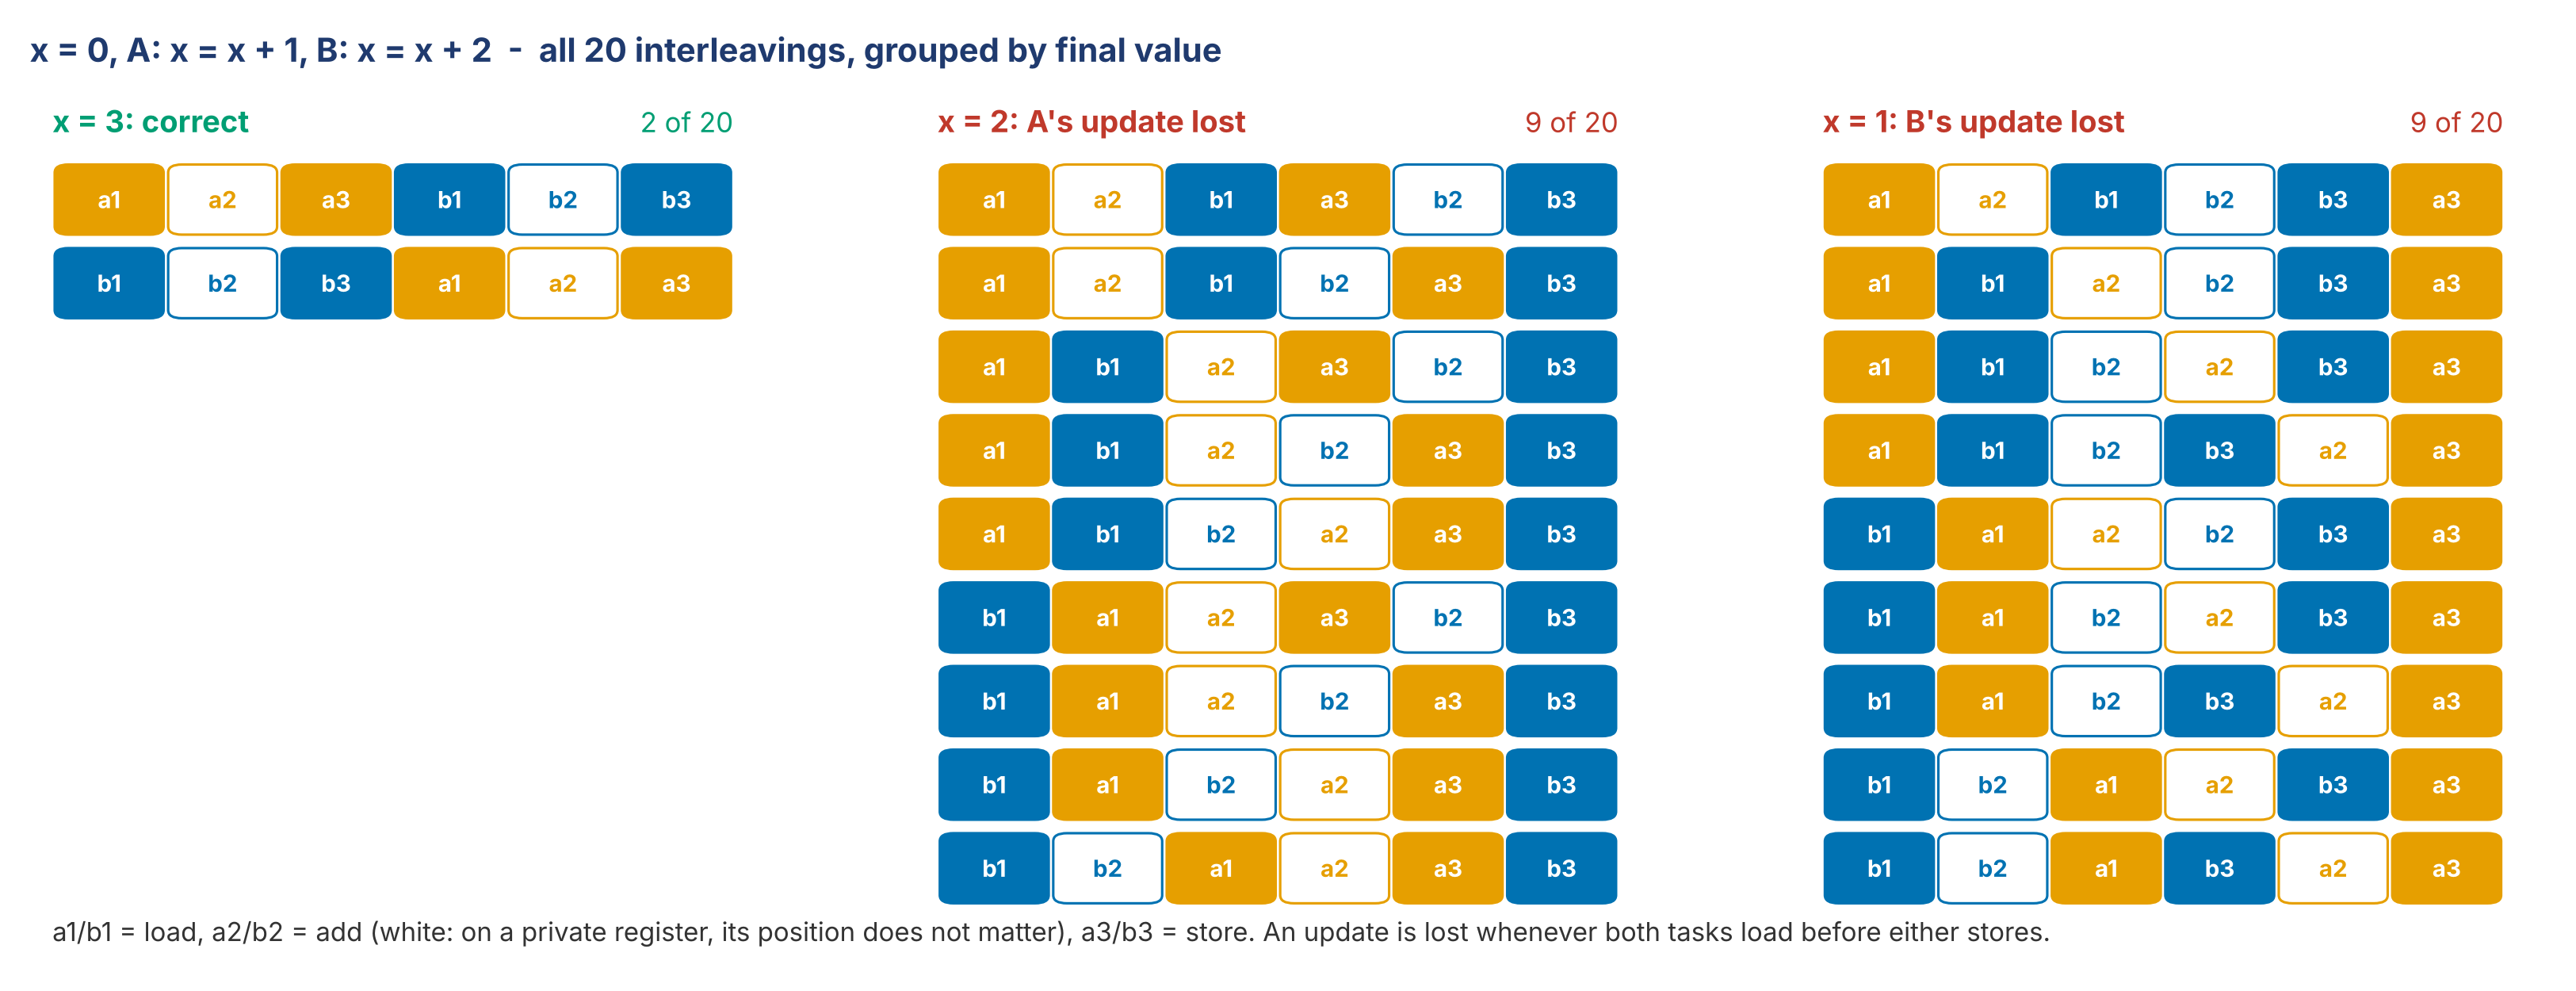
\includegraphics[width=1\textwidth]{contents/images/week-07/interleavings_results.png}
    \caption{All 20 interleavings of \texttt{x = x + 1} (A) and \texttt{x = x + 2} (B), from \texttt{x = 0}. Only the two sequential orders give 3; in the other 18 both tasks load 0 before either stores, and the last store wins. The white cells (the adds) can move without changing anything: only the order of loads and stores matters.}
\end{figure}
With a problem like this you should, potentially, try \textbf{all possible combinations} of the single instructions, to understand everything that can go wrong.

\subsection{Try it on paper: interleavings}
\texttt{x} is shared and starts at 1. Task A runs \texttt{x = x * 2}, task B runs \texttt{x = x + 3}. Each is load, compute, store, on a private register.
\begin{enumerate}
    \item If A runs completely before B, what is the final \texttt{x}? And if B runs completely before A?
    \item List every final value that some interleaving can produce. For each value, write one interleaving with the steps a1 a2 a3 and b1 b2 b3.
    \item Which of these values are correct, if the program does not say which task must go first?
    \item Which values are impossible if a switch can happen only after a store (never between a load and its store)?
\end{enumerate}
\paragraph{Exam.} An exercise on paper like this one in the slides is an indication of a potential \textbf{exam-like exercise}.

\needspace{4\baselineskip}
\textbf{Solution.}
\begin{verbatim}
    order                                final x
    a1 a2 a3 b1 b2 b3   (A then B)       (1 * 2) + 3 = 5
    b1 b2 b3 a1 a2 a3   (B then A)       (1 + 3) * 2 = 8
    a1 b1 b2 b3 a2 a3   (A stores last)  both load 1, A stores 1 * 2 = 2
    a1 b1 a2 a3 b2 b3   (B stores last)  both load 1, B stores 1 + 3 = 4
\end{verbatim}
\begin{enumerate}
    \item A before B gives 5; B before A gives 8.
    \item Four values: 2, 4, 5, 8. If one task stores before the other one loads, the second one sees the first one's result, and you get 5 or 8. If both tasks load before either stores, both start from 1: the task that stores last wins, and you get 2 (A last: $1 \times 2$) or 4 (B last: $1 + 3$).
    \item 5 and 8: each is what one sequential order gives. 2 and 4 are lost updates.
    \item 2 and 4: they need both loads before the first store. If each load-compute-store cannot be cut, only 5 and 8 remain. Making the three steps one critical section is exactly what fixes it.
\end{enumerate}

\subsection{Solution 1: mask interrupts}
Fewer exercises today: the point is how to solve the problem in reality. One solution is very simple, needs no new code and works: \textbf{mask the interrupts} while in a critical section. Think of how the scheduler works: round robin, so the tasks are switched by the tick interrupt; if the tick cannot arrive, the task cannot be stopped. On one CPU a task loses the CPU only in two ways: an \textbf{interrupt} (the tick, then PendSV), or its \textbf{own call} (\texttt{task\_yield}, \texttt{task\_delay}, exit). If the critical section masks interrupts and makes no such call, no other task can run inside it: mask before entering, work, restore at the end, problem solved.

It was already done in week 3: in \texttt{drivers/uart.c}, \texttt{uart\_write} masks interrupts while it copies bytes into the TX ring, because the UART interrupt handler uses the same indices:
\begin{lstlisting}[language=C, showstringspaces=false]
    uint32_t saved = irq_save();     /* old PRIMASK, then PRIMASK = 1: masked   */
    /* ... copy bytes into tx_buf, move tx_head ...                             */
    irq_restore( saved );            /* PRIMASK = saved: unmasked only if it was */
\end{lstlisting}
\texttt{irq\_save} in \texttt{kernel/irq.s} is two instructions and a return: \texttt{mrs r0, primask} reads the old mask into \texttt{r0} (the return value), and \texttt{cpsid i} masks interrupts (PRIMASK $=$ 1). \texttt{irq\_restore} writes the saved value back. Saving the old value, instead of simply unmasking at the end, lets one masked section run inside another: the inner \texttt{irq\_restore} puts back ``masked'', and only the outer one unmasks.

\paragraph{Where is the problem?} (A question to the class.) Forgetting to unmask locks the system for ever, but that is a \textbf{bad programmer}'s problem, true of every lock. The real problem is one even the best programmer cannot solve: in our kernel, a task \textbf{cannot mask} at all.

\subsection{The limits of masking}
Masking works, but it has four limits (privilege, its reason, latency, one CPU):
\begin{itemize}
    \item \textbf{Privileged only}: the masking instruction was used in the boot code (interrupts masked during the bootstrap, then restored), and it is \textbf{privileged}: \texttt{cpsid i} changes PRIMASK only in privileged mode. Our tasks are unprivileged (week 4), and in unprivileged mode the instruction is simply ignored: no fault, no effect.
    \item That is \textbf{on purpose}, and reasonable: a task that could mask interrupts could do a lot of bad things in the operating system, e.g.\ stop the tick and keep the CPU for ever, and the whole protection of week 4 would be gone.
    \item So it is a nice and simple solution only in a \textbf{flat} operating system, which runs everything privileged. That is possible: many operating systems do not exploit kernel and user mode or memory protection. There you can build two simple primitives, \textbf{lock} (disable interrupts) and \textbf{unlock} (enable them again): one instruction each, minimal changes.
    \item \textbf{Latency}: while interrupts are masked, the system \textbf{does not respond to anything}: every interrupt waits, even an urgent one that has nothing to do with the shared data (it is not lost, it is just not served until the unmask). The section must be super small: if it is bigger than a few assembly instructions, be careful.
    \item \textbf{One CPU only}: on a multi-core chip, masking acts only on its own core. If a task on core 0 masks, core 1 still reacts to interrupts, and its task can enter the same section at the same time; and one core cannot mask the interrupts of another, because masking means running the instruction on that core. Still, single-core CPUs are a large set of embedded applications.
\end{itemize}
So masking is a good tool \textbf{inside the kernel}, for a few instructions: the kernel runs privileged, and wants something simple. Tasks need something else.

\subsection{Try it: \texttt{make DEMO=cpsid run}}
Goal: check that a task cannot protect its \texttt{printf} by masking interrupts. This build is \texttt{DEMO=race} with each \texttt{printf} between \texttt{cpsid i} and \texttt{cpsie i} (the macros \texttt{PRINT\_BEGIN} and \texttt{PRINT\_END} in \texttt{src/tasks.h}), executed in user mode.
\begin{lstlisting}[language=bash]
    make DEMO=cpsid run
\end{lstlisting}
What you see, in one run (same notation as before):
\begin{lstlisting}[literate={×}{{$\times$}}1 {←}{{$\leftarrow$}}1 {…}{{\ldots}}1]
    B×100
    B×64 A×100         ← B's line is cut again
    A×100
       … about 390 lines of A …
    B×36               ← the rest of B's line
\end{lstlisting}
\begin{itemize}
    \item The lines still mix: 12 broken lines in this run. There is no fault either: the CPU ran \texttt{cpsid i} in user mode and ignored it.
    \item The tick kept coming, so the quantum ended in the middle of a line, exactly as without the instructions.
\end{itemize}

\subsection{Why a plain flag fails}
The other idea is to work at the \textbf{software level}: a shared word \texttt{busy}, 0 = free, 1 = taken, with \textbf{busy waiting} on it. Each task does:
\begin{lstlisting}[language=C, showstringspaces=false]
    while ( busy == 1 ) { }      /* entry: wait until free */
    busy = 1;                    /* entry: take it          */
    /* ... critical section ... */
    busy = 0;                    /* exit: give it back      */
\end{lstlisting}
It does not work: the \textbf{test} (\texttt{busy == 1}) and the \textbf{update} (\texttt{busy = 1}) are different instructions, and the task can be interrupted between them. One interleaving, with \texttt{busy = 0} at the start:
\begin{enumerate}
    \item A reads \texttt{busy = 0} and leaves its loop. A tick switches to B, before A writes 1.
    \item B reads \texttt{busy = 0}, leaves its loop, writes 1 and enters its critical section. A tick switches to A, inside B's section.
    \item A continues where it stopped: it writes 1 and enters too. Both are inside: \textbf{no mutual exclusion}.
\end{enumerate}

\begin{figure}[H]
\centering
\resizebox{\textwidth}{!}{%
\begin{tikzpicture}[x=1cm, y=0.9cm, font=\scriptsize, >=Stealth,
    lab/.style={anchor=east, font=\scriptsize\bfseries}]
    \node[lab] at (-0.15,2) {task A};
    \node[lab] at (-0.15,1) {task B};
    \node[lab] at (-0.15,0) {\texttt{busy}};
    \foreach \y in {2,1} \draw[gray!35] (0,\y-0.3) rectangle (15.5,\y+0.3);
    % A
    \draw[blue!60!black, fill=blue!20] (0,1.7) rectangle (2.4,2.3); \node at (1.2,2) {read \texttt{busy} $= 0$};
    \draw[blue!60!black, fill=blue!20] (9.6,1.7) rectangle (12,2.3); \node at (10.8,2) {write \texttt{busy = 1}};
    \draw[red!70!black, fill=red!15] (12,1.7) rectangle (15.5,2.3); \node at (13.75,2) {\textbf{critical section}};
    % B
    \draw[orange!80!black, fill=orange!25] (3,0.7) rectangle (5.4,1.3); \node at (4.2,1) {read \texttt{busy} $= 0$};
    \draw[orange!80!black, fill=orange!25] (5.4,0.7) rectangle (7.8,1.3); \node at (6.6,1) {write \texttt{busy = 1}};
    \draw[red!70!black, fill=red!15] (7.8,0.7) rectangle (9,1.3); \node at (8.4,1) {\textbf{c.s.}};
    \draw[red!70!black, fill=red!8, dashed] (12,0.7) rectangle (15.5,1.3); \node at (13.75,1) {B: still inside its section};
    % switches
    \foreach \x in {2.7,9.3} { \fill[black] (\x-0.15,-0.5) rectangle (\x+0.15,2.5); }
    \node[above] at (2.7,2.5) {tick: switch};
    \node[above] at (9.3,2.5) {tick: switch};
    % busy values
    \node at (1.2,0) {0}; \node at (4.2,0) {0}; \node at (8.4,0) {1}; \node at (12.5,0) {1 (written again by A)};
    \draw[->] (0,-0.75) -- (15.7,-0.75) node[right] {time};
    \node[text=red!70!black, font=\scriptsize\bfseries] at (13.75,-0.35) {both tasks inside: no mutual exclusion};
\end{tikzpicture}}
\caption{Why a plain flag fails. The test (read \texttt{busy}) and the set (write 1) are two steps: A is switched out between them, B finds the flag still free and enters, and when A resumes it sets the flag and enters too.}
\end{figure}

The entry section is itself a \textbf{read-then-write race}, the same problem it should solve: the lost update again, on the flag instead of the counter. A software solution could work only if the test and the assignment were \textbf{one atomic step}.

\subsection{Hardware help: atomic read-modify-write}
This is where hardware comes to rescue us all: \textbf{without hardware support there is no solution}. As always, operating systems are software designed \textbf{together with computer architects}: the two communities design the hardware and the software together, and many CPUs have specific instructions that do two operations at the same time, in an atomic way.
\begin{itemize}
    \item The fix needs the read and the write of the flag to be one atomic step: an \textbf{atomic read-modify-write}. Software alone cannot build it on one CPU without masking interrupts: the hardware must provide it.
    \item The classic one is \textbf{test-and-set}: in one step, read the old value of a word and write 1 into it (test a condition, and set a value, atomically).
\end{itemize}
\begin{lstlisting}[language=C, showstringspaces=false, basicstyle=\ttfamily\footnotesize]
/* what the hardware does, in ONE step that nothing can cut */
uint32_t test_and_set( uint32_t *p ) { uint32_t old = *p; *p = 1; return old; }

void lock( uint32_t *l )   { while ( test_and_set( l ) == 1 ) { } }   /* 1: taken, try again */
void unlock( uint32_t *l ) { *l = 0; }
\end{lstlisting}
\begin{itemize}
    \item If \texttt{test\_and\_set} returns 0, the word was free and you set it: you \textbf{hold the lock}. If it returns 1, someone else holds it, and your write of 1 changed nothing (it was already 1).
    \item Two tasks can no longer both see 0: the first one's read and write happen together, so the second one reads the 1 that the first one wrote.
    \item Many CPUs have such an instruction: the Intel x86 has read-modify-write and test-and-set instructions (e.g.\ \texttt{xchg}, which swaps a register and a word). The Cortex-M3 has none: as always, ARM does it in a different way, which makes things a bit more complex.
\end{itemize}

\subsection{The Cortex-M3 way: \texttt{ldrex} and \texttt{strex}}
ARM is a \textbf{RISC} processor: few, simple instructions, none of which can do a complex job such as a read and a write together. So the Cortex-M3 splits the atomic step into \textbf{two} instructions that work together, a load and a store whose names end in \texttt{ex} (\emph{exclusive}):
\begin{lstlisting}[basicstyle=\ttfamily\footnotesize]
    ldrex r1, [r0]        @ r1 = *r0, and start watching: "exclusive access begins"
    strex r2, r1, [r0]    @ if nothing happened since ldrex: *r0 = r1, r2 = 0
                          @ else: store nothing, r2 = 1 (failed)
\end{lstlisting}
\begin{itemize}
    \item \textbf{\texttt{ldrex}} (load exclusive) is, from a functional point of view, a normal \texttt{ldr}: it loads the word pointed by \texttt{r0} into \texttt{r1}, and also says ``I want to update this word''. But as soon as it runs, it starts a \textbf{watching mechanism}: a small hardware component watches what happens to the memory location just loaded. It tells the processor: ``now I hold this value, and if somebody tries to change it, I need to know''.
    \item \textbf{\texttt{strex}} (store exclusive) is, functionally, a normal store of \texttt{r1} at the address in \texttt{r0}, and it is where you find out whether somebody changed the word. It stores only if nothing could have touched the word since the \texttt{ldrex}; otherwise it \textbf{fails} and stores nothing. Its first register tells which: \texttt{r2 = 0} stored, \texttt{r2 = 1} failed.
    \item If \texttt{strex} fails, you simply start again from the \texttt{ldrex}, and read the new value.
    \item Between the two you can compute anything: test the old value, add 1, \dots\ So the pair gives test-and-set, an atomic increment, and more: copy the shared value into a register with \texttt{ldrex}, do whatever you want with it, then try to write the result back with \texttt{strex}.
\end{itemize}
The pair is \textbf{not} ``uninterruptible'': an interrupt can still come between the two. It is ``either nothing came in between, or the store does not happen and you know it''.

\subsection{The exclusive monitor}
Who decides that ``nothing happened''? A small piece of hardware, the \textbf{exclusive monitor}, with two states:
\begin{itemize}
    \item \textbf{Open} (nothing watched) and \textbf{Exclusive} (one address watched): \texttt{ldrex} sets Exclusive; \texttt{strex} stores only in Exclusive, and \textbf{always} sets it back to Open. So a \texttt{strex} in Open stores nothing and returns 1.
    \item \textbf{Any exception entry or return} sets the monitor to Open (tick, UART interrupt, PendSV, system call), even without a switch.
    \item On one CPU another task runs only after an exception (the tick and PendSV, or a system call): so the rule ``every exception clears the monitor'' is enough. A \texttt{strex} preempted after its \texttt{ldrex} \textbf{fails}, and the task retries with the new value: A never overwrites B's work.
\end{itemize}

\begin{figure}[H]
\centering
\resizebox{\textwidth}{!}{%
\begin{tikzpicture}[font=\scriptsize, >=Stealth,
    st/.style={draw, rounded corners=3pt, minimum width=2.6cm, minimum height=0.9cm, align=center},
    lab/.style={anchor=east, font=\scriptsize\bfseries}]
    % state machine
    \node[st] (open) at (0,0) {\textbf{\small Open}\\nothing watched};
    \node[st, fill=blue!55, text=white, draw=blue!70!black] (exc) at (7,0) {\textbf{\small Exclusive}\\one address watched};
    \draw[->, thick] (open.north) to[bend left=25] node[above] {\texttt{ldrex}} (exc.north);
    \draw[->, thick] (exc.west) -- node[above] {\texttt{strex} $\to$ 0: stored} (open.east);
    \draw[->, thick, blue!70!black] (exc.south) to[bend left=25] node[below, font=\scriptsize\bfseries] {any exception entry or return} (open.south);
    \draw[->, thick] (open.west) to[out=150, in=210, looseness=5] (open.west);
    \node[align=right, anchor=east] at (-2.3,0) {\texttt{strex} $\to$ 1:\\nothing stored};
    % example timeline
    \node[font=\scriptsize\bfseries, anchor=west] at (-2.2,-2.1) {example: A is preempted between its \texttt{ldrex} and its \texttt{strex}};
    \begin{scope}[yshift=-2.6cm, font=\tiny]
    \node[lab] at (-1.6,0) {task A};
    \node[lab] at (-1.6,-0.7) {task B};
    \node[lab] at (-1.6,-1.4) {kernel};
    \node[lab] at (-1.6,-2.1) {monitor};
    \foreach \y in {0,-0.7,-1.4} \draw[gray!35] (-1.5,\y-0.25) rectangle (11.4,\y+0.25);
    \fill[blue!55] (-1.5,-0.25) rectangle (1.2,0.25); \node[text=white] at (-0.15,0) {\texttt{ldrex}: lock $= 0$};
    \fill[blue!55] (7.6,-0.25) rectangle (11.4,0.25); \node[text=white] at (9.5,0) {\texttt{strex} $\to$ 1; retry: lock $= 1$};
    \fill[blue!70!black] (2.2,-0.95) rectangle (6.6,-0.45); \node[text=white] at (4.4,-0.7) {\texttt{ldrex}, \texttt{strex} $\to$ 0: B has the lock};
    \fill[black] (1.3,-1.65) rectangle (2.1,-1.15); \node[text=white] at (1.7,-1.4) {tick};
    \fill[black] (6.7,-1.65) rectangle (7.5,-1.15); \node[text=white] at (7.1,-1.4) {switch};
    \draw (-1.5,-2.35) rectangle (1.2,-1.85); \node at (-0.15,-2.1) {Exclusive};
    \draw (1.2,-2.35) rectangle (2.2,-1.85); \node at (1.7,-2.1) {Open};
    \draw (2.2,-2.35) rectangle (6.6,-1.85); \node at (4.4,-2.1) {Exclusive};
    \draw (6.6,-2.35) rectangle (11.4,-1.85); \node at (9,-2.1) {Open: A's \texttt{strex} fails, nothing stored};
    \end{scope}
\end{tikzpicture}}
\caption{The exclusive monitor. Top: \texttt{ldrex} opens an exclusive access, \texttt{strex} closes it (storing only if it was still Exclusive), and any exception closes it too. Bottom: A reads the free lock, the tick clears the monitor, B takes the lock, and when A runs again its \texttt{strex} finds the monitor Open and fails.}
\end{figure}

The monitor does not compare values: A's \texttt{strex} fails because the exceptions set the monitor to Open, which happens whenever another task could have run. This is how a \textbf{test-and-set} is implemented on an ARM CPU.

\subsection{A lock with \texttt{ldrex} and \texttt{strex}}
First at a high level, then (Unit 2) in assembly. A primitive that waits until it has permission to enter a critical section is an \textbf{infinite loop}: load the lock variable and check that it is 0 (1 means the critical section is locked: continue, another round); if it is 0, try to change it to 1 with \texttt{strex}, then check whether the write succeeded. If it did (the first argument is 0), break the loop: you may enter the critical section. If not, spin again. In pseudo-code (C cannot write \texttt{ldrex} and \texttt{strex} directly):
\begin{lstlisting}[language=C, showstringspaces=false, basicstyle=\ttfamily\footnotesize]
void lock( uint32_t *l )
{
    for ( ;; )
    {
        if ( ldrex( l ) != 0 ) continue;   /* taken: look again             */
        if ( strex( l, 1 ) == 0 ) break;   /* stored 1, nobody came between */
    }                                      /* strex failed: start again     */
    dmb();                                 /* barrier: next subsection      */
}

void unlock( uint32_t *l ) { dmb(); *l = 0; }    /* a plain store is enough */
\end{lstlisting}
\begin{itemize}
    \item A task that reads 0 with \texttt{ldrex} and stores 1 with \texttt{strex} without failing \textbf{holds the lock}.
    \item \texttt{unlock} needs no exclusive store: only the holder writes the word at that moment. The other task's \texttt{strex} writes only after its \texttt{ldrex} read 0, which cannot happen while the lock is 1.
\end{itemize}

\subsection{Memory barrier: \texttt{dmb}}
Before going down to assembly, one more danger: all these operations are \textbf{memory accesses}, and modern CPUs \textbf{reorder} instructions and memory accesses to optimise execution: to be fast, a CPU and its memory system may let memory accesses \textbf{complete in a different order} than in the program, very often on bigger cores than ours. It is done in hardware: even if the assembly has three instructions in a row, the hardware may run them in a different order, because it is smart enough to see that the order can change without changing the output of the program (the compiler may reorder them too). On the few instructions that implement synchronization this is very dangerous.
\begin{itemize}
    \item For a lock it would be fatal: a write of the critical section could become visible \textbf{after} the unlock store, when another task already holds the lock.
    \item \textbf{\texttt{dmb}} (data memory barrier), an instruction of the ARM set already used before: if the CPU still has pending memory operations, it completes all of them first, and only then moves on. Every memory access before it completes before any memory access after it: a \textbf{synchronization point} in the pipeline.
    \item \textbf{Rule}: \texttt{dmb} \textbf{after taking} the lock (the section's accesses cannot move before it) and \texttt{dmb} \textbf{before releasing} it (they cannot move after it).
    \item The Cortex-M3 is a very simple CPU and reorders very little: the barrier costs almost nothing and rarely changes anything. But move the same code to a more complex core, such as a Cortex-A9 or A53\footnote{The A9 executes instructions out of order; the A53 is in order, but both follow the weakly ordered ARM memory model, where memory accesses can become visible in a different order: on both, barriers are required.}, and accesses really are reordered: with the barrier, the lock stays correct on every ARM core.
\end{itemize}

\subsection{The spinlock}
With these few instructions (\texttt{ldrex}, \texttt{strex} and \texttt{dmb}) a full synchronization primitive takes about \textbf{10 assembly instructions}: the \textbf{spinlock}. Most students studied semaphores and mutexes in previous OS courses: the spinlock is their \textbf{little brother}. It stops you if you cannot enter the critical section, but while you are stopped you do \textbf{busy waiting}; its big brothers are smarter, and put you in a waiting state, so that you do not consume CPU. The name says it: while the lock is taken, the task \textbf{spins} in its loop and tries again and again, consuming CPU.
\begin{itemize}
    \item It works for \textbf{unprivileged} tasks: \texttt{ldrex}, \texttt{strex} and \texttt{dmb} need no privilege, only memory both tasks can write.
    \item On \textbf{two cores} spinning makes sense: the holder runs on the other core and frees the lock soon.
    \item On \textbf{one CPU} it is waste: while B spins, A (the holder) cannot run, so the lock cannot become free. B burns the rest of its quantum (up to 5 ticks $=$ 50\,ms) for nothing.
    \item Better: \textbf{spin-then-yield}. If the lock is taken, call \texttt{task\_yield} (week 5): the holder runs, frees the lock, and you try again at your next turn.
    \item Unit 2 (after the break) builds both, fixes the two demos, and shows the waste in the scheduler trace.
\end{itemize}

\subsection{The semaphore}
The other mechanisms are only seen quickly: the scratch-OS does not implement them, but FreeRTOS has them and we will use them. A spinlock makes the waiting task use the CPU; a \textbf{semaphore} makes it \textbf{sleep}: it is an integer counter, plus a list of tasks BLOCKED on it, with two atomic operations. In the professor's words, a semaphore combines \textbf{three things}:
\begin{enumerate}
    \item a \textbf{shared variable}: an integer counter shared by all the tasks that use the semaphore, so the operating system must allow \textbf{shared memory};
    \item two \textbf{primitives} that test the value and change it \textbf{atomically}: where the lock of a spinlock is only 0 or 1, a semaphore checks whether its variable is different from 0 and then decrements it by one, still a test followed by an update;
    \item the ability to take a task that cannot go on and \textbf{park it in a waiting state}, so that it does not use the CPU, and, when the semaphore is free again, to take a waiting task and put it back in the \textbf{ready queue}: this basically requires modifying the \textbf{scheduler}.
\end{enumerate}
\begin{lstlisting}[basicstyle=\ttfamily\footnotesize]
    wait( S ):     if ( S.count > 0 ) S.count = S.count - 1;
                   else   block the caller: RUNNING -> BLOCKED, put it on S.list
    signal( S ):   if ( S.list is not empty ) move one task: BLOCKED -> READY
                   else   S.count = S.count + 1;
\end{lstlisting}
\begin{itemize}
    \item The two operations are called \textbf{wait} and \textbf{signal}. In some books they are \textbf{P} and \textbf{V}, the names given by Dijkstra, who invented the semaphore, in his paper (Dutch for ``try'' and ``raise''); some systems say down/up, and \textbf{FreeRTOS} says \textbf{take} and \textbf{give}. They always work in the same way.
    \item \texttt{count} is the number of ``permits'' still free. A task that finds none does \textbf{not} spin: it is BLOCKED, and the CPU goes to others. You know the BLOCKED state from week 5: a task in a delay is BLOCKED in the same way.
    \item \texttt{signal} with a waiting task hands the permit straight to it: the count stays the same, because the permit goes from one task to the other without passing through the counter.
    \item The kernel makes \texttt{wait} and \texttt{signal} atomic: in our kernel a system call already runs to completion. The test-and-set part could use exactly the code of the spinlock.
\end{itemize}
The third ingredient needs many more structures in the scheduler and in the operating system: this is why the course skips the implementation of the semaphore in the scratch-OS.

\subsection{Three uses, by initial value}
\begin{center}
\small
\begin{tabular}{P{0.11} P{0.2} P{0.28} P{0.33}}
    \hline
    \textbf{initial count} & \textbf{name} & \textbf{meaning} & \textbf{example} \\
    \hline
    $N > 1$ & counting & $N$ identical resources are free & 3 DMA buffers shared by 5 tasks \\
    1 & binary (mutual exclusion) & one task at a time in the section & \texttt{wait} = entry section, \texttt{signal} = exit section \\
    0 & signalling & ``B waits until A says go'' & B \texttt{wait}s for data; A \texttt{signal}s when it has produced it \\
    \hline
\end{tabular}
\end{center}
\begin{itemize}
    \item The operations are always the same two: only the \textbf{initial count} changes the meaning.
    \item In signalling, the task that waits and the one that signals are different; a task can even signal from an \textbf{interrupt handler}, because \texttt{signal} never blocks.
    \item A signal that comes before the wait is \textbf{not lost}: the count remembers it.
\end{itemize}

\paragraph{One trace each.} The count and the list after each operation:
\begin{center}
\footnotesize
\begin{tabular}{P{0.3} c c P{0.45}}
    \hline
    \textbf{operation} & \textbf{count} & \textbf{list} & \textbf{effect} \\
    \hline
    \multicolumn{4}{l}{\cellcolor{gray!15}\textbf{counting}, count $= 2$} \\
    A \texttt{wait} & 1 & -- & A takes a permit \\
    B \texttt{wait} & 0 & -- & B takes the last one \\
    C \texttt{wait} & 0 & C & C is BLOCKED \\
    A \texttt{signal} & 0 & -- & C becomes READY, it has A's permit \\
    \multicolumn{4}{l}{\cellcolor{gray!15}\textbf{binary}, count $= 1$} \\
    A \texttt{wait} & 0 & -- & A enters the critical section \\
    B \texttt{wait} & 0 & B & B is BLOCKED at the entry \\
    A \texttt{signal} & 0 & -- & A leaves, B becomes READY and enters \\
    B \texttt{signal} & 1 & -- & B leaves, the section is free \\
    \multicolumn{4}{l}{\cellcolor{gray!15}\textbf{signalling}, count $= 0$} \\
    B \texttt{wait} & 0 & B & B blocks: no ``go'' yet \\
    A \texttt{signal} & 0 & -- & ``go'': B becomes READY \\
    (other order) A \texttt{signal} & 1 & -- & the ``go'' is remembered \\
    (other order) B \texttt{wait} & 0 & -- & B continues at once \\
    \hline
\end{tabular}
\end{center}
Look at \texttt{A signal} in the counting and binary traces: the count stays 0, because the permit goes straight to the waiting task. The count goes back up only when a \texttt{signal} finds nobody waiting.

\subsection{The mutex}
The \textbf{mutex} (from \emph{mutual exclusion}) is really the \textbf{big brother} of the spinlock: logically, a single variable that can be only 0 or 1, and 0 means you may enter your critical section. It differs from a spinlock in two ways:
\begin{itemize}
    \item when it is locked, the waiting task does \textbf{not busy-wait}: it is put in a waiting state (BLOCKED), like with a semaphore;
    \item it has an \textbf{owner}: the task that locked it is the \textbf{only one} allowed to unlock it.
\end{itemize}
\begin{itemize}
    \item \texttt{lock( m )}: if free, the caller becomes the owner; if taken, the caller waits (usually BLOCKED).
    \item \texttt{unlock( m )}: allowed only to the owner; the next waiting task becomes the owner. An unlock by another task is an error the kernel can report: the unlock must fail.
\end{itemize}
Semaphores do not have this idea. A \textbf{binary semaphore} (one that takes only the values 0 and 1) is logically a mutex, but with a semaphore one task can wait and \textbf{another} task signal: one task is blocked, and a different one releases it. With a mutex, the task that locks it becomes its owner, and only it can unlock. At the low level the assembly instructions for the test-and-set are the same; the operating system needs more structures: at every successful lock it must record which task locked, and at every unlock it must check which task tries, and make the unlock fail if it is not the same one.
\begin{center}
\begin{tabular}{P{0.25} P{0.33} P{0.33}}
    \hline
    & \textbf{binary semaphore} & \textbf{mutex} \\
    \hline
    has an owner & no & yes \\
    who may release it & any task, or an interrupt handler & only the task that holds it \\
    typical use & mutual exclusion or signalling & mutual exclusion only \\
    release by the wrong task & allowed: a hidden bug & detected as an error \\
    \hline
\end{tabular}
\end{center}
A binary semaphore and a mutex look alike, but the owner makes the difference: with a semaphore, a task that calls \texttt{signal} by mistake opens the door for everybody, and nobody notices; a mutex detects it. The rule of thumb: use a \textbf{mutex to protect data}, and a \textbf{semaphore to count or to signal}.

\subsection{The family of primitives}
To wrap up, a general operating system has four basic families of synchronization primitives (there are many more, but these are found almost everywhere):
\begin{center}
\small
\begin{tabular}{P{0.15} P{0.23} c P{0.23} P{0.2}}
    \hline
    \textbf{primitive} & \textbf{how a task waits} & \textbf{owner} & \textbf{what for} & \textbf{runs in} \\
    \hline
    interrupt masking & nobody can wait: no switch at all & -- & a few instructions in the kernel, one CPU & privileged code only \\
    spinlock & spins on the CPU (or spins, then yields) & no & short sections; best with several cores & any code, with \texttt{ldrex}/\texttt{strex} \\
    semaphore & blocks: BLOCKED until a \texttt{signal} & no & counting, mutual exclusion, signalling & the kernel (system calls) \\
    mutex & usually blocks & yes & mutual exclusion & the kernel (system calls) \\
    \hline
\end{tabular}
\end{center}
\begin{itemize}
    \item All of them give an entry and an exit section; they differ in \textbf{how the waiting task spends its time}.
    \item Spinlock, semaphore and mutex work on the \textbf{same low-level mechanism} (the atomic test-and-set), plus, for the last two, more machinery connected to the scheduler: they need a kernel that can block a task. The spinlock needs only the atomic instructions: that is why Unit 2 starts with it.
\end{itemize}

\subsection{Try it on paper: final exercises}
Once you understand how the primitives work, you can do simple exercises: take some instructions, surround them with synchronization primitives, and see how the program reacts.
\begin{enumerate}
    \item \textbf{Two increments each.} \texttt{x} is shared and starts at 0. Tasks A and B each run \texttt{x = x + 1} twice (each time: load, add, store). What is the largest possible final \texttt{x}? What is the smallest? Give an interleaving for the smallest, and explain why 1 is impossible.
    \item \textbf{Initial values.} For each case, choose the initial count of the semaphore and the use (counting, binary, signalling):
    \begin{enumerate}
        \item 4 tasks share a pool of 2 identical radio channels;
        \item two tasks update the same linked list;
        \item task B must start its work only after the UART interrupt handler has received a byte;
        \item what happens if the semaphore of (b) starts at 0 by mistake?
    \end{enumerate}
    \item \textbf{A trace.} A semaphore starts at 1. In order: A \texttt{wait}, B \texttt{wait}, C \texttt{wait}, A \texttt{signal}, B \texttt{signal}. After each step, write the count, the list, and who is inside.
\end{enumerate}

\needspace{4\baselineskip}
\textbf{Solution.}
\begin{enumerate}
    \item The largest is \textbf{4}: no overlap, every increment sees the previous one. The smallest is \textbf{2}. One interleaving that gives 2:
    \begin{itemize}
        \item A loads 0 (and keeps it in its register);
        \item B does one whole increment: load 0, add, store, so $x = 1$;
        \item A adds and stores 1 (its register held 0): $x = 1$;
        \item B loads 1 for its second increment;
        \item A does its second increment completely: load 1, add, store, so $x = 2$;
        \item B adds and stores 2 (its register held 1): $x = 2$.
    \end{itemize}
    Why 1 is impossible: every store writes at least 1, because every load reads at least 0. Now look at the \textbf{last} store of the run. It belongs to some task's \textbf{second} increment (a task's second store comes after its first one). That second increment loaded \textbf{after} the same task's own first store, which wrote at least 1, and nobody ever writes a smaller value than 1. So it loaded at least 1, and it stores at least 2.
    \item (a) 2, counting. (b) 1, binary (a mutex fits too). (c) 0, signalling: the handler \texttt{signal}s, B \texttt{wait}s. (d) The first task that calls \texttt{wait} blocks, and so does every other: nobody ever enters, nobody ever signals, the tasks wait for ever (\textbf{progress} is broken).
    \item
    \begin{tabular}[t]{l c l l}
        \hline
        \textbf{step} & \textbf{count} & \textbf{list} & \textbf{inside} \\
        \hline
        A \texttt{wait} & 0 & -- & A \\
        B \texttt{wait} & 0 & B & A \\
        C \texttt{wait} & 0 & B, C & A \\
        A \texttt{signal} & 0 & C & B (READY with A's permit) \\
        B \texttt{signal} & 0 & -- & C (READY with B's permit) \\
        \hline
    \end{tabular}

    At each \texttt{signal} a task is waiting, so the permit goes straight to it, and the count stays 0 until the end.
\end{enumerate}

\paragraph{From the class discussion: exercise 1.} Why 1 is impossible must be \textbf{explained} as in the solution, not stated: an answer such as ``because B overwrites'' is not understandable at the exam. A side remark: a real compiler would probably turn two \texttt{x = x + 1} in a row into \textbf{one} load, two adds and \textbf{one} store; the exercise assumes, as stated, a load-add-store per increment.

\paragraph{Protecting the increments.} A semaphore or a mutex both work: with a semaphore initialised to \textbf{1}, each task calls \texttt{wait} before \texttt{x = x + 1} and \texttt{signal} at the end of each operation.

\begin{figure}[H]
    \centering
    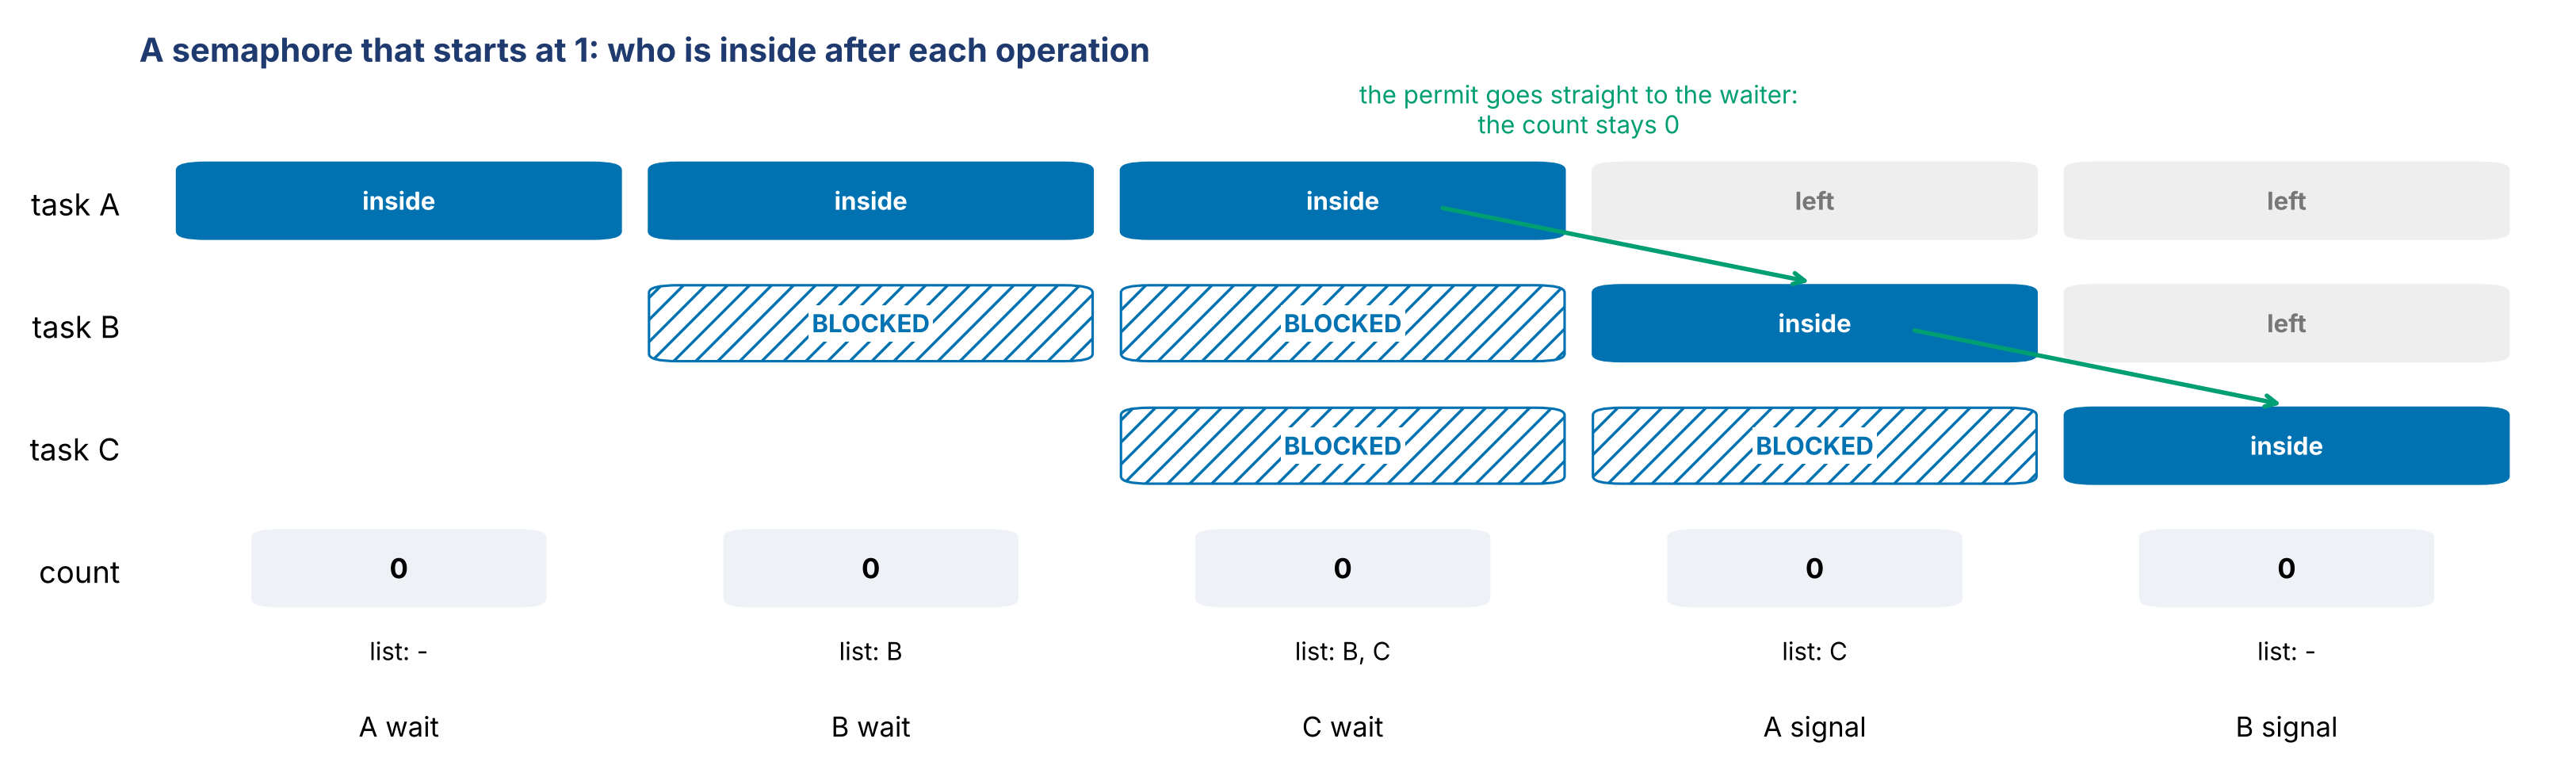
\includegraphics[width=1\textwidth]{contents/images/week-07/semaphore_trace.png}
    \caption{Exercise 3 as a picture. A enters; B and C block in the semaphore's list; each \texttt{signal} hands the permit straight to a waiting task, so the count stays 0 from the first \texttt{wait} to the end.}
\end{figure}

\paragraph{From the class discussion: exercise 3, who enters?} Three tasks call \texttt{wait} on a semaphore initialised to 1: which one enters? Not necessarily A. A task can call \texttt{wait} and be interrupted at once: the one that enters is the \textbf{first that manages to run} \texttt{wait}, and the \textbf{scheduler} decides which task runs. The table assumes that A gets inside and B and C wait; if B were the running task at that moment, B would be first. Likewise, when A signals, the critical section is free and B \emph{or} C may enter: the table says B, but there is no rule on the order. With a scheduler that takes the waiting tasks first come, first served, and the order B, C, you get B; another scheduler may follow any other rule.

\paragraph{Never rely on the order.} You \textbf{never} build synchronization on the order in which the tasks happen to run: it must work \textbf{regardless of the order}, assuming that the way the scheduler works is \textbf{unknown}. An application that works only because the tasks are queued in a certain way breaks the day an update of the operating system changes the scheduler (for performance or security reasons): if it assumes that after this \texttt{signal} B runs next, and the new scheduler runs C first, it fails. Build only on what the primitives guarantee: \texttt{wait} lets you enter if the semaphore is greater than 0 and stops you if it is 0; once blocked, you have no idea when you will run again, only that when the semaphore is positive again you get a \emph{chance} to run, and the scheduler decides, in a way you do not know.

\paragraph{The restroom.} One restroom in a bar, several people waiting. When the door opens somebody can enter, but the owner of the bar decides who goes first; you may complain that you were first in line, but he is the owner. He promises only two things: if the restroom is free and you want to enter, you may go (\textbf{progress}); and you will not wait there for ever, at some point you will get your chance (\textbf{bounded waiting}). These guarantees come from building the primitives properly; the application must rely on nothing else.

\section{Unit 1: summary}
\begin{itemize}
    \item Two tasks that share something (a variable, a buffer, a device such as the UART) can interfere: \texttt{DEMO=race} mixes lines because one \texttt{printf} line needs two atomic \texttt{sys\_write} calls; \texttt{DEMO=counter} loses updates because \texttt{x = x + 1} is load, add, store.
    \item A \textbf{race condition} is a result that depends on the interleaving; the \textbf{critical section} is the smallest piece of code that must not be cut by another task's section on the same resource. A test that passes proves nothing: reason on every interleaving.
    \item A correct entry/exit protocol guarantees \textbf{mutual exclusion}, \textbf{progress} and \textbf{bounded waiting}, for any speed.
    \item \textbf{Masking interrupts} works only in privileged code, for very short sections, on one CPU: good inside the kernel. A plain flag fails, because test and set are two steps.
    \item The hardware gives an \textbf{atomic read-modify-write}: test-and-set on x86; \texttt{ldrex}/\texttt{strex} and the exclusive monitor on the Cortex-M3 (any exception clears the monitor, so a preempted \texttt{strex} fails and retries). \texttt{dmb} after taking and before releasing a lock.
    \item \textbf{Spinlock}: busy waiting, about 10 instructions, unprivileged. \textbf{Semaphore}: counter plus a list of BLOCKED tasks, \texttt{wait}/\texttt{signal} (P/V, take/give); counting, binary or signalling by initial value. \textbf{Mutex}: a blocking lock with an owner.
    \item Synchronization must never rely on the order in which the scheduler runs the tasks: which waiting task enters is the scheduler's choice, and only the guarantees of the primitives (mutual exclusion, progress, bounded waiting) may be assumed.
\end{itemize}

\section{Unit 2 - A spinlock in the scratch-OS}
After a 10-minute break, the rest of the lecture is a real implementation of a spinlock: forget the complex high-level mechanisms for now. In the next two weeks, with FreeRTOS, there will be a lot of exercises with semaphores and mutexes, and plenty of time for the high-level, application side; today the time goes to the \textbf{low level}, to see how much complexity there is.

\subsection{From the theory to the scratch-OS}
In this unit, file paths are relative to \texttt{scratch-os/week-07/solution/}; you work in \texttt{scratch-os/week-07/base/}, where the lock functions are still empty. Unit 1 showed the races of \texttt{make DEMO=race} and \texttt{make DEMO=counter}, and the spinlock on paper. This unit writes that spinlock and fixes both races.
\begin{itemize}
    \item There was no new implementation last week (theory only), so the starting point is the kernel of \textbf{week 5}: \texttt{week-07/base/} is that kernel (round robin, \texttt{task\_yield}, the trace) with the same two-phase program in tasks A and B: a shared counter, then 3000 lines of letters each.
    \item The tasks already take a lock around every counter update and every \texttt{printf}. The lock functions exist, but each one is a single \texttt{bx lr}: they do nothing yet.
    \item You write only one new file, \texttt{lib/spinlock.s}, in two steps: first a plain busy-waiting lock, then a spin-then-yield lock. It is in \textbf{assembly}, because the spinlock needs the two exclusive instructions: assembly is the only way to build this synchronization primitive (even when called from C, specific assembly instructions must run).
    \item After each step you run the program, check the result, and read the scheduler trace to see what the lock costs.
    \item The finished code is in \texttt{week-07/solution/}, with every line commented.
\end{itemize}
Before the lock, two prepared pieces need explaining: where the shared data lives, and how the tasks call the lock.

\subsection{Tasks cannot share memory}
The first change is the \textbf{memory layout}. Since week 4 the MPU keeps each task in its own 4\,KB partition: region 0 is FLASH, read-only for everybody; region 1 is the running task's partition, moved at every switch by \texttt{mpu\_set\_task\_region} (\texttt{kernel/mpu.c}); any other access is a MemManage fault. So A and B had no variable in common. The base adds a \textbf{1\,KB shared region} at \texttt{0x20003000}, right after the three partitions (A, B, idle), opened to both tasks by a third MPU region, \textbf{region 2}, readable and writable and \textbf{always active}. Only variables placed there are shared: stacks and line buffers stay private.
A synchronization primitive is, first of all, a \textbf{variable}: the shared variables of the locks go in this region.

\begin{figure}[H]
\centering
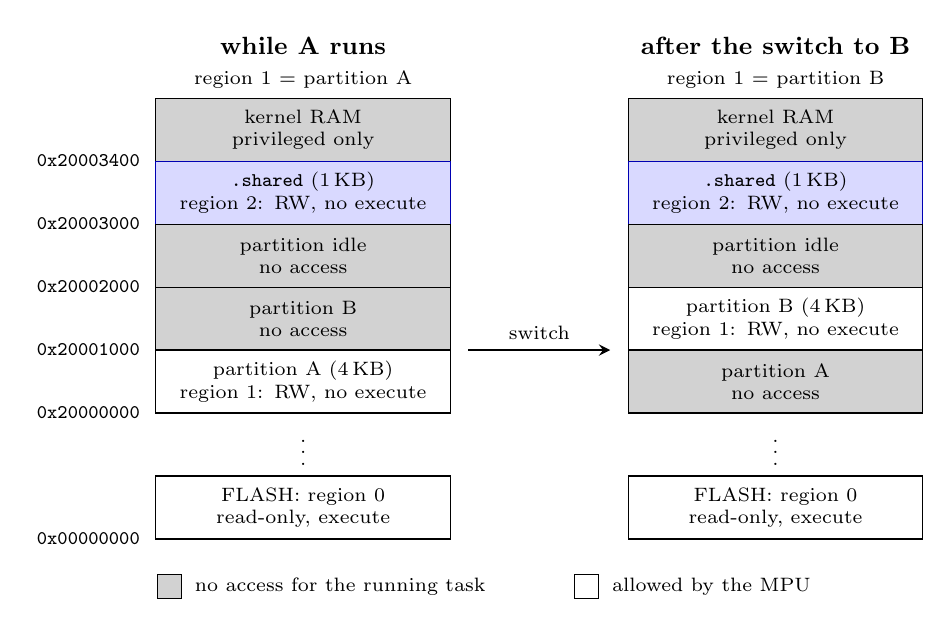
\begin{tikzpicture}[font=\scriptsize,
    mem/.style={draw, text width=3.6cm, minimum height=0.8cm, align=center, inner sep=2pt},
    ok/.style={mem, fill=white},
    no/.style={mem, fill=gray!35},
    sh/.style={mem, fill=blue!15, draw=blue!70!black}]
    % left: while A runs
    \node[font=\small\bfseries, align=center] at (0,4.85) {while A runs\\{\scriptsize\normalfont region 1 = partition A}};
    \node[no] at (0,4.0) {kernel RAM\\privileged only};
    \node[sh] at (0,3.2) {\texttt{.shared} (1\,KB)\\region 2: RW, no execute};
    \node[no] at (0,2.4) {partition idle\\no access};
    \node[no] at (0,1.6) {partition B\\no access};
    \node[ok] at (0,0.8) {partition A (4\,KB)\\region 1: RW, no execute};
    \node at (0,0) {$\vdots$};
    \node[ok] at (0,-0.8) {FLASH: region 0\\read-only, execute};
    \foreach \y/\a in {3.6/0x20003400, 2.8/0x20003000, 2.0/0x20002000, 1.2/0x20001000, 0.4/0x20000000, -1.2/0x00000000}
        \node[left, font=\scriptsize\ttfamily] at (-1.95,\y) {\a};
    % right: after the switch to B
    \node[font=\small\bfseries, align=center] at (6,4.85) {after the switch to B\\{\scriptsize\normalfont region 1 = partition B}};
    \node[no] at (6,4.0) {kernel RAM\\privileged only};
    \node[sh] at (6,3.2) {\texttt{.shared} (1\,KB)\\region 2: RW, no execute};
    \node[no] at (6,2.4) {partition idle\\no access};
    \node[ok] at (6,1.6) {partition B (4\,KB)\\region 1: RW, no execute};
    \node[no] at (6,0.8) {partition A\\no access};
    \node at (6,0) {$\vdots$};
    \node[ok] at (6,-0.8) {FLASH: region 0\\read-only, execute};
    \draw[->, >=stealth, thick] (2.1,1.2) -- node[above] {switch} (3.9,1.2);
    % legend
    \node[draw, fill=gray!35, minimum size=0.3cm] at (-1.7,-1.8) {};
    \node[right] at (-1.5,-1.8) {no access for the running task};
    \node[draw, fill=white, minimum size=0.3cm] at (3.6,-1.8) {};
    \node[right] at (3.8,-1.8) {allowed by the MPU};
\end{tikzpicture}
\caption{The shared region in the memory map (not to scale). Region 1 moves at every switch; regions 0 and 2 stay the same, so the 1\,KB block \texttt{.shared} at \texttt{0x20003000} is open to whichever task runs. In the build, \texttt{nm build/scratch-os.axf} shows \texttt{shared\_counter} at \texttt{0x20003000}, \texttt{counter\_lock} at \texttt{0x20003014} and \texttt{uart\_lock} at \texttt{0x20003018}.}
\end{figure}

\paragraph{The shared variables.} The RAM now has four blocks before the kernel's data: the partitions of A, B and the idle task (4\,KB each), and the 1\,KB shared region. The shared variables are defined in \texttt{src/shared.c}:
\begin{itemize}
    \item \texttt{shared\_counter}, the counter both tasks add to;
    \item \texttt{shared\_counter\_done\_a} and \texttt{shared\_counter\_done\_b}: ``I have finished the counter phase'', one word per task, so that each task writes only its own word;
    \item \texttt{shared\_all\_done\_a} and \texttt{shared\_all\_done\_b}: ``I have finished everything'', used to decide which task is the last one and prints the trace;
    \item \texttt{counter\_lock} and \texttt{uart\_lock}, the two locks.
\end{itemize}

\paragraph{Two changes in practice.} (1) The \textbf{linker script}: a new memory section, where the shared variables are placed. (2) The \textbf{MPU}: program it, at start-up, to protect that section and make it readable and writable, i.e.\ write specific values into its control registers (week 4).

\paragraph{Why 1\,KB, and not less?} (A question to the class.) Alignment, and the MPU rules: a region has a power-of-two size, starts at a multiple of its size, and is at least 32 bytes. Without the MPU, the shared block could have exactly the size you want: from now on, every change to the OS must respect the decisions of the previous weeks.

\subsection{Inspect: the shared region}
The section \texttt{.shared} in \texttt{scripts/mps2\_m3.ld}, and region 2 in \texttt{mpu\_init} in \texttt{kernel/mpu.c}:
\begin{lstlisting}[basicstyle=\ttfamily\scriptsize]
.shared ALIGN(1024) (NOLOAD) :
{
    _shared_start = .;                  /* first byte of the block - the MPU region 2 starts here */
    *(.shared .shared.*)                /* every variable marked SHARED in the C files */
    . = _shared_start + 1024;           /* always exactly 1 KB, the size of the MPU region */
    _shared_end = .;                    /* end of the block (exclusive) */
} > RAM
\end{lstlisting}
\begin{lstlisting}[language=C, showstringspaces=false, basicstyle=\ttfamily\scriptsize]
MPU->RBAR = (uint32_t) _shared_start | MPU_RBAR_VALID | 2;    /* start from the linker script */
MPU->RASR = MPU_RASR_XN | MPU_RASR_AP( MPU_AP_FULL_RW )
          | MPU_RASR_S | MPU_RASR_C
          | MPU_RASR_SIZE( 9 ) | MPU_RASR_ENABLE;             /* 1 KB: 0x13060013 */
\end{lstlisting}
\begin{itemize}
    \item \texttt{ALIGN(1024)} starts the block at a multiple of 1\,KB: after the three 4\,KB partitions, that is \texttt{0x20003000}.
    \item \texttt{\_shared\_start} and \texttt{\_shared\_end} are \textbf{linker symbols}: the C code can use their addresses.
    \item \texttt{*(.shared .shared.*)} collects every input section called \texttt{.shared} from all the object files: every variable marked \texttt{SHARED}.
    \item \texttt{. = \_shared\_start + 1024} makes the block exactly 1\,KB, however few variables it holds, so that it matches the MPU region.
    \item \texttt{(NOLOAD)}: see the first question below.
    \item \textbf{Region 2}, registers known from week 4: \texttt{RBAR} gets the start address, the VALID bit and the region number 2: $\texttt{0x20003000} \,|\, \texttt{0x10} \,|\, 2 = \texttt{0x20003012}$. \texttt{RASR} gets execute-never (\texttt{XN}), full read-write access for privileged and unprivileged code (\texttt{AP = 3}), the shareable and cacheable bits, the size field 9 (a region of $2^{9+1} = 1024$ bytes) and the enable bit: together \texttt{0x13060013}.
\end{itemize}
A variable goes there with the \texttt{SHARED} marker of \texttt{src/shared.h}:
\begin{lstlisting}[language=C, showstringspaces=false, basicstyle=\ttfamily\footnotesize]
#define SHARED __attribute__(( section( ".shared" ) ))
\end{lstlisting}
This asks the compiler to put the variable in a section called \texttt{.shared} instead of the usual \texttt{.bss} or \texttt{.data}, and the linker script does the rest; for example, \texttt{src/shared.c} has \texttt{volatile uint32\_t shared\_counter SHARED;}. The slide asks three questions: (1) Why can a shared variable not have a start value, such as \texttt{= 5}? (2) Why does region 2 never change when the kernel switches tasks? (3) \texttt{sys\_write} accepts a buffer only inside the caller's partition or FLASH: why does \texttt{printf( "counter=\%u ...", shared\_counter )} still work?

\needspace{4\baselineskip}
\textbf{Solution.}
\begin{enumerate}
    \item \textbf{\texttt{NOLOAD}}: the linker reserves the RAM but stores nothing for it in FLASH: there is no image of the shared section in FLASH, which saves time and space, and the section is initialised at run time. So \texttt{Reset\_Handler} copies no start values there; RAM is zero at start, so every shared variable starts at 0, and a \texttt{= 5} would be silently lost. For the locks this is exactly what you want: \textbf{0 means free}, so every spinlock starts not taken.
    \item Region 2 is \textbf{fixed}: \texttt{mpu\_init} sets it once at boot, with full read-write access for unprivileged code. A switch rewrites only region 1 (\texttt{mpu\_set\_task\_region}), so the shared block is open to whichever task runs. \texttt{ALIGN(1024)} and the 1\,KB size are MPU rules from week 4: a region is a power of two in size, and starts at a multiple of its size. \texttt{XN} forbids running code from the shared data.
    \item \texttt{printf} \textbf{copies}: it formats into its own 64-byte buffer, on the task's stack, inside the task's partition, and only that buffer's address reaches \texttt{sys\_write}; \texttt{shared\_counter} itself is passed \textbf{by value}, as a number in a register. So the kernel's pointer check in \texttt{sys\_write\_impl} in \texttt{kernel/syscall.c} was not changed: the shared region never reaches \texttt{sys\_write}.
\end{enumerate}

\subsection{Inspect: the lock calls}
The code uses many \texttt{\#define}s and macros (to inspect slowly at home), so that \textbf{one application program} changes behaviour depending on the demo being built. \texttt{LOCK} and \texttt{UNLOCK} in \texttt{src/tasks.h}, and the body of the counter loop in \texttt{task\_a} in \texttt{src/task\_a.c} (\texttt{task\_b} in \texttt{src/task\_b.c} is the same):
\begin{lstlisting}[language=C, showstringspaces=false, basicstyle=\ttfamily\scriptsize]
#if defined( DEMO_RACE ) || defined( DEMO_COUNTER ) || defined( DEMO_CPSID )
#define LOCK( l )   do { } while ( 0 )      /* no lock: the race shows */
#define UNLOCK( l ) do { } while ( 0 )      /* no lock: the race shows */
#elif defined( DEMO_SPIN )
#define LOCK( l )   spin_lock_busy( l )     /* take it, busy waiting */
#define UNLOCK( l ) spin_unlock( l )        /* give it back */
#else
#define LOCK( l )   spin_lock( l )          /* take it, yield while taken */
#define UNLOCK( l ) spin_unlock( l )        /* give it back */
#endif

    LOCK( &counter_lock );                          /* only one task at a time below */
    shared_counter = plus_one( shared_counter );    /* load, add 1, store */
    UNLOCK( &counter_lock );                        /* the other task may update now */
\end{lstlisting}
\begin{itemize}
    \item In the race demos, \texttt{LOCK} is a \texttt{do \{ \} while ( 0 )}: a loop whose condition is false, so it exits at once: it does nothing, and so does \texttt{UNLOCK}. It is the usual way to write a macro that does nothing but still needs a \texttt{;} after it, like a function call. All the demos run so far (\texttt{DEMO=race}, \texttt{DEMO=counter}, \texttt{DEMO=cpsid}) used this ``implementation'', which is why the printed letters depended on the order, and the final counter changed at every run.
    \item Two more implementations: a spinlock with \textbf{busy waiting} (\texttt{spin\_lock\_busy}), and a smarter one with less busy waiting (\texttt{spin\_lock}). The application always calls \texttt{LOCK} and \texttt{UNLOCK}, in capitals: the Makefile decides which functions they become.
    \item \texttt{spinlock\_t} in \texttt{lib/spinlock.h} is a \texttt{volatile uint32\_t}: 0 = free, 1 = taken. \texttt{volatile} tells the compiler that the word can change behind its back (the other task writes it), so it must really read and write memory at every use. \texttt{counter\_lock} and \texttt{uart\_lock} are in the shared region.
    \item Questions: (1) Why does \texttt{LOCK} get the \textbf{address} of the lock? (2) In the base, all three functions are just \texttt{bx lr}: what does \texttt{make run} print?
\end{itemize}

\needspace{4\baselineskip}
\textbf{Solution.}
\begin{center}
\begin{tabular}{P{0.36} P{0.3} P{0.26}}
    \hline
    \textbf{build} & \texttt{LOCK( l )} \textbf{becomes} & \texttt{UNLOCK( l )} \textbf{becomes} \\
    \hline
    \texttt{DEMO=race}, \texttt{DEMO=counter}, \texttt{DEMO=cpsid} & nothing & nothing \\
    \texttt{DEMO=spin} & \texttt{spin\_lock\_busy( l )} & \texttt{spin\_unlock( l )} \\
    default (\texttt{make run}) & \texttt{spin\_lock( l )} & \texttt{spin\_unlock( l )} \\
    \hline
\end{tabular}
\end{center}
\begin{enumerate}
    \item The address: the function must read and change the word in the shared region itself, not a copy of its value: a copy would be a private register, and changing it would tell the other task nothing. By the AAPCS, the calling rules of ARM, the address arrives in \texttt{r0}, the first argument.
    \item The base: \texttt{make run} calls the empty functions, so nothing is protected. It prints what Unit 1's race demos printed: a total below 2\,000\,000 and mixed lines. Even the \texttt{counter=} line can come out cut inside a line of letters, because one task can still be printing its lines while the other one prints its total.
\end{enumerate}
Each \texttt{printf} is wrapped in the same way with \texttt{uart\_lock}. There are \textbf{two} locks, one per shared thing: a task that prints holds \texttt{uart\_lock}, and does not stop the other one from counting with \texttt{counter\_lock}. One lock for everything would also be correct, but the two tasks would wait for each other more than needed.

\subsection{Taking the lock in assembly}
We now write \texttt{spin\_lock\_busy}, line by line. It is called from C as \texttt{void spin\_lock\_busy( spinlock\_t *l )}, so by the calling convention its parameter, the \textbf{address} of the lock, is in \texttt{r0}. Taking the lock means: read it; if it is 0, write 1, and be sure that nothing came in between. Unit 1's exclusive pair does exactly this: \texttt{ldrex}, compare with 0 (taken: read again), \texttt{mov r1, \#1}, \texttt{strex}, check \texttt{r2} (failed: start again), \texttt{dmb}, return. The listing and the instruction-by-instruction explanation are in the ``Try it'' below.

\paragraph{Question: one monitor per lock?} The monitor is associated with a memory \textbf{address}: tasks on the same lock share it, tasks on different locks use different watches. Their number is limited, and we assume there are enough\footnote{The Cortex-M3 has a single local monitor, which watches the address of the last \texttt{ldrex}: a new \texttt{ldrex} simply replaces the previous one. This is enough for a spinlock, whose \texttt{ldrex} is always followed by its own \texttt{strex}, with no other exclusive access in between.}.

\paragraph{Question: why the barrier after the \texttt{strex}?} The window to protect from other tasks is between \texttt{ldrex} and \texttt{strex}; the barrier is about something else, much lower level. The pipeline starts work before it is needed, and memory accesses already in flight could complete in another order. \texttt{dmb} makes every pending memory transaction complete before going on. On our Cortex-M3 the code would probably work without it; on a \textbf{complex} or \textbf{multi-core} CPU it is required.

\subsection{Giving the lock back, and the two barriers}
The opposite operation, \texttt{spin\_unlock}, is simple: it only writes the lock back from 1 to 0. Must we worry whether that write is atomic? No: it is a plain store, and when you unlock you know that every other task is locked out, so nobody can do anything to the lock; once 0 is written in memory, the spinlock is released. It is three instructions and a return: \texttt{dmb}, \texttt{mov r1, \#0}, \texttt{str r1, [r0]}, \texttt{bx lr} (the ARM can only store registers, so 0 goes into a register first; the address of the lock is again the argument, in \texttt{r0}).
\begin{itemize}
    \item A \textbf{plain store} is enough: only the holder may give the lock back, and while you hold it the other task never writes the word (its \texttt{strex} only writes when it read 0).
    \item \texttt{dmb} \textbf{after the take}: the reads and writes of \texttt{shared\_counter} must not start before the lock is yours.
    \item \texttt{dmb} \textbf{before the give-back}: your write to \texttt{shared\_counter} must be finished before the other task can see the lock free. (The example from class: if the hardware swapped a pending write of 1 and the unlock's write of 0, the lock would end up 1.)
    \item For the C compiler, the call to a function in another file is already a point it cannot move memory accesses across.
\end{itemize}
\paragraph{\texttt{dmb} as a checkpoint.} Think of it as ``before the next step, finish whatever is pending on memory'' (like: finish all the exercises of the first seven weeks before starting FreeRTOS). Complex CPUs are fast precisely because they reorder, keep stores in internal buffers and \textbf{commit} them later; every barrier throws those optimisations away and goes back to \textbf{sequential execution}. So barriers go only where order matters, and synchronization is one of those points.

\subsection{Try it: write \texttt{spin\_lock\_busy} and \texttt{spin\_unlock}}
Open \texttt{lib/spinlock.s} and copy the assembly code there. Under the label \texttt{spin\_lock\_busy:}, replace the two stub lines (the marker comment and \texttt{bx lr}) with these lines, keeping the \texttt{.size} line after them; \texttt{spin\_lock\_busy\_try} is a second label at the same address, for the loop:
\begin{lstlisting}[basicstyle=\ttfamily\scriptsize]
spin_lock_busy:
spin_lock_busy_try:
    ldrex r1, [r0]               /* value = *lock, and start watching *lock */
    cmp r1, #0                   /* is value == 0 (free)? */
    bne spin_lock_busy_try       /* if (value != 0) goto try: taken, ask again */
    mov r1, #1                   /* r1 = 1: the value that means "taken" */
    strex r2, r1, [r0]           /* r2 = strex(lock, 1): 0 = written, 1 = not */
    cmp r2, #0                   /* did the write happen? */
    bne spin_lock_busy_try       /* if (r2 != 0) goto try: something came in between */
    dmb                          /* dmb(): the protected accesses start only now */
    bx lr                        /* return: the lock is ours */
\end{lstlisting}
Then do the same under the label \texttt{spin\_unlock:}:
\begin{lstlisting}[basicstyle=\ttfamily\scriptsize]
spin_unlock:
    dmb                          /* dmb(): every earlier access is done first */
    mov r1, #0                   /* r1 = 0: the value that means "free" */
    str r1, [r0]                 /* *lock = 0: the lock is free */
    bx lr                        /* return */
\end{lstlisting}
\paragraph{The whole function, with its directives.} In \texttt{lib/spinlock.s} of the base each function is a label followed by a marker comment and \texttt{bx lr}. Here is \texttt{spin\_lock\_busy} with the directives around it:
\begin{lstlisting}[basicstyle=\ttfamily\scriptsize]
    .global spin_lock_busy      /* visible to C files */
    .type spin_lock_busy, %function /* it is code */
    .thumb_func                 /* it is Thumb code (bit 0 set in its address) */
spin_lock_busy:
spin_lock_busy_try:
    ...                         /* the nine instructions above */
    .size spin_lock_busy, . - spin_lock_busy /* record its size in bytes */
\end{lstlisting}
The directives are the same as for the system-call stubs of week 4: \texttt{.global} makes the name visible to the C files, \texttt{.type} and \texttt{.thumb\_func} say that it is a Thumb function (so its address has bit 0 set when C calls it), and \texttt{.size} records its length for the debugger and the map file. \texttt{spin\_lock\_busy\_try} is a second label \textbf{at the same address} as \texttt{spin\_lock\_busy}: the function could branch to its own name, but a separate label says what the branch means, ``try again''.

\paragraph{Instruction by instruction}, with the lock word at \texttt{[r0]}\footnote{In class the meaning of \texttt{r2} was once said the other way round (``if \texttt{r2} is equal to 0, the store failed''): the convention is the one of the slides and of the code, \texttt{r2 = 0} written, \texttt{r2 = 1} failed, so \texttt{bne} retries when \texttt{r2} is not 0.}:

This is the low-level core of every lock: a semaphore or a mutex contains the same code, and does something smarter than busy waiting. It is also one of the parts of an OS that \textbf{cannot be generic}: another CPU has other instructions, and this code must be rewritten for every port.

\subsection{Try it: run \texttt{DEMO=spin}}
Goal: check that the lock fixes both races. \texttt{DEMO=spin} runs both phases, with \texttt{LOCK = spin\_lock\_busy}:
\begin{lstlisting}[language=bash]
    cd week-07/base
    make DEMO=spin run
\end{lstlisting}
Quit QEMU with \texttt{Ctrl-C} once \texttt{all tasks finished} appears. Before you look: what total do you expect, and can a line still be mixed? What you see:
{\verbatimscriptsize
\begin{verbatim}
scratch-os: kernel started
scheduler: round robin, quantum 5 ticks
A: hello from task A
B: hello from task B
AAAAAAAAAAAAAAAAAAAAAAAAAAAAAAAAAAAAAAAA...    (3000 lines of 100 A's in this run)
task A exited (tick 214)
counter=2000000 expected=2000000 (B last)
BBBBBBBBBBBBBBBBBBBBBBBBBBBBBBBBBBBBBBBB...    (3000 lines of 100 B's)
TRACE BEGIN
...
TRACE END 252
...
task B exited (tick 253)
all tasks finished
\end{verbatim}}
\begin{itemize}
    \item \texttt{counter=2000000}: no update is lost, on every run. Every one of the 6000 lines is whole: 100 letters, all the same. You never see a broken line, simply because every \texttt{printf} is between a lock and an unlock.
    \item The problems of \texttt{printf} are all still there: the task \textbf{can} still be interrupted in the middle of a line, but then the other task does nothing useful (it waits on the lock), and when the first one runs again it goes on printing the same line.
    \item It is a spinlock, a \textbf{stupid} mechanism: it does not put the waiting task in a waiting state; it simply does no useful work while it runs.
    \item In this run A counted, then printed its lines while B was still counting: the two phases of the two tasks overlap, and the order changes from run to run. That is fine: the locks make each update and each line atomic, not the whole program.
    \item But look at the last tick: about 250. The finish time also changes a lot from run to run: in the professor's runs, from about 210 to about 280. The next subsections explain why.
\end{itemize}

\subsection{Why a preempted task's \texttt{strex} fails}
The exclusive monitor of Unit 1, now in the real code. A reads 0 with \texttt{ldrex}, and a tick switches to B before A's \texttt{strex}.
\begin{itemize}
    \item The exception clears the monitor: on the Cortex-M3 \textbf{every} exception entry and return does, even a tick that switches nothing.
    \item B takes the lock: its own \texttt{ldrex} reads 0, its \texttt{strex} succeeds. Back in A, the \texttt{strex} finds the monitor clear: it writes nothing and returns 1, so A retries, reads 1 and waits.
    \item So \texttt{PendSV\_Handler} in \texttt{kernel/pendsv.s} needs no \texttt{clrex}, the instruction that clears the monitor by hand. Some kernels must run it at every switch, but on the Cortex-M3 the exception itself already did it. (The optional gdb session at the end of this unit lets you watch exactly this case in a real run.)
\end{itemize}

\subsection{Try it: the \texttt{DEMO=spin} trace}
Goal: see where the time goes. As in week 5, the last task prints the trace, and \texttt{schedsim} draws it. In \texttt{week-07/base}:
\begin{lstlisting}[language=bash]
    make DEMO=spin run | tee output.txt
    python3 ../../../course-material/tools/schedsim/schedsim.py trace output.txt
\end{lstlisting}
Stop QEMU with \texttt{Ctrl-C} once you see \texttt{all tasks finished}, then run \texttt{schedsim}; the trace holds 64 records, enough for the whole run here. Each record \texttt{T <tick> <from> <to>} is one switch, as in week 5: \texttt{T 5 A B}, \texttt{T 10 B A}, \texttt{T 15 A B}, \dots, every 5 ticks. Look at the slots of A and B: is anything different from the round robin of week 5? The first 65 ticks of the chart (\texttt{schedsim} prints the whole run, much wider):
{\verbatimscriptsize
\begin{verbatim}
trace: ticks 5..219 (214 ticks, 37 switches); time 0 = tick 5
time   0    5    10   15   20   25   30   35   40   45   50   55   60   65
       |....|....|....|....|....|....|....|....|....|....|....|....|....|.
A      .....#####.....#####.....#####.....#####.....#####.....#####.....##
B      #####.....#####.....#####.....#####.....#####.....#####.....#####..
CPU    BBBBBAAAAABBBBBAAAAABBBBBAAAAABBBBBAAAAABBBBBAAAAABBBBBAAAAABBBBBAA
\end{verbatim}}
\begin{itemize}
    \item A and B alternate in whole 5-tick slots until one task exits; then the other runs alone until the end.
    \item The chart looks exactly like week 5's round robin: it \textbf{cannot} show which slots did useful work. A task that spins is RUNNING, for the kernel, like a task that counts.
\end{itemize}
Question: during the counter phase, what did A do in the slots that started while B held \texttt{counter\_lock}?

\needspace{4\baselineskip}
\textbf{Solution.}
\begin{itemize}
    \item A \textbf{spun for the whole slot}. B held the lock, and B cannot run while A has the CPU: there is one CPU. So \texttt{ldrex} read 1 again and again, for 5 ticks, until the next tick switched back to B.
    \item This happens almost every time: in the counter loop a task holds \texttt{counter\_lock} during nearly the whole iteration (the call to \texttt{plus\_one}, with its pause, is inside the lock). A tick almost always lands while the running task holds the lock, so the next slot is wasted.
    \item Only when a tick lands in the short gap between \texttt{UNLOCK} and the next \texttt{LOCK} does the other task find the lock free and make progress: that is why the finish time changes so much between runs.
    \item About half of the CPU time of the counter phase is spent spinning: the result is correct, but it costs about 259 ticks on average (about 250 in the run of the notes), against about 112--115 for the base without a lock (and a wrong result).
    \item On one CPU, busy waiting for a lock held by a task that is not running can never succeed before the next switch.
\end{itemize}
In class the traces were not analysed in detail: the only way to work on them is relaxed, at home, looking at the screen column by column, and they are not the important part. What matters is understanding the \textbf{implementation}; if you are not sure how the code turns into an execution, run the demos with the solution and the trace tool, and the code explains perfectly why the tasks are scheduled in that order.

\subsection{Spin-then-yield}
The last improvement. A spinlock is a stupid mechanism, but it can be implemented better: now a task that tries to lock a taken spinlock spends its whole time quantum in an infinite loop, wasting CPU time. Think about why: if you are running and the lock is taken, its owner is \textbf{another} task, which cannot run because you are running, so busy waiting is surely wasted time. On one CPU the holder can only run if the waiter gives the CPU away: as soon as the task sees that the lock is busy, it gives up \textbf{voluntarily} and lets the scheduler run another task, with the call known from week 5, \texttt{task\_yield} (the system call \texttt{svc \#6} in \texttt{lib/syscalls.s}). The task goes to the end of the round-robin queue, and hopefully the task holding the lock gets a chance to run; next time the task is scheduled, if the lock was given back it continues, otherwise it finds the lock taken again and yields again.
\begin{itemize}
    \item \texttt{spin\_lock} does the same as \texttt{spin\_lock\_busy}, with one change: when \texttt{ldrex} reads 1 (taken), it calls \texttt{task\_yield} instead of trying again at once, and tries again when it gets the CPU back.
    \item The waiter then uses a few instructions of its slot instead of all of it, and the holder gets the rest of the time.
    \item If the \texttt{strex} fails (an exception came in between), \texttt{spin\_lock} retries at once, as before: the lock may well be free, and it costs nothing to look.
    \item With two tasks, \texttt{task\_yield} gives the CPU straight back to the holder, which finishes its critical section and gives the lock back.
    \item It still wastes time: the waiter still runs at every one of its turns, only to find the lock taken and yield again, and each such visit costs a system call and two switches. But as soon as it realises it cannot work, it yields to another task.
\end{itemize}

\subsection{Calling a function from assembly}
One important remark: \texttt{spin\_lock} calls a C function, \texttt{task\_yield}, from assembly, with \texttt{bl}, like a C function calls another one; at some point that function returns, so everything must be set up in the proper way. The AAPCS rules already used apply:
\begin{itemize}
    \item \texttt{bl task\_yield} writes \textbf{its} return address into \texttt{lr}. But we are inside \texttt{spin\_lock}, whose \texttt{lr} holds the way back to the task's C code: the call overwrites it, so it must be saved before the call, to be restored after.
    \item A called function may change \texttt{r0}--\texttt{r3} and \texttt{r12}. \texttt{task\_yield} really does: the kernel writes the system call's result (0) into the task's \texttt{r0}. And \texttt{r0} holds the address of the lock: after the call it would be lost.
    \item After the call you still need both: \texttt{r0} is the address of the lock for the next \texttt{ldrex}, and \texttt{lr} is where \texttt{spin\_lock} returns at the end. So save them on the task's stack before the call and restore them after it: \texttt{push \{r0, lr\}} and \texttt{pop \{r0, lr\}}.
    \item \texttt{r1}, \texttt{r2} (and \texttt{r3}) need no saving: they hold nothing before the call that is used after it; \texttt{spin\_lock} sets them again after the call.
\end{itemize}
\paragraph{Question: could one register be saved instead of two?} No, and the slide says why: the C calling convention wants the stack pointer to be a multiple of \textbf{8 bytes} at every call. Each register is 4 bytes, so pushing an \textbf{even} number of them keeps the alignment. Even if \texttt{spin\_lock} had no argument, so that \texttt{r0} needed no saving, you could not push only \texttt{lr}: you would push two registers anyway, wasting 4 bytes, just to keep the alignment.

\subsection{Try it: write \texttt{spin\_lock}}
In \texttt{lib/spinlock.s}, under the label \texttt{spin\_lock:}, replace the two stub lines (the marker comment and \texttt{bx lr}) with these lines, keeping the \texttt{.size} line after them:
\begin{lstlisting}[basicstyle=\ttfamily\scriptsize]
spin_lock:
spin_lock_try:
    ldrex r1, [r0]               /* value = *lock, and start watching *lock */
    cmp r1, #0                   /* is value == 0 (free)? */
    bne spin_lock_wait           /* if (value != 0) goto wait: taken */
    mov r1, #1                   /* r1 = 1: the value that means "taken" */
    strex r2, r1, [r0]           /* r2 = strex(lock, 1): 0 = written, 1 = not */
    cmp r2, #0                   /* did the write happen? */
    bne spin_lock_try            /* if (r2 != 0) goto try: something came in between */
    dmb                          /* dmb(): the protected accesses start only now */
    bx lr                        /* return: the lock is ours */
spin_lock_wait:
    push {r0, lr}                /* save lock and our return address */
    bl task_yield                /* task_yield(); the holder runs meanwhile */
    pop {r0, lr}                 /* restore lock and our return address */
    b spin_lock_try              /* goto try: maybe the lock is free now */
\end{lstlisting}
Compared with \texttt{spin\_lock\_busy}, two things are new:
\begin{itemize}
    \item The \textbf{first} \texttt{bne} goes to \texttt{spin\_lock\_wait} instead of back to the \texttt{ldrex}: a taken lock now means ``give the CPU away''. The \textbf{second} \texttt{bne} (after a failed \texttt{strex}) still goes straight back to \texttt{spin\_lock\_try}.
    \item The four lines of \texttt{spin\_lock\_wait}: \texttt{push \{r0, lr\}} saves the lock address and the return address on the task's stack (PSP, inside the task's partition); \texttt{bl task\_yield} calls the stub, which runs \texttt{svc \#6}, the kernel pends PendSV, and the other task runs; when this task gets the CPU back, \texttt{task\_yield} returns here, and \texttt{pop \{r0, lr\}} restores the two registers; \texttt{b spin\_lock\_try} tries again from the \texttt{ldrex}.
\end{itemize}
One detail: when the lock is taken, \texttt{spin\_lock} runs an \texttt{ldrex} with no \texttt{strex} after it, and the monitor stays Exclusive. That is harmless: the \texttt{svc} in \texttt{task\_yield} is an exception, so it clears the monitor, and in any case the next \texttt{ldrex} starts a new watch.

\begin{figure}[H]
\centering
\begin{tikzpicture}[font=\scriptsize, >=Stealth,
    box/.style={draw, rounded corners=2pt, minimum width=3.8cm, minimum height=0.65cm, align=center, fill=white},
    dec/.style={draw, rounded corners=8pt, minimum width=2.6cm, minimum height=0.65cm, align=center, fill=blue!8, draw=blue!60!black},
    wt/.style={draw, rounded corners=2pt, minimum width=3.6cm, minimum height=0.65cm, align=center, fill=orange!20, draw=orange!80!black}]
    \node[box] (ld) at (0,0) {\texttt{ldrex r1, [r0]}\\read the lock, start watching};
    \node[dec] (free) at (0,-1.3) {\texttt{r1 == 0}? (free)};
    \node[box] (mv) at (0,-2.6) {\texttt{mov r1, \#1}; \texttt{strex r2, r1, [r0]}};
    \node[dec] (ok) at (0,-3.9) {\texttt{r2 == 0}? (written)};
    \node[box, fill=green!12, draw=green!50!black] (dmb) at (0,-5.2) {\texttt{dmb}; \texttt{bx lr}\\the lock is ours};
    \node[wt] (push) at (5.6,-1.3) {\texttt{push \{r0, lr\}}};
    \node[wt] (y) at (5.6,-2.4) {\texttt{bl task\_yield}\\the holder runs meanwhile};
    \node[wt] (pop) at (5.6,-3.5) {\texttt{pop \{r0, lr\}}; \texttt{b spin\_lock\_try}};
    \draw[->] (ld) -- (free);
    \draw[->] (free) -- node[right] {yes} (mv);
    \draw[->] (mv) -- (ok);
    \draw[->] (ok) -- node[right] {yes} (dmb);
    \draw[->] (free) -- node[above] {no: taken} (push);
    \draw[->] (push) -- (y); \draw[->] (y) -- (pop);
    \draw[->] (pop.east) -- ++(0.4,0) |- (ld.east);
    \draw[->] (ok.west) -- ++(-1.0,0) |- (ld.west);
    \node[anchor=east] at (-1.9,-4.15) {no: retry};
    \node[text=gray, align=left, anchor=north] at (5.6,-4.2) {\texttt{spin\_lock\_busy}: the ``no: taken''\\branch goes straight back to \texttt{ldrex}};
\end{tikzpicture}
\caption{\texttt{spin\_lock}. If the lock is taken, the task saves \texttt{r0} and \texttt{lr} (an even number of registers, for the 8-byte alignment), yields, and tries again when it gets the CPU back; if the \texttt{strex} fails, it retries at once. \texttt{spin\_lock\_busy} is the same without the orange branch.}
\end{figure}

\paragraph{Still not perfect.} There is still busy waiting, but it no longer lasts a whole quantum. Imagine a quantum of 10\,ms, and a task that would have to wait only 1\,ms for the lock: it yields immediately, and its next try comes 10\,ms later. That task is penalised quite a lot, but the CPU does no busy waiting: it does something useful for the other tasks.

\subsection{Try it: \texttt{make run} and its trace}
Goal: the default build, with \texttt{LOCK = spin\_lock}. Same steps as for \texttt{DEMO=spin}:
\begin{lstlisting}[language=bash]
    make run | tee output.txt
    python3 ../../../course-material/tools/schedsim/schedsim.py trace output.txt
\end{lstlisting}
Stop QEMU with \texttt{Ctrl-C} once you see \texttt{all tasks finished}, then run \texttt{schedsim}. Check the counter and the lines first; then compare the last tick with \texttt{DEMO=spin}, and look for slots that differ from a plain 5-tick round robin. What you see (first 65 ticks of the chart):
{\verbatimscriptsize
\begin{verbatim}
task B exited (tick 132)
counter=2000000 expected=2000000 (A last)
task A exited (tick 170)
...
trace: ticks 5..170 (165 ticks, 38 switches); time 0 = tick 5
time   0    5    10   15   20   25   30   35   40   45   50   55   60   65
       |....|....|....|....|....|....|....|....|....|....|....|....|....|.
A      ..............................#####..........##########..........##
B      ##############################.....##########..........##########..
CPU    BBBBBBBBBBBBBBBBBBBBBBBBBBBBBBAAAAABBBBBBBBBBAAAAAAAAAABBBBBBBBBBAA
\end{verbatim}}
\begin{itemize}
    \item Correct again: \texttt{counter=2000000}, 6000 whole lines. The last tick changes a little from run to run (here 170, about 171 on average; 169 to 172 in the runs of the notes); the shape does not change.
    \item A \textbf{0-tick slot} is two switch records at the same tick in the raw trace, e.g.\ \texttt{T 5 A B} followed by \texttt{T 5 B A}: at tick 5 A's slice ended, B got the CPU, found the lock taken and yielded at once. It is too short to draw, so the chart has no column for it.
    \item So the holder keeps the CPU for many slots in a row: here B runs from time 0 to time 30, 30 ticks in a row (25 to 45 ticks in the professor's runs).
\end{itemize}

\subsection{Spin vs spin-then-yield}
\begin{figure}[H]
    \centering
    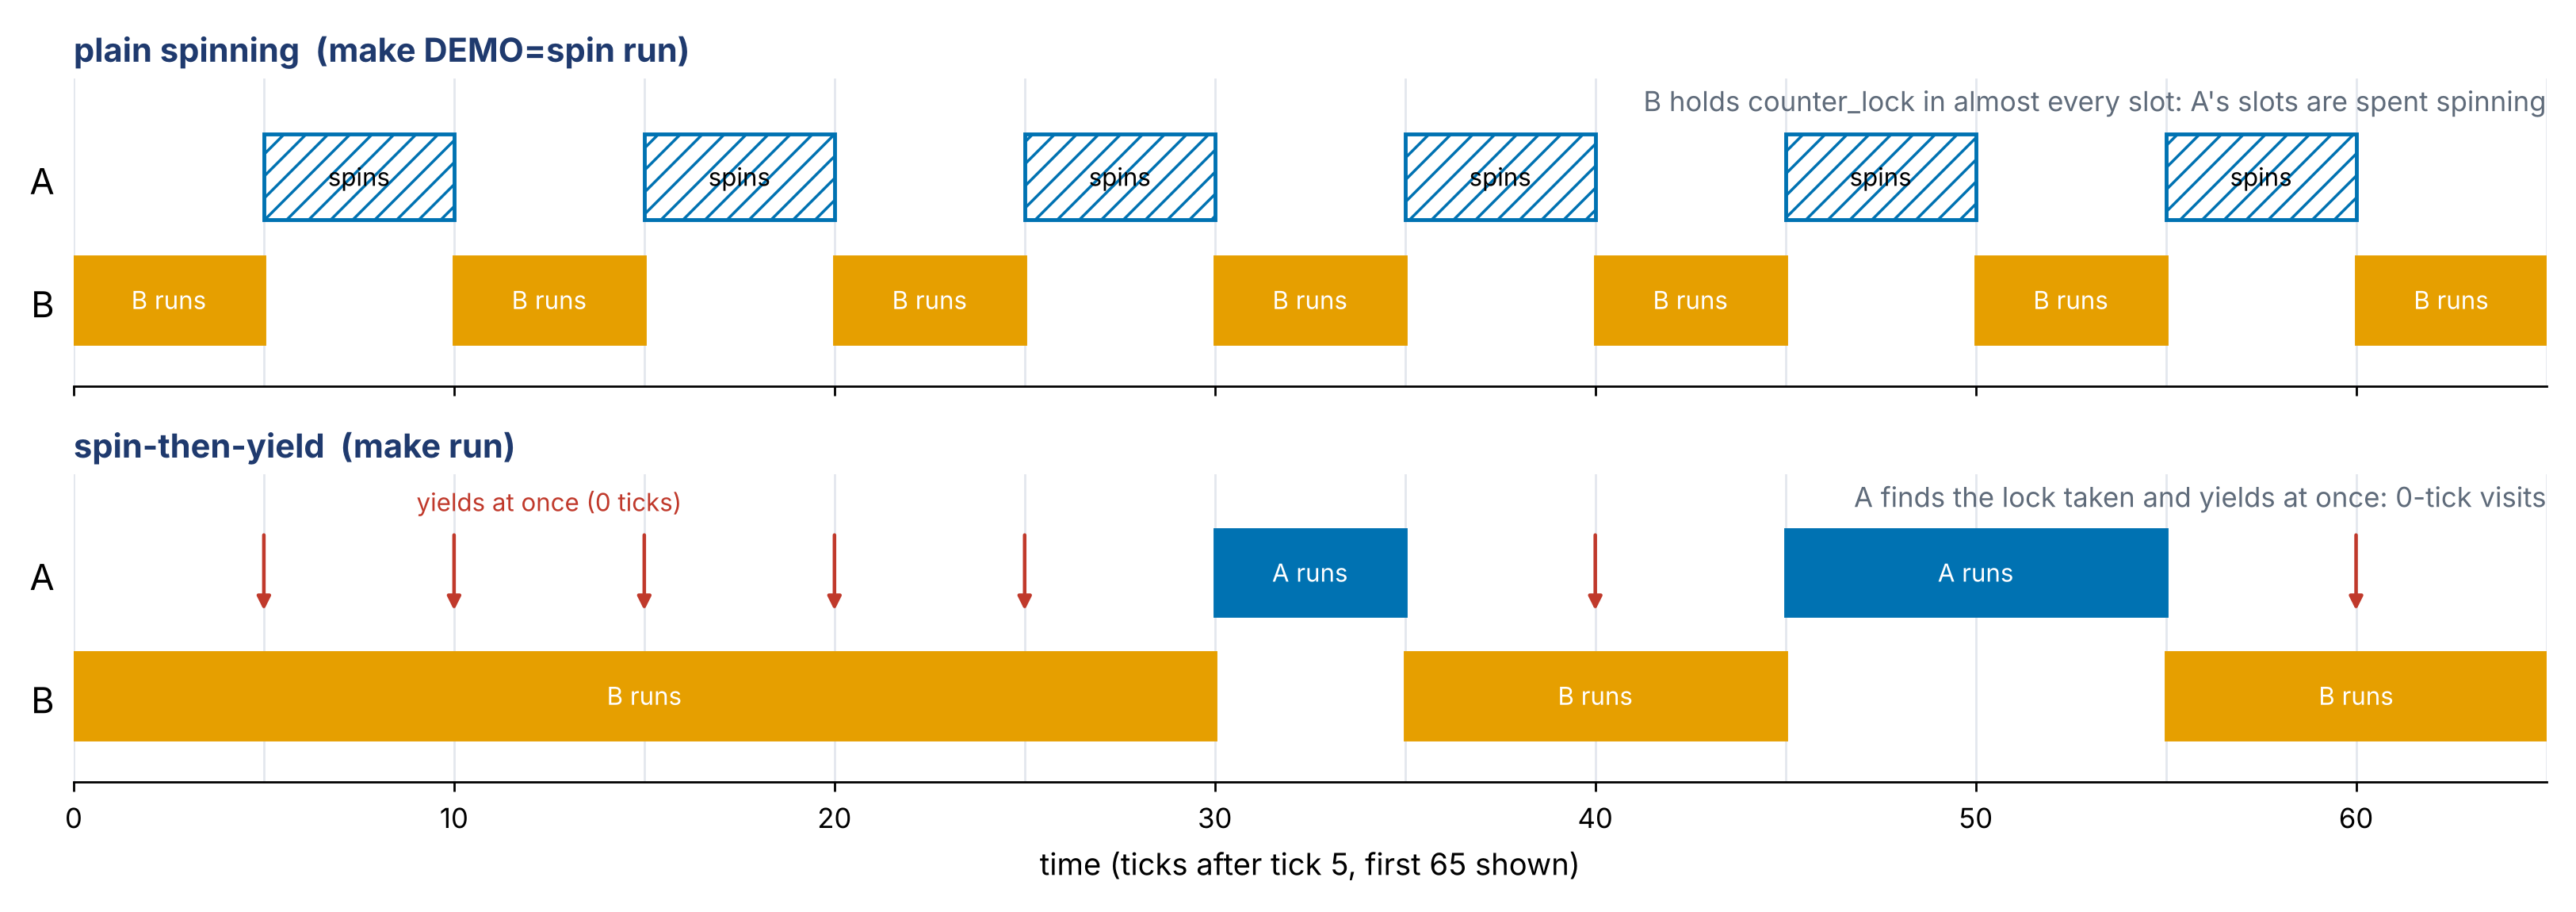
\includegraphics[width=1\textwidth]{contents/images/week-07/spin_vs_yield.png}
    \caption{The first 65 ticks of the two traces (schematic). With plain spinning the chart is a regular round robin, but in the counter phase the waiter's slots are almost all spent spinning, which the trace cannot show. With spin-then-yield the waiter's visits last 0 ticks (red arrows), and the holder keeps the CPU for many slots in a row.}
\end{figure}
One captured run of each build: plain spinning ends at tick 219, spin-then-yield at tick 170. Over 10 runs the average finish is about 259 against about 171; the unprotected run ends at tick 112, but loses updates. Your own runs will differ a little, the busy ones most. Question: spin-then-yield wastes almost no slot, yet it is still slower than no lock at all. Why?

\needspace{4\baselineskip}
\textbf{Solution.}
\begin{center}
\begin{tabular}{P{0.27} P{0.22} P{0.12} P{0.3}}
    \hline
    \textbf{build} & \textbf{lock} & \textbf{result} & \textbf{last tick (average of 10 runs)} \\
    \hline
    base, nothing written & none & wrong & about 112 \\
    \texttt{make DEMO=spin run} & \texttt{spin\_lock\_busy} & correct & about 259 (this run: 219) \\
    \texttt{make run} & \texttt{spin\_lock} & correct & about 171 (this run: 170) \\
    \hline
\end{tabular}
\end{center}
\begin{itemize}
    \item The lock itself costs time: the counter phase makes 2\,000\,000 calls to \texttt{spin\_lock} and as many to \texttt{spin\_unlock}, each with its \texttt{ldrex}, \texttt{strex} and \texttt{dmb}; the lines phase adds 6000 more pairs.
    \item Every visit of the waiter costs too: a system call and two switches, even when its slot lasts 0 ticks. The extra 90 or so ticks of the busy lock are the whole slots spent spinning.
    \item The base without a lock is faster only because it does less work, and its result is wrong: \textbf{a fast wrong answer is no answer}.
    \item Spin-then-yield is also more \textbf{predictable}: about 171 on every run, while the busy version depends on where each tick lands.
\end{itemize}

\subsection{What the spinlock guarantees}
\begin{itemize}
    \item \textbf{Mutual exclusion}: only one task at a time holds the lock. Two tasks can both read 0 with \texttt{ldrex}, but only the first \texttt{strex} after them succeeds. Between the two \texttt{strex} there is at least one exception (the switch from one task to the other), so the second one fails, and its task reads again.
    \item It works in \textbf{unprivileged} code: \texttt{ldrex}, \texttt{strex} and \texttt{dmb} need no privilege, unlike \texttt{cpsid i}, and no system call is needed to take a free lock.
    \item It \textbf{survives preemption}: a task stopped between its \texttt{ldrex} and its \texttt{strex} fails its \texttt{strex} and retries.
    \item \textbf{Progress}: when the lock is free and a task wants it, some task gets it; nobody waits because of a task that is not in the critical section.
    \item Its cost when nobody waits is small: a free lock is taken in about ten instructions.
\end{itemize}

\subsection{What it does not guarantee}
\begin{itemize}
    \item \textbf{No fairness, no bounded waiting}: nothing makes the tasks take the lock in turn. A task may find it taken at each of its turns, as long as the other one is always inside when the tick comes. Bounded waiting, the third requirement of Unit 1, is not met.
    \item \textbf{Waiting still costs}: busy waiting burns whole slots; spin-then-yield burns a system call and two switches per try. Both are fine for short waits, wasteful for long ones.
    \item \textbf{Hold it briefly}: a task that holds the lock for long, or calls \texttt{task\_delay} inside its critical section, makes the other task waste all its turns.
    \item \textbf{No owner check}: \texttt{spin\_unlock} writes 0 whoever calls it. A task that unlocks a lock it does not hold breaks the mutual exclusion silently. (A mutex, with its owner, would catch it.)
    \item \textbf{Not for interrupt handlers}: a handler that spins on a lock held by the task it interrupted would wait for ever, because that task cannot run until the handler ends.
\end{itemize}

\subsection{Why the scratch-OS stops at the spinlock}
Since week 5 the kernel can block tasks: \texttt{task\_delay} makes a task BLOCKED and the tick wakes it. So a blocking lock, where a waiting task sleeps until the lock is free, would be possible.
\begin{itemize}
    \item It would need a list of waiting tasks for each lock, a system call to block on a lock and one to wake the next waiter, and the lock word itself would move into the kernel.
    \item That is a \textbf{choice}, not a missing piece: the spinlock is the simplest primitive of the family, and it is the one that shows the hardware's atomic instructions, which is the point of this unit.
    \item Semaphores and mutexes stay as in Unit 1: you know how they work, and you can tell when a blocking wait is better than spinning.
    \item Unit 3 starts a real kernel, FreeRTOS, on the same board: it has its own blocking primitives, built on the same ideas.
\end{itemize}
This is the \textbf{last operating-system implementation of the semester}. From FreeRTOS on, the kernel is never modified: in the worst case we read how it is implemented (e.g.\ how FreeRTOS implements a semaphore), and most of the code we write is user-level code. FreeRTOS is not complex, but touching a kernel is complicated, and cannot be done in three hours in class.

\paragraph{A memory barrier in the course.} (The professor's joke.) Like a \texttt{dmb}: before moving to FreeRTOS, finish what is pending. Review the first seven weeks, the complex part of the course, and ask about anything still obscure: from now on the pace is more relaxed.

\subsection{Try it on paper: \texttt{ldrex} and \texttt{strex}}
\texttt{L} is a lock in the shared region, \texttt{L = 0}. Both tasks call \texttt{spin\_lock\_busy( \&L )}, so \texttt{r0 = \&L} in both; quantum 5 ticks. The events, in order:
\begin{enumerate}
    \item A: \texttt{ldrex r1, [r0]}
    \item SysTick: A's slice ends, switch to B
    \item B: \texttt{ldrex r1, [r0]}; \texttt{cmp}; \texttt{bne}; \texttt{mov r1, \#1}; \texttt{strex r2, r1, [r0]}; \texttt{cmp}; \texttt{bne}; \texttt{dmb}; \texttt{bx lr}
    \item B is in its critical section. SysTick: B's slice ends, switch to A
    \item A: \texttt{cmp r1, \#0}; \texttt{bne}; \texttt{mov r1, \#1}; \texttt{strex r2, r1, [r0]}
    \item A: \texttt{cmp r2, \#0}; \texttt{bne} \dots
\end{enumerate}
Questions:
\begin{enumerate}
    \item What is A's \texttt{r1} after step 1? B's \texttt{r2}, and \texttt{L}, after step 3?
    \item What is A's \texttt{r2} after step 5? Did A's \texttt{strex} change \texttt{L}?
    \item Where does A go at step 6, and what does it do until the end of its slice? When can it get the lock?
    \item Same events, but at step 2 the tick does not end A's slice (no switch, B never runs). What is A's \texttt{r2} after step 5, and does A get the lock?
    \item If step 5 used a plain \texttt{str r1, [r0]} instead of \texttt{strex}, what would go wrong?
\end{enumerate}

\needspace{4\baselineskip}
\textbf{Solution.}
\begin{enumerate}
    \item A's \texttt{r1 = 0} (free). B's \texttt{r2 = 0} (written) and \texttt{L = 1}: B holds the lock.
    \item A's \texttt{r2 = 1}: the ticks of steps 2 and 4 cleared A's monitor, so the \texttt{strex} wrote nothing. \texttt{L} is still 1, B's value. Note that A's \texttt{r1} was saved and restored by the switch: A still ``believes'' the lock is free, but the \texttt{strex} protects it from that stale value.
    \item \texttt{bne} goes back to \texttt{spin\_lock\_busy\_try}: \texttt{ldrex} reads 1, \texttt{bne} loops again. A spins until the next tick; it gets the lock only after B's \texttt{spin\_unlock} has written 0, so at the earliest at one of its later turns.
    \item \texttt{r2 = 1} again: any exception clears the monitor, even a tick that switches nothing. A retries, \texttt{ldrex} reads 0, the new \texttt{strex} gives 0: A gets the lock, one round later. Correct, only a bit slower.
    \item A would write 1 over B's 1 and enter the critical section too: both tasks would be inside, and the lost-update race of Unit 1 would be back.
\end{enumerate}

\subsection{Look inside with gdb (optional)}
The full step-by-step version of the exercise above, on a real run: you stop a task exactly between its \texttt{ldrex} and its \texttt{strex}, let the other task run, and see the \texttt{strex} fail with \texttt{r2 = 1}. It is \textbf{not} run in class: do it at home, after you have written \texttt{lib/spinlock.s} (or directly in the solution folder).

\paragraph{Why it works under QEMU.} The first \texttt{bne} of \texttt{spin\_lock} ends one of QEMU's translated blocks, so a tick that arrives in the \texttt{ldrex}--\texttt{cmp}--\texttt{bne} block is taken exactly before \texttt{mov r1, \#1}, between \texttt{ldrex} and \texttt{strex}. With two million calls this happens often: you only wait for the right tick.

\paragraph{How to recognise that tick.} The interrupted task's frame is on PSP (week 5), and its saved \texttt{pc} (word 6, at \texttt{\$psp + 24}) is the next instruction it would run. \texttt{spin\_lock + 8} is \texttt{mov r1, \#1}: the \texttt{ldrex} read 0, the \texttt{strex} has not run yet (\texttt{spin\_lock + 16} is the \texttt{cmp r2, \#0} right after it). At the start of \texttt{SysTick\_Handler}, \texttt{quantum\_left == 1} (in \texttt{kernel/task.c}) means ``this tick ends the slice''.

\paragraph{Setting up.} In \texttt{scratch-os/week-07/solution/} run \texttt{make debug}; in a second terminal \texttt{arm-none-eabi-gdb build/scratch-os.axf} (on Linux: \texttt{gdb-multiarch}). gdb reads memory with the rights of the running code (week 5): kernel variables such as \texttt{tick\_count} and \texttt{tcb\_current} only at stops in a handler; \texttt{counter\_lock}, in the shared region, everywhere.

\begin{figure}[H]
    \centering
    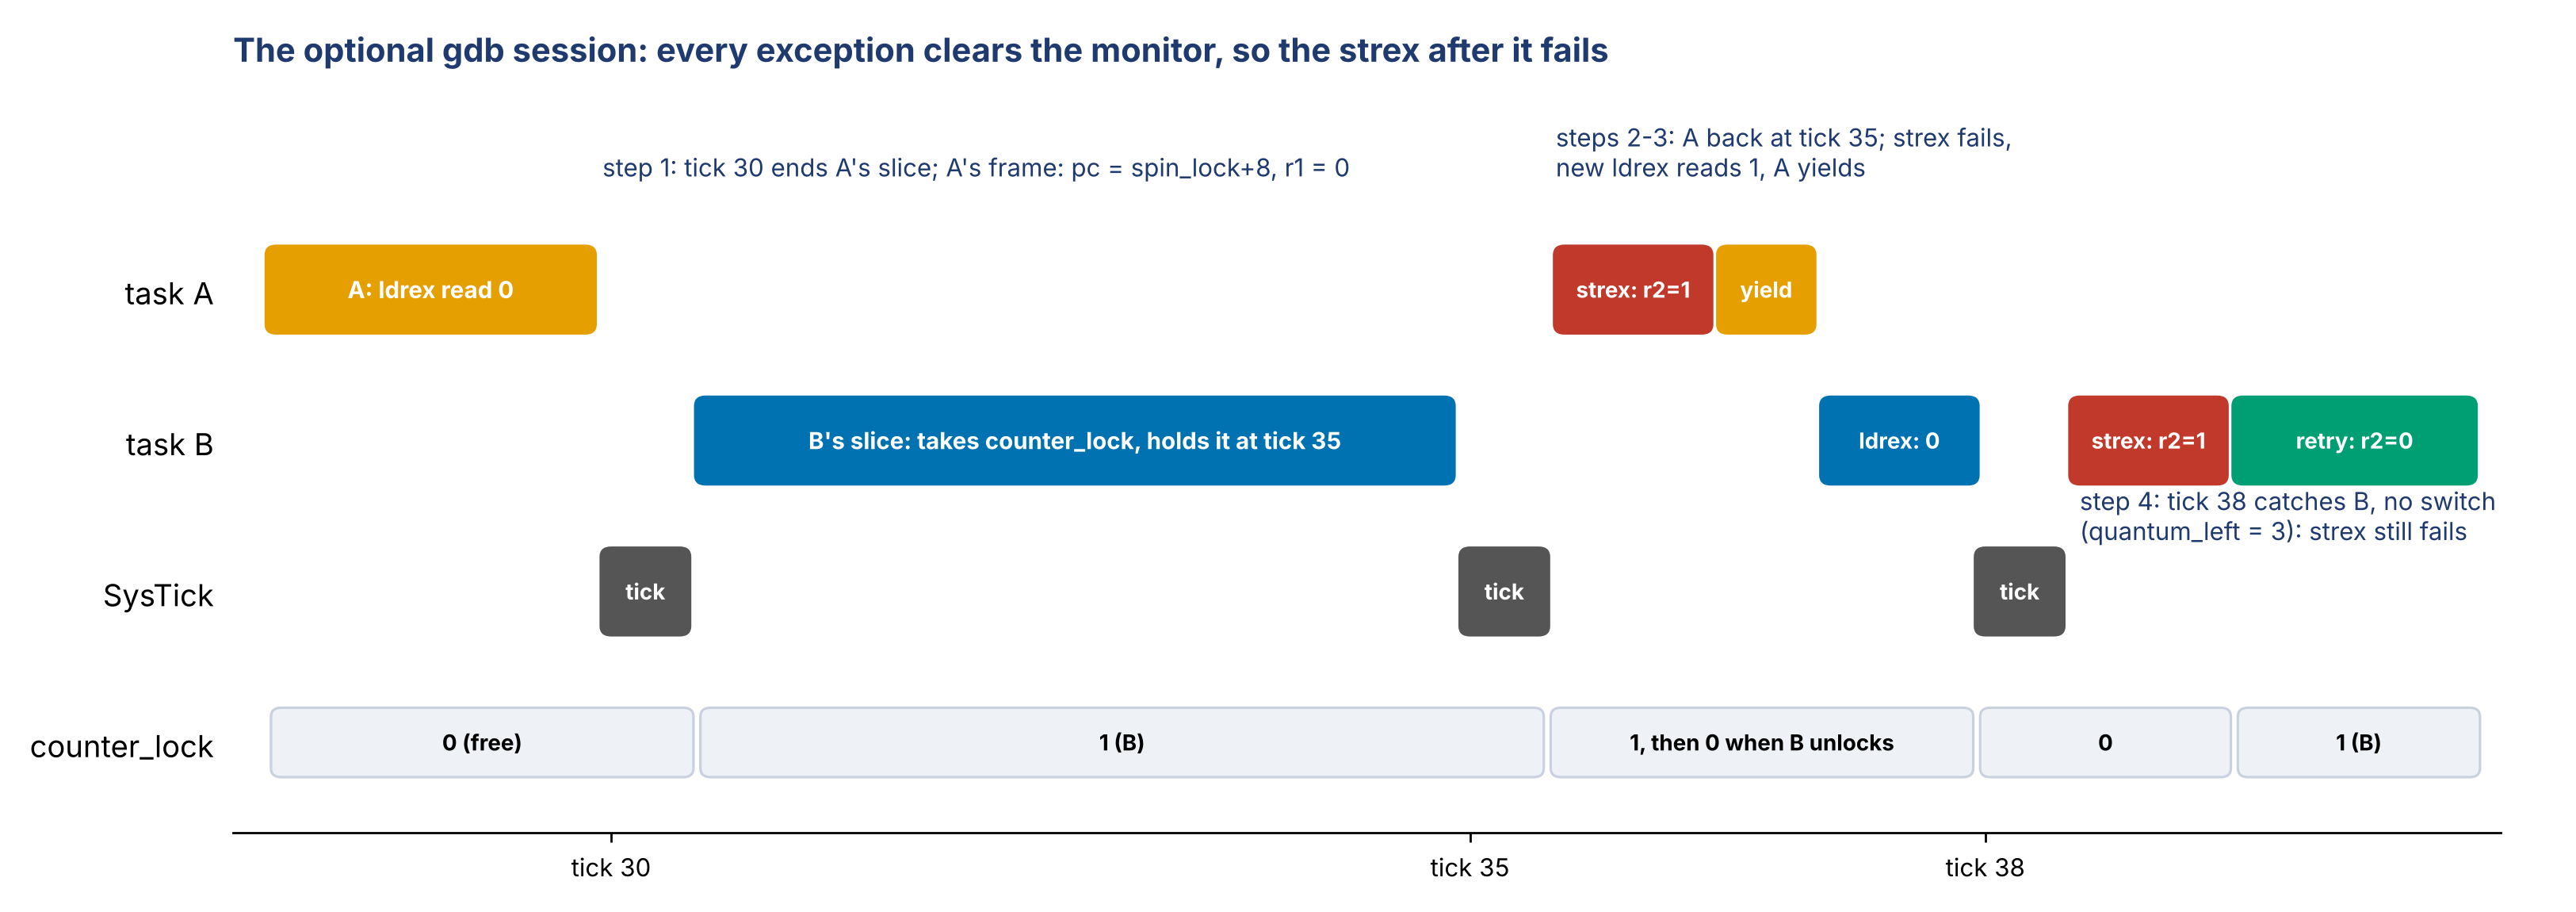
\includegraphics[width=1\textwidth]{contents/images/week-07/gdb_strex_session.png}
    \caption{The whole session on one timeline (schematic, values from the captured run). Step 1 stops A between its \texttt{ldrex} and its \texttt{strex}; B runs a whole slice and holds the lock; back in A the \texttt{strex} fails and A yields. In step 4 a tick that switches nothing still makes B's \texttt{strex} fail, and B's retry succeeds.}
\end{figure}

\paragraph{Step 1: stop on a tick between \texttt{ldrex} and \texttt{strex} that ends the slice.} A \texttt{while} loop in gdb continues from tick to tick until the condition is met (the \texttt{Breakpoint 1, SysTick\_Handler ()} line printed at every skipped tick is left out):
{\verbatimscriptsize
\begin{verbatim}
(gdb) target remote :1234
(gdb) break SysTick_Handler
(gdb) continue
(gdb) while *(unsigned int *)($psp + 24) != (unsigned int) &spin_lock + 8 || quantum_left != 1
 >continue
 >end
(gdb) p tick_count
(gdb) p tcb_current->name
(gdb) x/8wx $psp                                # the interrupted task's frame
(gdb) info symbol *(unsigned int *)($psp + 24)  # the saved pc: word 6
(gdb) p/x counter_lock
(gdb) set $x = tcb_current                      # remember which task it is

Breakpoint 1 at 0xd28: file drivers/systick.c.
$1 = 29
$2 = 0x16fc "A"
0x20000360:     0x20003014      0x00000000      0x000f423f      0x0009928a
0x20000370:     0x00000000      0x00001405      0x0000131c      0x61000000
spin_lock + 8 in section .text
$3 = 0x0
\end{verbatim}}
The 30th tick caught \textbf{A}. In its frame: \texttt{r0 = 0x20003014} (\texttt{\&counter\_lock}), \texttt{r1 = 0} (the lock was free), \texttt{lr = 0x1405} (back into \texttt{task\_a}), \texttt{pc = 0x131c} $=$ \texttt{spin\_lock + 8}, \texttt{xPSR = 0x61000000} (T bit, plus Z and C from \texttt{cmp r1, \#0}); \texttt{r2}, \texttt{r3} are leftovers. \texttt{counter\_lock} is 0: A was one instruction away from the lock.

\paragraph{Step 2: let the other task run, and stop when A is switched back in.} \texttt{PendSV\_Handler + 18} is the instruction right after \texttt{bl task\_switch\_context} in \texttt{kernel/pendsv.s}: there \texttt{tcb\_current} is already the \textbf{new} task.
{\verbatimscriptsize
\begin{verbatim}
(gdb) delete
(gdb) break *PendSV_Handler+18
(gdb) continue
(gdb) p tcb_current->name
(gdb) while tcb_current != $x
 >continue
 >end
(gdb) p tick_count
(gdb) p/x counter_lock

Breakpoint 2 at 0xcc2: file kernel/pendsv.s.
Breakpoint 2, PendSV_Handler () at kernel/pendsv.s
$4 = 0x1700 "B"
Breakpoint 2, PendSV_Handler () at kernel/pendsv.s
$5 = 35
$6 = 0x1
\end{verbatim}}
B ran its whole slice (ticks 30 to 35) and A is back at tick 35. \texttt{counter\_lock} is now \textbf{1}: B took the lock and still held it when its slice ended, the ``almost every time'' case of the \texttt{DEMO=spin} trace.

\paragraph{Step 3: watch A's \texttt{strex} fail.} A resumes at \texttt{mov r1, \#1}, with the \texttt{r1 = 0} it read before the switch. Stop it right after its \texttt{strex}:
{\verbatimscriptsize
\begin{verbatim}
(gdb) delete
(gdb) break *spin_lock+16
(gdb) continue
(gdb) p $r2
(gdb) p/x counter_lock
(gdb) stepi 3
(gdb) p $r1
(gdb) stepi 5

Breakpoint 3 at 0x1324: file lib/spinlock.s.
Breakpoint 3, spin_lock () at lib/spinlock.s
$7 = 1
$8 = 0x1
spin_lock () at lib/spinlock.s
$9 = 1
SVC_Handler () at kernel/svc_entry.s
\end{verbatim}}
\texttt{r2 = 1}: the \texttt{strex} \textbf{failed}, and \texttt{counter\_lock} is still B's 1, although A's \texttt{r1} said ``free''. \texttt{stepi 3} (\texttt{cmp}, \texttt{bne}, the new \texttt{ldrex}) gives \texttt{r1 = 1}; \texttt{stepi 5} reaches the \texttt{svc \#6} of \texttt{task\_yield}: A yields to the holder. These are answers 1 to 3 of the exercise, on a real run.

\paragraph{Step 4 (same session): a tick that switches nothing.} Now a tick that falls between \texttt{ldrex} and \texttt{strex} but does \textbf{not} end the slice (\texttt{quantum\_left} is not 1), as in answer 4:
{\verbatimscriptsize
\begin{verbatim}
(gdb) delete
(gdb) break SysTick_Handler
(gdb) continue
(gdb) while *(unsigned int *)($psp + 24) != (unsigned int) &spin_lock + 8 || quantum_left == 1
 >continue
 >end
(gdb) p tick_count
(gdb) p quantum_left
(gdb) p tcb_current->name
(gdb) delete
(gdb) break *spin_lock+16
(gdb) continue
(gdb) p $r2
(gdb) p/x counter_lock
(gdb) continue
(gdb) p $r2
(gdb) p/x counter_lock

Breakpoint 4 at 0xd28: file drivers/systick.c.
$10 = 37
$11 = 3
$12 = 0x1700 "B"
Breakpoint 5 at 0x1324: file lib/spinlock.s.
Breakpoint 5, spin_lock () at lib/spinlock.s
$13 = 1
$14 = 0x0
Breakpoint 5, spin_lock () at lib/spinlock.s
$15 = 0
$16 = 0x1
\end{verbatim}}
The tick caught \textbf{B} with 3 ticks left in its slice: no switch. B's \texttt{strex} still \textbf{fails} (\texttt{r2 = 1}, \texttt{counter\_lock} stays 0): the tick alone cleared the monitor. At the retry \texttt{r2 = 0} and the lock is 1: B holds it one round later (answer 4). Quit gdb with \texttt{quit} (answer \texttt{y}), and QEMU with \texttt{Ctrl-C} in its terminal.

\paragraph{What changes in your own runs.} Tick numbers, which task is caught first, the leftovers in \texttt{r2}/\texttt{r3} and (with another compiler) the addresses. Sometimes the other task frees the lock before its slice ends: then the caught task's \texttt{strex} still fails, but its retry takes the lock at once. What never changes: \texttt{pc = spin\_lock + 8}, \texttt{r1 = 0}, and \texttt{r2 = 1} for the \texttt{strex} right after the tick.

\section{Unit 2: summary}
\begin{itemize}
    \item The tasks share data only in the \textbf{shared region}: the \texttt{NOLOAD} section \texttt{.shared} at \texttt{0x20003000}, 1\,KB, opened to both tasks by MPU region 2, which never changes on a switch. Its variables start at 0, so its locks start free.
    \item \texttt{spin\_lock\_busy} takes the lock with \texttt{ldrex}, \texttt{cmp}, \texttt{bne}, \texttt{mov}, \texttt{strex} and a retry, then \texttt{dmb}; \texttt{spin\_unlock} is \texttt{dmb} and a plain store of 0. This code is CPU-specific: it must be rewritten for every port of the OS.
    \item A task preempted between \texttt{ldrex} and \texttt{strex} fails its \texttt{strex} and retries: every exception clears the monitor, so the kernel needs no \texttt{clrex}.
    \item \texttt{dmb} is a checkpoint on memory operations: needed on complex or multi-core CPUs, almost free on the M3; it throws away the hardware optimisations, so it goes only where order matters, as in a lock.
    \item With the lock, \texttt{counter=2000000} and every line is whole. Busy waiting costs whole slots, which the trace shows only as a late finish: about 259 ticks on average.
    \item \texttt{spin\_lock} calls \texttt{task\_yield} while the lock is taken, saving \texttt{r0} and \texttt{lr} (AAPCS, 8-byte alignment: always an even number of registers): the waiter's slots shrink to 0 ticks, and the run ends at about 171.
    \item A spinlock gives mutual exclusion and progress, but no fairness; hold it briefly. The scratch-OS stops here by choice: it is the last kernel implementation of the course.
\end{itemize}

\section{Unit 3 - FreeRTOS: the same ideas, a real kernel}
The second lecture of the week moves from writing the scratch-OS to \textbf{using FreeRTOS}: enough to create a few tasks in next week's lab, and, more important, the scratch-OS and FreeRTOS \textbf{side by side}. Most of what we built is exactly the same in FreeRTOS; one thing our kernel has and this FreeRTOS port does not is the memory protection of week 4. FreeRTOS is bigger, more organised and has more features, but we are not that far.

In this unit, file paths are relative to \texttt{freertos-labs/week-07/solution/}, except the kernel files, which are written \texttt{FreeRTOS/Source/...} and are relative to \texttt{freertos-labs/}. You work in \texttt{freertos-labs/week-07/base/}.

\subsection{FreeRTOS: a real kernel on your board}
FreeRTOS is a small real-time kernel: tasks, a scheduler driven by a tick, delays, and tools for tasks that share data. It is written in C, with a few lines of assembly for each CPU family.
\begin{itemize}
    \item It looks very simple, but it is a real \textbf{commercial product}, used in industry in millions of small devices (sensors, cars, home devices): you probably do not see it, but it is very widespread.
    \item Its \textbf{MIT licence}, one of the licences for distributing open-source software and a very easy one, lets anyone take the product, embed it in their own product for commercial use, without any problem, and even change it.
    \item An operating system must be written for a specific CPU and for a specific board, because the I/O devices count. FreeRTOS has been ported to many CPUs and many boards: if you build a small embedded system on a commercial board, it is very likely supported. It runs on the same board as the scratch-OS (the MPS2-AN385, a Cortex-M3), one of the supported ones, and in the same QEMU: the boot, the vector table, SysTick and PendSV are the ones you know.
    \item The part of the kernel that depends on the CPU is called the \textbf{port}. This course uses the \texttt{ARM\_CM3} port, written for the Cortex-M3, in \texttt{FreeRTOS/Source/portable/GCC/ARM\_CM3/}.
    \item What changes for you: in weeks 2--5 (the first six weeks of the course) you worked both on application tasks and on the kernel. From now on the kernel is given, and \textbf{frozen}: you write the tasks, i.e.\ application code.
    \item You never edit the kernel. You can read it, as in the next subsections: most of it will look familiar, because you built the same mechanisms yourself.
\end{itemize}

\subsection{Inspect: the week-07 folder}
The work moves to a \textbf{new repository} on the Git server, \texttt{freertos-labs/}, next to \texttt{scratch-os/}, which will not be touched any more. (The name is misleading: these are not the labs of Monday and Thursday, but the code used in the lectures from now on.) This week's starting point is \texttt{freertos-labs/week-07/base/}:
{\verbatimscriptsize
\begin{verbatim}
freertos-labs/
|-- FreeRTOS/Source/        the kernel: tasks.c, list.c, queue.c, include/, portable/
`-- week-07/base/
    |-- Makefile            APP ?= hello: builds apps/$(APP).c + bsp/*.c + the kernel files
    |-- FreeRTOSConfig.h    the kernel settings for this course (next subsection)
    |-- apps/               hello.c, periodic.c, starve.c: one program each, main() is written
    `-- bsp/                board support: startup.c, mps2_m3.ld, uart.c, syscalls.c,
                            console.c, hooks.c
\end{verbatim}}
\begin{itemize}
    \item \textbf{\texttt{FreeRTOS/}} is the kernel as downloaded from the FreeRTOS repository: the \textbf{source code} plus a \textbf{demo} folder. \textbf{Stay with this version} (chosen in August): FreeRTOS sometimes makes changes that break applications written for the previous one.
    \item As with the scratch-OS, every week has a \textbf{base} and a \textbf{solution} folder. But the scratch-OS was copied every week with more features, while FreeRTOS lives in \textbf{one} folder, never touched, which every week's \texttt{Makefile} compiles from \texttt{../../FreeRTOS/Source}. Your code goes only in \texttt{apps/}.
    \item \textbf{\texttt{FreeRTOSConfig.h}}, in every folder: every feature that can be enabled, disabled or sized is a define in this file; to change the final image of the OS you work only here (next subsection).
    \item \textbf{\texttt{bsp/}}: FreeRTOS includes \textbf{no device drivers}. The board vendor gives them as a \textbf{BSP} (\textbf{board support package}): here mainly the UART driver and the few functions the applications need. The layout is not mandatory, but it is used almost everywhere.
\end{itemize}

\paragraph{The \texttt{Makefile}, closer.}
\begin{itemize}
    \item \texttt{KERNEL := ../../FreeRTOS/Source}: the kernel is compiled from the shared folder, \textbf{never copied}.
    \item The kernel files built are \texttt{tasks.c} (tasks and scheduler), \texttt{list.c} (the lists the scheduler uses), \texttt{queue.c}, \texttt{timers.c}, the port \texttt{portable/GCC/ARM\_CM3/port.c}, and \texttt{portable/MemMang/heap\_4.c}, the heap.
    \item \texttt{APP ?= hello} chooses the program: \texttt{apps/\$(APP).c} is compiled together with every file of \texttt{bsp/}. Each program gets its own build folder and its own \texttt{build/<app>.elf}, so switching programs never needs \texttt{make clean}.
    \item The C library is newlib-nano (\texttt{-specs=nano.specs -lc -lgcc}), so the programs can use \texttt{vsnprintf}.
    \item \texttt{make run} runs \texttt{qemu-system-arm -machine mps2-an385 -monitor null -nographic -serial stdio -kernel build/<app>.elf}, the same command as for the scratch-OS; \texttt{make debug} adds \texttt{-s -S}: QEMU waits frozen for gdb on port 1234. \texttt{DEMO=fixed} is an option used only by \texttt{APP=starve}.
\end{itemize}
The slide asks three questions. \emph{Which file do you change to build another program?} None: you choose the program with \texttt{APP} (\texttt{make APP=periodic}), and edit only the files in \texttt{apps/}. \emph{Why is the kernel path relative, not absolute?} The course folder name contains spaces, which would break an absolute path in the compiler flags (\texttt{-I/path with spaces/...} is cut at the first space). \emph{Why is it good that the kernel is not copied?} One shared copy means every week uses the same kernel, and nobody can change it by mistake.

\paragraph{The board support, \texttt{bsp/}.} It plays the role of \texttt{boot/} and \texttt{drivers/} in the scratch-OS:
\begin{itemize}
    \item \texttt{bsp/startup.c}: \texttt{Reset\_Handler} sets the stack pointer, copies \texttt{.data} from FLASH to RAM and zeroes \texttt{.bss}, as your \texttt{boot/startup.s} did, then calls \texttt{board\_start}, which starts the UART and calls \texttt{main()}. The vector table \texttt{isr\_vector} puts the three handlers of the FreeRTOS port in the SVCall, PendSV and SysTick slots: \texttt{vPortSVCHandler}, \texttt{xPortPendSVHandler} and \texttt{xPortSysTickHandler}.
    \item \texttt{bsp/mps2\_m3.ld}: the linker script, FLASH at \texttt{0x00000000} and RAM at \texttt{0x20000000}.
    \item \texttt{bsp/uart.c}: UART0 driven directly with the CMSDK registers, as in week 3. \texttt{uart\_putc} waits while the transmit buffer is full, then writes the byte; \texttt{uart\_write} sends the bytes one by one. There is no interrupt and no ring: the CPU waits for the UART.
    \item \texttt{bsp/syscalls.c}: the small functions the C library needs. \texttt{\_write} sends everything to UART0; \texttt{\_fstat} says that the output is a character device (\texttt{S\_IFCHR}) and \texttt{\_isatty} returns 1, so the C library treats the output like a terminal; the other functions are stubs. There is no semihosting: all output goes through the UART.
    \item \texttt{bsp/console.c}: \texttt{console\_print}, the \texttt{printf} for tasks (see below).
    \item \texttt{bsp/hooks.c}: the functions the kernel calls when something goes wrong. Each one masks interrupts, prints a message straight to the UART and stops:
    \begin{itemize}
        \item \texttt{vAssertCalled} (a failed \texttt{configASSERT});
        \item \texttt{vApplicationStackOverflowHook} (a stack overflow);
        \item \texttt{vApplicationMallocFailedHook} (the heap is full).
    \end{itemize}
\end{itemize}

\subsection{Inspect: \texttt{FreeRTOSConfig.h}}
The kernel reads this file to decide which features to build and how big its tables are. It contains only \textbf{defines}: every parameter of the FreeRTOS code is tied to a define, and the kernel is full of \textbf{conditional preprocessing}. A line such as \texttt{\#ifdef SYMBOL} in the source is a conditional statement for the preprocessor: if the symbol is defined somewhere, the block is included in the code; otherwise it is skipped. The options that matter today (values from the file, comments shortened):
\begin{lstlisting}[language=C, showstringspaces=false, basicstyle=\ttfamily\scriptsize]
#define configUSE_PREEMPTION            1      /* a more urgent READY task takes the CPU at once */
#define configUSE_TIME_SLICING          1      /* equal priorities take turns, one tick each */
#define configMAX_PRIORITIES            ( 5 )  /* priorities 0 (idle task) to 4; higher = more urgent */
#define configCPU_CLOCK_HZ              ( ( unsigned long ) 25000000 )   /* 25 MHz */
#define configTICK_RATE_HZ              ( ( TickType_t ) 100 )           /* 100 ticks per second */
#define configMINIMAL_STACK_SIZE        ( ( unsigned short ) 256 )       /* in WORDS */
#define configTOTAL_HEAP_SIZE           ( ( size_t ) ( 64 * 1024 ) )     /* bytes */
#define configCHECK_FOR_STACK_OVERFLOW  2      /* check the stack at every switch */
#define configASSERT( x )    if( ( x ) == 0 ) vAssertCalled( __FILE__, __LINE__ )
\end{lstlisting}
\begin{center}
\footnotesize
\begin{tabular}{P{0.43} P{0.49}}
    \hline
    \textbf{define (value)} & \textbf{meaning} \\
    \hline
    \texttt{configUSE\_PREEMPTION} (1) & a more urgent READY task takes the CPU at once. Not a run-time switch: it includes or leaves out the code of preemption (conditional preprocessing) \\
    \texttt{configUSE\_TIME\_SLICING} (1) & tasks of the \textbf{same} priority share the CPU in round robin, one tick each \\
    \texttt{configMAX\_PRIORITIES} (5) & priorities 0--4: the kernel creates one ready list per priority \\
    \texttt{configCPU\_CLOCK\_HZ} (25\,MHz) & the board's clock, needed to program the timers at start-up \\
    \texttt{configTICK\_RATE\_HZ} (100) & a \textbf{frequency}, not a period: 100 ticks/s $=$ 10\,ms, the scratch-OS tick; \texttt{TickType\_t} is 32 bits \\
    \texttt{configMINIMAL\_STACK\_SIZE} (256) & in \textbf{words}: 1\,KB; used for the tasks the kernel creates itself (the idle task) \\
    \texttt{configTOTAL\_HEAP\_SIZE} (64\,KB) & FreeRTOS has \textbf{dynamic memory}: TCBs and stacks come from this heap (\texttt{heap\_4.c}); our stacks were fixed partitions \\
    \texttt{configCHECK\_FOR\_STACK\_OVERFLOW} (2),\newline \texttt{configASSERT} & self-checks: \texttt{vAssertCalled} and \texttt{vApplicationStackOverflowHook} in \texttt{bsp/hooks.c} print and stop \\
    \texttt{configKERNEL\_INTERRUPT\_PRIORITY} (255),\newline \texttt{configMAX\_SYSCALL\_INTERRUPT\_PRIORITY} (191) & the kernel's interrupt priorities, used with BASEPRI (below) \\
    \hline
\end{tabular}
\end{center}
Other switches mentioned in class: \texttt{configUSE\_PORT\_OPTIMISED\_TASK\_SELECTION} (a portable C task selection, or a faster one written by the port: ``here is a version supported everywhere; if you want performance, write your own''), \texttt{configIDLE\_SHOULD\_YIELD} (1: the idle task yields at once to other priority-0 tasks), \texttt{configMAX\_TASK\_NAME\_LEN} (saving 10 bytes matters on a tiny system) and \texttt{configSUPPORT\_DYNAMIC\_ALLOCATION} (the course uses dynamic memory, because everything is simpler). There are about 200 switches: the documentation is the only way to know them all.

\paragraph{Hooks.} Many definitions end with \texttt{HOOK}. FreeRTOS is not extended by editing the kernel: at the points that may need an extension, the kernel calls an external \textbf{hook function} that \emph{you} define, if its switch is on. For example, with \texttt{configUSE\_IDLE\_HOOK} (0 here) the idle task does its mandatory work and then calls your \texttt{vApplicationIdleHook}. The message: \textbf{never touch the FreeRTOS kernel}; work only with hook functions.

\subsection{Try it: build and run}
Goal: build the kernel and one program, and see the board boot. Building and running is very simple, with a Makefile taken from the FreeRTOS demos; the only difference is that it needs a parameter, the \textbf{name of the app} to build, so that one week's folder can hold more than one app. In the base every task body is still empty: it only parks the task with \texttt{vTaskSuspend( NULL )}.
\begin{lstlisting}[language=bash]
    cd freertos-labs/week-07/base
    make APP=hello run
\end{lstlisting}
What you see (the compiler lines and the link line are left out):
{\verbatimscriptsize
\begin{verbatim}
qemu-system-arm -machine mps2-an385 -monitor null -nographic -serial stdio -kernel build/hello.elf
hello: FreeRTOS on the MPS2-AN385, tick = 10 ms
\end{verbatim}}
\begin{itemize}
    \item Only \texttt{main()}'s banner appears, printed at the beginning of \texttt{main}, even before the scheduler starts, with a summary of the parameters: FreeRTOS, the board, the tick. The tasks do nothing yet.
    \item QEMU keeps running: stop it with \texttt{Ctrl-C} (if that does not work: \texttt{Ctrl-A}, release, then \texttt{X}).
    \item \texttt{make APP=periodic run} and \texttt{make APP=starve run} print their own banners in the same way.
\end{itemize}

\subsection{Your kernel and FreeRTOS, side by side}
\begin{figure}[H]
\centering
\resizebox{\textwidth}{!}{%
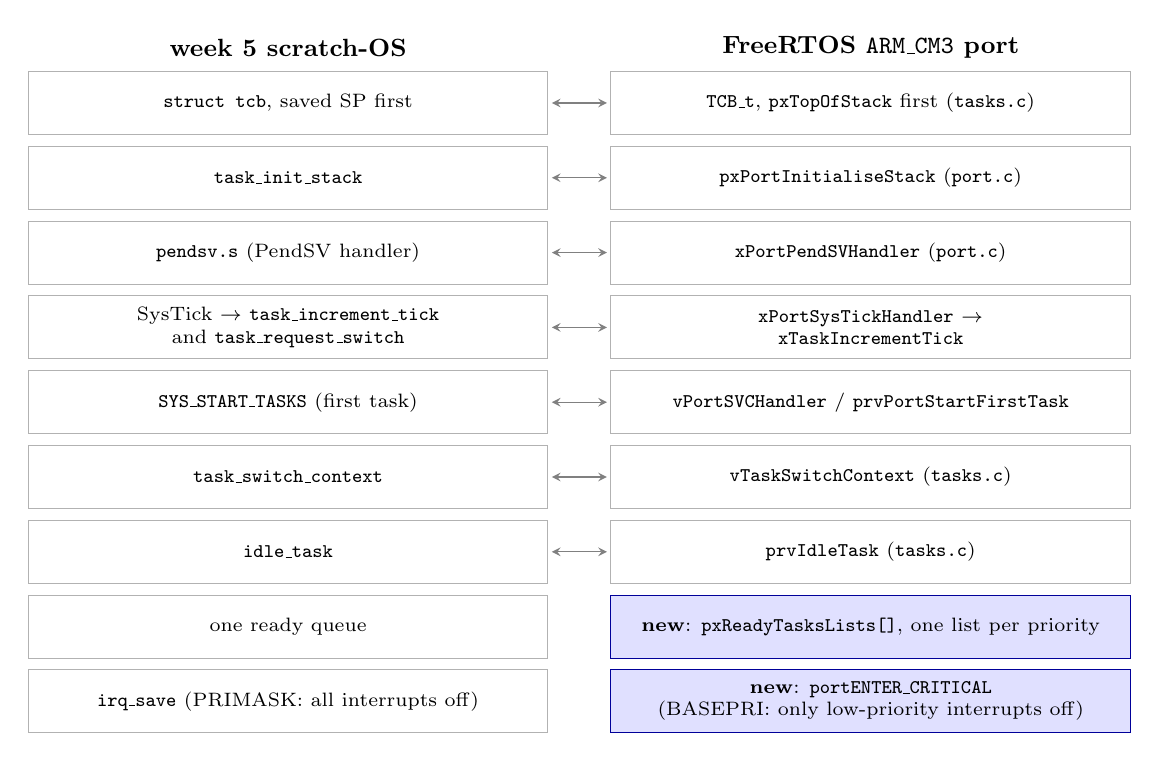
\begin{tikzpicture}[font=\scriptsize,
    c/.style={draw=gray!60, minimum width=6.6cm, minimum height=0.8cm, align=center, inner sep=2pt},
    n/.style={c, fill=blue!12, draw=blue!60!black}]
    \node[font=\small\bfseries] at (0,0.7) {week 5 scratch-OS};
    \node[font=\small\bfseries] at (7.4,0.7) {FreeRTOS \texttt{ARM\_CM3} port};
    \foreach \l/\r [count=\i from 0] in {
        {\texttt{struct tcb}, saved SP first}/{\texttt{TCB\_t}, \texttt{pxTopOfStack} first (\texttt{tasks.c})},
        {\texttt{task\_init\_stack}}/{\texttt{pxPortInitialiseStack} (\texttt{port.c})},
        {\texttt{pendsv.s} (PendSV handler)}/{\texttt{xPortPendSVHandler} (\texttt{port.c})},
        {SysTick $\to$ \texttt{task\_increment\_tick}\\and \texttt{task\_request\_switch}}/{\texttt{xPortSysTickHandler} $\to$\\\texttt{xTaskIncrementTick}},
        {\texttt{SYS\_START\_TASKS} (first task)}/{\texttt{vPortSVCHandler} / \texttt{prvPortStartFirstTask}},
        {\texttt{task\_switch\_context}}/{\texttt{vTaskSwitchContext} (\texttt{tasks.c})},
        {\texttt{idle\_task}}/{\texttt{prvIdleTask} (\texttt{tasks.c})}} {
        \node[c] at (0,-0.95*\i) {\l};
        \node[c] at (7.4,-0.95*\i) {\r};
        \draw[gray, <->, >=stealth] (3.35,-0.95*\i) -- (4.05,-0.95*\i);
    }
    \node[c] at (0,-6.65) {one ready queue};
    \node[n] at (7.4,-6.65) {\textbf{new}: \texttt{pxReadyTasksLists[]}, one list per priority};
    \node[c] at (0,-7.6) {\texttt{irq\_save} (PRIMASK: all interrupts off)};
    \node[n] at (7.4,-7.6) {\textbf{new}: \texttt{portENTER\_CRITICAL}\\(BASEPRI: only low-priority interrupts off)};
\end{tikzpicture}}
\caption{The scratch-OS and FreeRTOS side by side. Every mechanism on the left is one you built; white rows are the same feature with different names, the two blue rows are the new ideas.}
\end{figure}
Most rows are white: the same feature, our OS is not that different.
\begin{itemize}
    \item Both have a data structure for the \textbf{task control block}, with different names: \texttt{struct tcb} in our OS, the type \texttt{TCB\_t} in FreeRTOS.
    \item Both have a function that, when a task is created, initialises its stack with the words that let the exception return perform the switch: \texttt{task\_init\_stack} in our OS, \texttt{pxPortInitialiseStack} in FreeRTOS.
    \item The switch is done with the \textbf{PendSV} exception, the common way to implement it on an ARM processor: FreeRTOS does exactly the same. It also starts the first task by \textbf{faking an exception}, as we did, and the switch between two tasks is very similar.
    \item Both have an \textbf{idle task}.
\end{itemize}
The differences, in blue:
\begin{itemize}
    \item \textbf{The scheduler}: ours has only one priority and only one ready queue; FreeRTOS is priority-based, with \textbf{many ready queues}.
    \item \textbf{Critical sections}: in some portions of our scheduler we masked \emph{all} interrupts, so as not to be interrupted, then enabled them again. FreeRTOS uses a better approach: it masks only the interrupts with a lower priority than the code doing the switch, so that something really important, more important than scheduling, is still handled.
\end{itemize}
The next subsections open the right column, from screenshots of the FreeRTOS code; the comments on them are \textbf{the professor's}, not those of the source code, written to explain what matters in class.

\subsection{Inspect: \texttt{TCB\_t} in \texttt{FreeRTOS/Source/tasks.c}}
Look for \texttt{typedef struct tskTaskControlBlock}. Its first fields (comments ours):
\begin{lstlisting}[language=C, showstringspaces=false, basicstyle=\ttfamily\scriptsize]
typedef struct tskTaskControlBlock
{
    volatile StackType_t * pxTopOfStack; /* saved SP: "MUST BE THE FIRST MEMBER" */
    ListItem_t xStateListItem;            /* links the task into ONE state list */
    ListItem_t xEventListItem;            /* used when a task waits for an event */
    UBaseType_t uxPriority;               /* 0 = lowest (the idle task) */
    StackType_t * pxStack;                /* lowest address of the stack */
    char pcTaskName[ configMAX_TASK_NAME_LEN ];
    /* ... more fields, each one switched on by a config option ... */
} tskTCB;
typedef tskTCB TCB_t;
\end{lstlisting}
\begin{itemize}
    \item Very similar to ours. The \textbf{top of the stack} is saved as the \textbf{first} element, for the same reason: when the exception that switches tasks runs, it needs this information to find where the task's stack is.
    \item \texttt{pxCurrentTCB}, declared a few lines below, is your \texttt{tcb\_current}: the TCB of the task that runs.
    \item \textbf{No state field}: the state is the \textbf{list} the task is in (below). Linked lists are natural with dynamic memory; with static memory they would be a nightmare.
    \item \texttt{uxPriority}: as in our TCB, the priority.
    \item \texttt{pxStack}: very important. FreeRTOS saves the stack pointer, but also the \textbf{bottom} of the stack, because one feature that can be enabled is the detection of a \textbf{stack overflow}, usually done at the context switch. To detect it you need to know where the stack is and how big: if it grows too much, it overflows (and popping too much would go past the other end)\footnote{In FreeRTOS the check of \texttt{configCHECK\_FOR\_STACK\_OVERFLOW} looks at the end towards which the stack grows: on the Cortex-M the stack grows downwards, so the limit is \texttt{pxStack}, its lowest address.}. So both pieces of information are in the TCB.
    \item Then the task name, and many other fields.
\end{itemize}

\paragraph{FreeRTOS naming.} Variables and functions start with \texttt{px}, \texttt{x}, \texttt{ux}, \dots: FreeRTOS names variables after their \textbf{data type}. Not for the exam, but if one day you work for a company that uses FreeRTOS you need to understand it, and code written for FreeRTOS should respect it.
\begin{itemize}
    \item \textbf{Variables}: the first letters give the type. \texttt{px} = pointer, \texttt{ux} = unsigned, \texttt{x} = any other type (a float, a structure, \dots), \texttt{pc} = pointer to char (\texttt{x} is often \texttt{BaseType\_t} or a struct).
    \item \textbf{Functions}: the prefix is the type of the \textbf{return value}: \texttt{v} = the function returns \texttt{void}, \texttt{x} = it returns a value. \texttt{prv} = private to its file. So \texttt{pxTopOfStack} is a pointer, \texttt{uxPriority} an unsigned number, and \texttt{prvIdleTask} a function you cannot call from outside \texttt{tasks.c}.
    \item It is only a convention, to understand code easily: code that ignores it works all the same (and the professor does not guarantee that all his code respects it).
\end{itemize}

\subsection{The port: \texttt{portable/}}
FreeRTOS is built from a \textbf{portable} part and a \textbf{machine-dependent} part. The machine-dependent code is in the folder \texttt{FreeRTOS/Source/portable/}, and there everything becomes complex: every CPU is different, but the code also depends on the \textbf{toolchain} used to compile it. Even on an ARM processor, building with GCC or with the ARM compiler gives different code. So FreeRTOS provides ports for different toolchains, and, for each toolchain, for different machines.
\begin{itemize}
    \item We compile with GCC, so the port is under \texttt{portable/GCC/}: what is there works only with GCC.
    \item Inside, one folder per CPU (or board) that FreeRTOS supports. Many are ARM, not surprising: ARM is one of the most used CPUs in embedded designs today. But there are other CPUs too, e.g.\ a processor by Xilinx (AMD) for reconfigurable boards.
    \item Ours is \texttt{ARM\_CM3}, for the Cortex-M3. It holds only two files: \texttt{port.c} and its include file, \texttt{portmacro.h}, with all the code specific to porting FreeRTOS to that machine.
    \item The root of \texttt{FreeRTOS/Source} holds the kernel proper: \texttt{tasks.c}, \texttt{timers.c}, \texttt{queue.c}, \texttt{stream\_buffer.c}, \texttt{event\_groups.c}, \texttt{croutine.c}. For example \texttt{tasks.c} contains the scheduler and the functions that create tasks. These files are \textbf{machine-independent}: they use functions defined in a \texttt{port.c}, which are machine-dependent.
    \item The build takes those functions from the port folder of the chosen CPU; on another CPU you change that folder. It is not magic, and FreeRTOS does not choose by itself: the \textbf{Makefile} chooses the platform. FreeRTOS's own build files have a variable where you write the platform you want; the course Makefile uses them.
\end{itemize}

\subsection{Inspect: \texttt{pxPortInitialiseStack} in \texttt{ARM\_CM3/port.c}}
File \texttt{FreeRTOS/Source/portable/GCC/ARM\_CM3/port.c}. \texttt{xTaskCreate} calls it once for each new task. Some functions in \texttt{port.c} are very similar to the ones we designed; this one initialises the stack of a task (comments ours):
\begin{lstlisting}[language=C, showstringspaces=false, basicstyle=\ttfamily\scriptsize]
StackType_t * pxPortInitialiseStack( StackType_t * pxTopOfStack, TaskFunction_t pxCode, void * pvParameters )
{
    pxTopOfStack--;
    *pxTopOfStack = portINITIAL_XPSR;                                    /* xPSR = 0x01000000: T bit */
    pxTopOfStack--;
    *pxTopOfStack = ( ( StackType_t ) pxCode ) & portSTART_ADDRESS_MASK; /* PC = task fn */
    pxTopOfStack--;
    *pxTopOfStack = ( StackType_t ) portTASK_RETURN_ADDRESS;             /* LR = prvTaskExitError */
    pxTopOfStack -= 5;                                                   /* skip r12, r3, r2, r1 */
    *pxTopOfStack = ( StackType_t ) pvParameters;                        /* r0 = parameter */
    pxTopOfStack -= 8;                                                   /* room for r11 ... r4 */
    return pxTopOfStack;                                                 /* stored in pxTopOfStack */
}
\end{lstlisting}
Our \texttt{task\_init\_stack} does exactly the same, in the same order: it must, because the switch is an exception return and the CPU pops the frame by itself. 8 words of fake hardware frame (xPSR, PC, LR, \texttt{r12}, \texttt{r3}--\texttt{r0}) plus 8 words for \texttt{r4}--\texttt{r11}; the new element is the \textbf{task parameter} in \texttt{r0}. The PC has bit 0 cleared; the T bit in xPSR says ``Thumb''.

\begin{figure}[H]
\centering
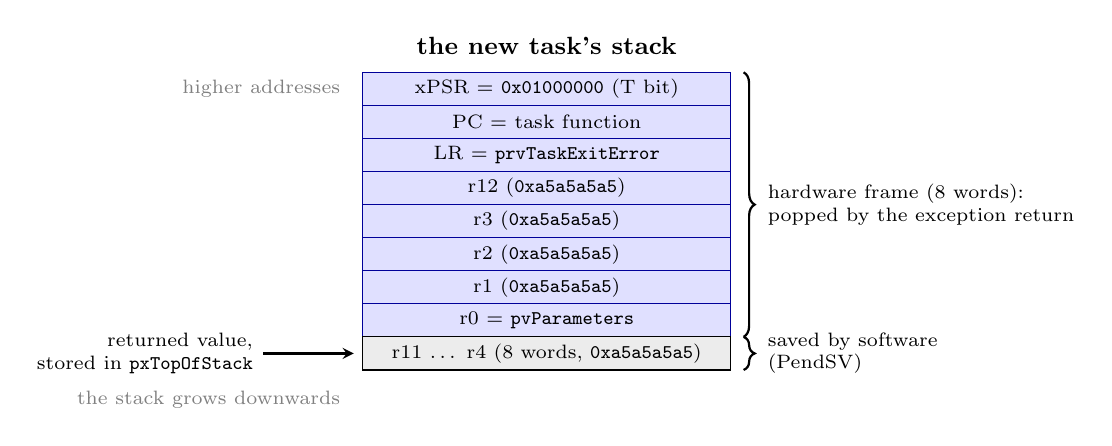
\begin{tikzpicture}[font=\scriptsize,
    w/.style={draw, text width=4.6cm, minimum height=0.42cm, align=center, inner sep=1pt},
    hw/.style={w, fill=blue!12, draw=blue!60!black},
    sw/.style={w, fill=gray!15}]
    \node[font=\small\bfseries] at (0,0.55) {the new task's stack};
    \foreach \t/\st [count=\i from 0] in {
        {xPSR = \texttt{0x01000000} (T bit)}/hw, {PC = task function}/hw, {LR = \texttt{prvTaskExitError}}/hw,
        {r12 (\texttt{0xa5a5a5a5})}/hw, {r3 (\texttt{0xa5a5a5a5})}/hw, {r2 (\texttt{0xa5a5a5a5})}/hw, {r1 (\texttt{0xa5a5a5a5})}/hw,
        {r0 = \texttt{pvParameters}}/hw,
        {r11 \dots\ r4 (8 words, \texttt{0xa5a5a5a5})}/sw} {
        \node[\st] at (0,-0.42*\i) {\t};
    }
    \draw[decorate, decoration={brace, amplitude=4pt}, thick] (2.5,0.21) -- node[right=5pt, align=left] {hardware frame (8 words):\\popped by the exception return} (2.5,-3.15);
    \draw[decorate, decoration={brace, amplitude=4pt}, thick] (2.5,-3.15) -- node[right=5pt, align=left] {saved by software\\(PendSV)} (2.5,-3.57);
    \draw[->, >=stealth, thick] (-3.6,-3.36) node[left, align=right] {returned value,\\stored in \texttt{pxTopOfStack}} -- (-2.45,-3.36);
    \node[left, align=right, text=gray] at (-2.5,0.0) {higher addresses};
    \node[left, align=right, text=gray] at (-2.5,-3.95) {the stack grows downwards};
\end{tikzpicture}
\caption{The stack prepared by \texttt{pxPortInitialiseStack}, as by our \texttt{task\_init\_stack}: a fake hardware frame of 8 words, plus 8 words for \texttt{r4}--\texttt{r11}, so the first switch to a task is like every other one. The words not written keep the fill value \texttt{0xa5a5a5a5}.}
\end{figure}

\subsection{What \texttt{TCB\_t} and \texttt{pxPortInitialiseStack} show}
\begin{itemize}
    \item \texttt{pxTopOfStack} is your \texttt{sp}, first for the same reason: the switch is written in assembly and reads it at offset 0 (\texttt{ldr r0, [r1]} with \texttt{r1 = pxCurrentTCB}). The kernel's own comment says so in capitals.
    \item \textbf{No state field}: one list per state (ready, delayed, suspended); \texttt{xStateListItem} links the task into one of them, and the list the task is in \textbf{is} its state.
    \item \textbf{No \texttt{wake\_tick} field}: when a task is delayed, FreeRTOS stores its wake-up tick as the value of the task's \texttt{xStateListItem} in the \textbf{delayed list} (a field reused while the task sleeps: a bit dirty, but compact). The delayed list is ordered by these wake-up ticks, so the task due soonest is at the front.
    \item \textbf{No \texttt{tasks[]} table}: \texttt{xTaskCreate} takes the TCB and the stack from the heap with \texttt{pvPortMalloc} (in \texttt{FreeRTOS/Source/portable/MemMang/heap\_4.c}). Your table had a fixed number of tasks; here you can create them as long as the heap has room.
    \item \textbf{\texttt{r0} = parameter}: by the C calling rules, the first argument of a function is in \texttt{r0}. When the hardware pops the fake frame, the task function starts with \texttt{r0 = pvParameters}, exactly as if someone had called \texttt{task( pvParameters )}.
    \item \textbf{Returning}: \texttt{lr = prvTaskExitError}, which makes \texttt{configASSERT} fail on purpose and stops. Your \texttt{task\_exit} let a task finish cleanly; FreeRTOS says a task function must \textbf{never return}.
    \item The skipped words (\texttt{r1}--\texttt{r3}, \texttt{r12}, \texttt{r4}--\texttt{r11}) are not written: they keep the value \texttt{0xa5a5a5a5}, which the kernel writes into every new stack so that it can detect an overflow: if the lowest words of a stack no longer hold the pattern, the task has used them.
\end{itemize}

\subsection{Context switch: save, choose, restore}
FreeRTOS's PendSV handler in \texttt{ARM\_CM3/port.c} handles the context switch in a way almost \textbf{identical} to ours. Read it as three steps: save the old task, choose the next task, restore the new task. It is inline assembly in a \texttt{naked} C function, so there is no compiler-generated code around it (the compiler adds no entry or exit code: the function body is exactly the assembly):
\begin{lstlisting}[basicstyle=\ttfamily\scriptsize]
    mrs r0, psp                  /* sp = PSP: the old task's stack */
    isb                          /* wait until the read is done */
    ldr r3, pxCurrentTCBConst    /* r3 = &pxCurrentTCB */
    ldr r2, [r3]                 /* r2 = pxCurrentTCB */
    stmdb r0!, {r4-r11}          /* sp -= 8; sp[0..7] = r4..r11 */
    str r0, [r2]                 /* pxCurrentTCB->pxTopOfStack = sp */
    stmdb sp!, {r3, r14}         /* push r3 and lr on the main stack (MSP) */
    mov r0, %0                   /* r0 = configMAX_SYSCALL_INTERRUPT_PRIORITY */
    msr basepri, r0              /* BASEPRI = r0: mask the kernel's interrupts */
    bl vTaskSwitchContext        /* vTaskSwitchContext(); changes pxCurrentTCB */
    mov r0, #0
    msr basepri, r0              /* BASEPRI = 0: unmask */
    ldmia sp!, {r3, r14}         /* pop r3 and lr again */
    ldr r1, [r3]                 /* r1 = pxCurrentTCB (the new task) */
    ldr r0, [r1]                 /* sp = pxCurrentTCB->pxTopOfStack */
    ldmia r0!, {r4-r11}          /* r4..r11 = sp[0..7]; sp += 8 */
    msr psp, r0                  /* PSP = sp: points at the hardware frame */
    isb
    bx r14                       /* exception return with the saved EXC_RETURN */
\end{lstlisting}
Save, choose, restore: with different names, the scratch-OS handler. What is \textbf{different} is the choice: we masked \emph{all} interrupts while choosing the next task; FreeRTOS writes \texttt{configMAX\_SYSCALL\_INTERRUPT\_PRIORITY} into \textbf{BASEPRI}, masking only the interrupts below that threshold. An interrupt more important than scheduling (say, an \textbf{alarm} that must shut the system down) is still served; our OS assumed that the scheduler is the most important thing.

\begin{figure}[H]
\centering
\resizebox{\textwidth}{!}{%
\begin{tikzpicture}[font=\scriptsize, >=Stealth]
    \node[font=\small\bfseries] at (4,3.55) {interrupt priorities (Cortex-M: a lower number is more urgent)};
    \fill[green!15] (0,1.7) rectangle (8,3.2);
    \fill[red!12] (0,0) rectangle (8,1.7);
    \draw (0,0) rectangle (8,3.2);
    \draw[very thick, blue!70!black] (-0.3,1.7) -- (8.3,1.7);
    \node[anchor=west, text=blue!70!black, font=\scriptsize\bfseries, align=left] at (8.4,1.7) {BASEPRI = \texttt{configMAX\_SYSCALL\_INTERRUPT\_PRIORITY}\\(while the kernel chooses the next task)};
    \node[align=center] at (4,2.45) {\textbf{more urgent than the threshold}\\still served, e.g.\ an alarm that must shut the system down\\(may not call the kernel)};
    \node[align=center] at (4,0.85) {\textbf{as urgent as the threshold or less}\\masked until BASEPRI = 0\\(SysTick, PendSV, the UART, \dots)};
    \draw[->] (-0.6,0) -- node[left, align=right] {more\\urgent} (-0.6,3.2);
    \node[anchor=west, align=left, text=gray] at (8.4,0.6) {scratch-OS: \texttt{cpsid i} (PRIMASK)\\masks \emph{everything}, alarm included};
\end{tikzpicture}}
\caption{BASEPRI versus PRIMASK. While \texttt{vTaskSwitchContext} runs, FreeRTOS masks only the interrupts at or below the kernel's threshold, chosen in \texttt{FreeRTOSConfig.h}; the more urgent ones are still served. Our kernel masked all of them.}
\end{figure}

\subsection{What the context switch does}
\begin{enumerate}
    \item \textbf{Save the old task}: read its PSP, push \texttt{r4}--\texttt{r11} (everything else was already pushed by the exception), and store the resulting SP in \texttt{pxCurrentTCB->pxTopOfStack}.
    \item \textbf{Choose the next task}: call \texttt{vTaskSwitchContext}. BASEPRI temporarily masks the kernel interrupts, so that they cannot change the ready lists during this decision: this portion must be protected, by masking the interrupts below the threshold.
    \item \textbf{Restore the new task}: read its saved SP, pop \texttt{r4}--\texttt{r11}, write the new PSP, and return from the exception.
\end{enumerate}
The slide asks you to find your 13 instructions in this list, and to name the two additions and why they are needed:
\begin{itemize}
    \item \textbf{The same skeleton}: read PSP (\texttt{mrs r0, psp}), push \texttt{r4}--\texttt{r11} on the old task's stack (\texttt{stmdb r0!}), store the SP at offset 0 of the TCB (\texttt{str r0, [r2]}), call C to choose (\texttt{bl}), load the new SP (\texttt{ldr r0, [r1]}), pop \texttt{r4}--\texttt{r11} (\texttt{ldmia r0!}), write PSP (\texttt{msr psp, r0}), return (\texttt{bx}). Only the names change: \texttt{tcb\_current} $\to$ \texttt{pxCurrentTCB}, \texttt{task\_switch\_context} $\to$ \texttt{vTaskSwitchContext}. Your handler loaded the address of \texttt{tcb\_current} twice; this one loads \texttt{\&pxCurrentTCB} once into \texttt{r3} and keeps it.
    \item \textbf{Addition 1: \texttt{lr} saved on MSP.} \texttt{bl} overwrites \texttt{lr}, which holds the EXC\_RETURN value. Your handler loaded the constant \texttt{0xFFFFFFFD} at the end; FreeRTOS keeps the value it received (here also \texttt{0xFFFFFFFD}) and returns with it. \texttt{r3} is saved too, because the C call may change it, and the handler needs \texttt{\&pxCurrentTCB} after the call.
    \item \textbf{Addition 2: BASEPRI around the C call.} BASEPRI is a Cortex-M register: writing a priority value into it masks the interrupts of that priority and all less urgent ones; 0 masks nothing. In FreeRTOS some interrupt handlers may call the kernel and change its lists, so they must wait while \texttt{vTaskSwitchContext} reads them. In your kernel no handler touched the TCBs during a switch, so nothing needed masking.
    \item \textbf{What is missing}: no MPU region and no CONTROL change (below).
\end{itemize}
\begin{itemize}
    \item \texttt{isb} (instruction synchronization barrier) makes sure a special-register write has taken effect before the next instruction runs.
    \item \textbf{Unlike your scratch-OS}, this port does not change \texttt{CONTROL} or configure an MPU: every FreeRTOS task runs \textbf{privileged} and can access all memory. Here FreeRTOS is ``less good'' than our OS: the base version runs only privileged code, with no memory protection (an MPU can be enabled, with a different port). Several tasks still work, but none of what we had to do to switch between privileged and unprivileged is done.
\end{itemize}

\subsection{Every tick: update time, then request a switch}
Our scratch-OS had a handler for SysTick; FreeRTOS has one too, \texttt{xPortSysTickHandler}. It runs once every 10\,ms. It does not perform the context switch itself; it only decides whether PendSV should do one afterwards:
\begin{lstlisting}[language=C, showstringspaces=false, basicstyle=\ttfamily\scriptsize]
void xPortSysTickHandler( void )
{
    portDISABLE_INTERRUPTS();                           /* protect the kernel's lists */
    {
        if( xTaskIncrementTick() != pdFALSE )           /* advance time; is a switch needed? */
        {
            portNVIC_INT_CTRL_REG = portNVIC_PENDSVSET_BIT;   /* ask PendSV to switch later */
        }
    }
    portENABLE_INTERRUPTS();                            /* BASEPRI = 0 */
}
\end{lstlisting}
\begin{itemize}
    \item It touches the kernel's lists, so it first masks interrupts\footnote{On the Cortex-M3 port, \texttt{portDISABLE\_INTERRUPTS} also works through BASEPRI: it masks the interrupts up to the kernel's threshold, not the more urgent ones, and \texttt{portENABLE\_INTERRUPTS} writes BASEPRI $=$ 0.}.
    \item \textbf{\texttt{xTaskIncrementTick}} (in \texttt{tasks.c}) advances \texttt{xTickCount} (your \texttt{tick\_count}) and compares it with \texttt{xNextTaskUnblockTime}, the wake tick of the \textbf{first} task of the sorted delayed list; the tasks whose time has come move from the delayed list to their ready list.
    \item It returns true when a woken task is \textbf{more urgent} than the running one (\texttt{pxTCB->uxPriority > pxCurrentTCB->uxPriority}), or, with time slicing, when the running task's ready list holds another task. Then the handler sets \textbf{PendSV} pending (the PENDSVSET bit of ICSR, as in your kernel), and PendSV switches when no other handler runs.
    \item Unlike the scratch-OS, the \textbf{tick is the round-robin quantum}: two tasks of the same priority alternate every 10\,ms. We had two parameters (tick and quantum); FreeRTOS thinks in \textbf{priorities}, where two tasks of the same priority should be rare, and if they exist they really run together.
\end{itemize}

\subsection{Starting the first task}
These two routines run once, when \texttt{vTaskStartScheduler()} starts. The first one, \texttt{prvPortStartFirstTask}, resets the main stack and enters SVC; the second one, the SVC handler \texttt{vPortSVCHandler}, loads the first task's saved context and returns into that task:
\begin{lstlisting}[basicstyle=\ttfamily\scriptsize]
/* prvPortStartFirstTask: prepare the CPU */
ldr r0, =0xE000ED08    /* r0 = &VTOR */
ldr r0, [r0]           /* r0 = VTOR: vector table */
ldr r0, [r0]           /* r0 = vector[0]: initial SP */
msr msp, r0            /* MSP = initial SP */
cpsie i                /* enable interrupts */
svc 0                  /* SVCall: start a task */

/* vPortSVCHandler: enter the first task */
ldr r3, pxCurrentTCBConst2   /* r3 = &pxCurrentTCB */
ldr r1, [r3]                 /* r1 = pxCurrentTCB */
ldr r0, [r1]                 /* sp = r1->pxTopOfStack */
ldmia r0!, {r4-r11}          /* r4..r11 = sp[0..7]; sp += 8 */
msr psp, r0                  /* PSP = the fake frame */
mov r0, #0
msr basepri, r0              /* BASEPRI = 0 */
orr r14, #0xd                /* lr = 0xFFFFFFFD */
bx r14                       /* return into the task */
\end{lstlisting}
(The listing skips \texttt{cpsie f} and a few barrier instructions.) \texttt{vTaskStartScheduler} creates the idle task, the port programs SysTick and calls \texttt{prvPortStartFirstTask}: it reads the initial SP from word 0 of the vector table (VTOR, \texttt{0xE000ED08}), puts it back into MSP, enables interrupts and raises an SVCall. \texttt{vPortSVCHandler} then does what your \texttt{task\_start\_first} did: fake frame, exception return, with no switch to unprivileged mode.

\subsection{What starting and ticking show}
\begin{itemize}
    \item \textbf{Tick}: \texttt{xTaskIncrementTick} compares the current tick with the first wake-up tick in the sorted delayed list. When no delay ends, a tick looks at \textbf{no} task: one comparison, \texttt{xConstTickCount >= xNextTaskUnblockTime}, because only the first task of the sorted list can be due. Your \texttt{task\_increment\_tick} scanned all tasks: fine for 2 tasks, slow for 50.
    \item \textbf{Time slicing}: the time slice is one tick $=$ 10\,ms. When another task of the same priority is READY, a switch may be requested at every tick; there is no separate \texttt{quantum\_left} counter (yours was 5 ticks).
    \item \textbf{Two handlers, two jobs}: SysTick updates time and requests a switch; PendSV performs the context switch later, at the lowest interrupt priority. Both have priority 255 (\texttt{configKERNEL\_INTERRUPT\_PRIORITY}), the least urgent, so PendSV never interrupts another handler. On this CPU only the top 3 bits of a priority are stored, so 255 is stored as \texttt{0xE0}, the same value your kernel used.
    \item \textbf{First task}: SVC loads \texttt{r4}--\texttt{r11}, PSP, and the task's fake hardware frame, then returns to the task as if an exception had just completed. Your \texttt{task\_start\_first} set \texttt{PSP = sp + 8} to skip the 8 zeros; \texttt{vPortSVCHandler} instead \textbf{pops} \texttt{r4}--\texttt{r11} from the fake frame, like the second half of PendSV. Both ways work, because a new task does not care about those registers.
    \item \textbf{MSP and privilege}: MSP is reset to its initial value because \texttt{main()} will never resume: everything \texttt{main()} had on its stack is overwritten by the interrupt handlers that follow, so there is \textbf{no way back into \texttt{main()}}, and the line after \texttt{vTaskStartScheduler()} never runs. No instruction sets \texttt{CONTROL.nPRIV}: \texttt{orr r14, \#0xd} gives \texttt{0xFFFFFFFD} (thread mode, PSP), and \texttt{CONTROL.nPRIV} stays 0, so tasks remain privileged in this port.
\end{itemize}

\subsection{New idea 1: one ready list per priority}
Your kernel had one ready ``queue'': the \texttt{tasks[]} table, scanned in a circle, where every task had the same importance. FreeRTOS, a priority-based scheduler, gives each task a priority, a number from 0 (the idle task) to \texttt{configMAX\_PRIORITIES} $-$ 1 $=$ 4; a higher number is more urgent, as in the exercises of week 5. Instead of our data structure it creates internally an \textbf{array}, each element associated with one priority, of size \texttt{configMAX\_PRIORITIES} (from the config file): a set of ready lists. When a task is ready to run, it is inserted in the list of its priority.
\begin{itemize}
    \item \texttt{pxReadyTasksLists[ configMAX\_PRIORITIES ]} in \texttt{FreeRTOS/Source/tasks.c} is an array of lists: list 2 holds the READY tasks of priority 2, list 1 those of priority 1, and so on. The running task stays in its ready list while it runs.
    \item \textbf{The rule}: the task that runs is always a READY task of the \textbf{highest priority} that has one. Among tasks of the same priority, the kernel takes them in turn: this is your round robin, inside one list.
    \item A task of priority 1 gets the CPU only when no task of priority 2, 3 or 4 is READY.
    \item \texttt{uxTopReadyPriority} remembers the highest priority that may have a READY task, so the kernel does not start its search from 4 every time.
    \item A task that blocks (for example in a delay) leaves its ready list and goes into the delayed list; when it wakes, it goes back to the \textbf{end} of the ready list of its priority.
\end{itemize}

\begin{figure}[H]
\centering
\resizebox{\textwidth}{!}{%
\begin{tikzpicture}[font=\scriptsize, >=Stealth,
    slot/.style={draw, minimum width=1.5cm, minimum height=0.55cm, fill=gray!10},
    tcb/.style={draw, rounded corners=2pt, minimum width=1.1cm, minimum height=0.5cm, fill=blue!15, draw=blue!60!black}]
    \node[font=\small\bfseries, anchor=west] at (-0.75,0.7) {\texttt{pxReadyTasksLists[]}};
    \foreach \p in {4,3,2,1,0} {
        \node[slot] (s\p) at (0,-0.6*4+0.6*\p) {list \p};
    }
    \node[tcb, fill=orange!30, draw=orange!80!black] (h) at (2.2,-1.2) {H};
    \draw[->] (s2.east) -- (h.west);
    \node[tcb] (a) at (2.2,-1.8) {A}; \node[tcb] (b) at (3.6,-1.8) {B};
    \draw[->] (s1.east) -- (a.west); \draw[->] (a.east) -- (b.west);
    \node[tcb, fill=gray!25, draw=gray] (i) at (2.2,-2.4) {idle};
    \draw[->] (s0.east) -- (i.west);
    \node[anchor=west, text=gray] at (1.0,0.0) {empty};
    \node[anchor=west, text=gray] at (1.0,-0.6) {empty};
    \draw[->, very thick, red!70!black] (-1.6,0.2) -- node[left, align=right] {search from\\\texttt{uxTopReadyPriority}\\downwards} (-1.6,-1.25);
    \node[anchor=west, align=left] at (4.6,-1.2) {\textbf{runs}: list 2 is the highest non-empty list};
    \node[anchor=west, align=left] at (4.6,-1.8) {take turns, one tick each, \textbf{only when H blocks}};
    \node[anchor=west, align=left] at (4.6,-2.4) {always READY: the search stops here at the latest};
\end{tikzpicture}}
\caption{One ready list per priority. With H (priority 2), A and B (priority 1) READY, H runs; when H blocks, list 2 is empty and A and B take turns; the idle task runs only when every other list is empty.}
\end{figure}

\subsection{Inspect: \texttt{vTaskSwitchContext} in \texttt{tasks.c}}
The scheduler itself is plain C, in \texttt{FreeRTOS/Source/tasks.c}. \texttt{vTaskSwitchContext} first checks the old task's stack, with the macro \path{taskCHECK_FOR_STACK_OVERFLOW}, then calls the macro \path{taskSELECT_HIGHEST_PRIORITY_TASK()}, defined near the top of the same file. Its body (comments ours):
\begin{lstlisting}[language=C, showstringspaces=false, basicstyle=\ttfamily\scriptsize]
UBaseType_t uxTopPriority = uxTopReadyPriority;
while( listLIST_IS_EMPTY( &( pxReadyTasksLists[ uxTopPriority ] ) ) ) /* empty list: */
{
    configASSERT( uxTopPriority );                                      /* never below 0 */
    --uxTopPriority;                                                    /* try one lower */
}
listGET_OWNER_OF_NEXT_ENTRY( pxCurrentTCB, &( pxReadyTasksLists[ uxTopPriority ] ) ); /* next in turn */
uxTopReadyPriority = uxTopPriority;
\end{lstlisting}
\begin{itemize}
    \item The loop walks down from the highest priority that may be ready, and stops at the first list that is not empty.
    \item \texttt{listGET\_OWNER\_OF\_NEXT\_ENTRY} (in \texttt{FreeRTOS/Source/include/list.h}) moves an index one step along the list and returns the TCB there: called again, it returns the next task. This is your \texttt{( rr\_last + k ) \% NUM\_APP\_TASKS}.
    \item The slide asks: \emph{A and B (priority 1) and H (priority 2) are READY: who runs?} H, because list 2 is not empty. \emph{H blocks: who runs?} List 2 is now empty, so the loop goes down to list 1, and A and B take turns, one tick each.
    \item \emph{Why can \texttt{uxTopPriority} never go below 0?} The idle task at priority 0 is always READY, so the loop stops at list 0 at the latest; the \texttt{configASSERT} checks exactly this.
\end{itemize}

\subsection{Inspect: \texttt{prvIdleTask} in \texttt{tasks.c}}
\texttt{vTaskStartScheduler} creates it with priority 0, the lowest. It is written with \texttt{static portTASK\_FUNCTION( prvIdleTask, pvParameters )}, a macro for a normal task function. The parts built with this course's configuration:
\begin{lstlisting}[language=C, showstringspaces=false, basicstyle=\ttfamily\scriptsize]
for( ; ; )
{
    prvCheckTasksWaitingTermination();      /* free the TCB and stack of deleted tasks */

    /* configUSE_PREEMPTION == 1 and configIDLE_SHOULD_YIELD == 1: */
    if( listCURRENT_LIST_LENGTH( &( pxReadyTasksLists[ tskIDLE_PRIORITY ] ) ) > ( UBaseType_t ) 1 )
    {
        taskYIELD();                       /* another priority-0 task is READY: let it run */
    }
    /* configUSE_IDLE_HOOK == 0: no vApplicationIdleHook() call */
}
\end{lstlisting}
\begin{itemize}
    \item Your \texttt{idle\_task} ran \texttt{wfi} in its loop. When nothing else is READY, this idle task loops and checks; it never sleeps, so in this configuration the CPU stays busy in the idle task.
    \item It also has a job your idle task did not have: it frees the memory of tasks that deleted themselves, because a task cannot free its own stack while it runs on it.
\end{itemize}

\subsection{New idea 2: critical sections with BASEPRI}
Your \texttt{irq\_save} set PRIMASK: all interrupts masked. FreeRTOS writes BASEPRI instead, so only the interrupts as urgent as the value written, or less, are masked:
\begin{lstlisting}[language=C, showstringspaces=false, basicstyle=\ttfamily\scriptsize]
void vPortEnterCritical( void )
{
    portDISABLE_INTERRUPTS();  /* BASEPRI = 191 */
    uxCriticalNesting++;       /* one level deeper */
    /* ... check: not called from a handler ... */
}

void vPortExitCritical( void )
{
    configASSERT( uxCriticalNesting );
    uxCriticalNesting--;
    if( uxCriticalNesting == 0 )
    {
        portENABLE_INTERRUPTS();   /* BASEPRI = 0 */
    }
}
\end{lstlisting}
\begin{itemize}
    \item In \texttt{FreeRTOS/Source/portable/GCC/ARM\_CM3/port.c}; \texttt{taskENTER\_CRITICAL()} / \texttt{taskEXIT\_CRITICAL()} (in \texttt{FreeRTOS/Source/include/task.h}) lead here, through \texttt{portENTER\_CRITICAL} and \texttt{portEXIT\_CRITICAL} in \texttt{portmacro.h} of the port. 191 (\texttt{configMAX\_SYSCALL\_INTERRUPT\_PRIORITY}) is stored as \texttt{0xA0}: SysTick and PendSV (\texttt{0xE0}) are less urgent, so they are masked: \textbf{no switch} can happen inside a critical section. Interrupts more urgent than 191 keep running.
    \item The slide asks: \emph{\texttt{irq\_save} returned the old state: what replaces it here?} The counter \texttt{uxCriticalNesting}: sections can be nested, and only the last exit unmasks.
    \item \emph{In Unit 1, \texttt{cpsid i} did nothing in a task: why does this work in a task?} FreeRTOS tasks run \textbf{privileged}, so they may write BASEPRI.
\end{itemize}

\subsection{The task function}
After more than an hour spent entering the FreeRTOS kernel, to understand how it works and how it differs from our OS, the last part is at application level, the one needed in the lab. In FreeRTOS every task is a C function, as in our OS; the only difference is that it must respect \textbf{exactly this prototype}. The kernel passes it one argument, the \texttt{void *} you give when you create the task:
\begin{lstlisting}[language=C, showstringspaces=false, basicstyle=\ttfamily\footnotesize]
void vTaskFunction( void * pvParameters )
{
    /* set-up: runs once, when the task starts */
    for( ;; )                    /* the job: an endless loop */
    {
        /* do one piece of work */
        /* then block, e.g. vTaskDelay(...), so lower-priority tasks can run */
    }
}
\end{lstlisting}
\begin{itemize}
    \item It is a \texttt{void} function, because a task function never returns: its \texttt{lr} is \texttt{prvTaskExitError}, which stops the whole system with an assertion.
    \item The parameter is a \texttt{void} pointer, and you can do whatever you want with it: cast it to any data type, use it as a pointer to pass a data structure to the task, or as a single scalar value, by casting. FreeRTOS makes no assumption on how it is used. \texttt{pvParameters} lets one function serve several tasks, each with its own data, as \texttt{hello} shows below.
    \item The typical task is periodic; a task that is not must have something at its end to stop it from finishing. One option is an infinite loop, but an infinite loop keeps the CPU busy. Better: a task that has finished its job parks itself with \texttt{vTaskSuspend( NULL )} (\texttt{NULL} = ``this task''), a FreeRTOS call that puts it to sleep for ever: it leaves the ready lists and is never scheduled again.
    \item \texttt{vTaskDelete( NULL )} removes the task and lets the idle task free its memory; it needs \texttt{INCLUDE\_vTaskDelete 1}, which this configuration does not set. Usually the right way is to suspend the task, and clean it up later, during idle time or from another task: a task cannot clean up after itself\footnote{In class: ``you don't tell a task to delete itself, this is not possible''. FreeRTOS does accept \texttt{vTaskDelete( NULL )} (when \texttt{INCLUDE\_vTaskDelete} is 1), but the task cannot free its own TCB and stack while it runs on them: the idle task does it later, in \texttt{prvCheckTasksWaitingTermination}.}.
\end{itemize}

\subsection{Creating tasks and starting the scheduler}
In FreeRTOS it is not enough to define the task function: you must tell the operating system that the task exists, because it uses dynamic memory and allocates the task structures only when needed. The function is \texttt{xTaskCreate}:
\begin{lstlisting}[language=C, showstringspaces=false, basicstyle=\ttfamily\scriptsize]
xTaskCreate( vPrintTask, "A", configMINIMAL_STACK_SIZE, "A", 1, NULL );
/*            function    name    stack (in words)      arg   priority   handle */
vTaskStartScheduler();
\end{lstlisting}
\begin{itemize}
    \item \textbf{function}: the pointer to the task function. \textbf{name}: a text for debuggers and for the stack-overflow message. \textbf{stack}: its size, in \textbf{words} of 4 bytes, not bytes (FreeRTOS allocates it dynamically; here the minimal size).
    \item \textbf{arg}: the value the task receives as \texttt{pvParameters} (here a string, which is a pointer, so it can be the argument). \textbf{priority}: 0 to 4, higher $=$ more urgent. \textbf{handle}: where to store a reference to the new task, so other code can name it; \texttt{NULL} $=$ not needed. (In class the professor did not remember the last parameter, nor wrote it on the slide: ``we can check in the documentation''.)
    \item \texttt{xTaskCreate} takes the TCB and the stack from the heap, builds the fake frame, and puts the task in its ready list. It returns \texttt{pdPASS}, or an error if the heap is full.
    \item At least one task must be created before calling \texttt{vTaskStartScheduler()} in \texttt{main}: it starts the scheduler, and everything begins. It creates the \textbf{idle task} for you (priority 0), programs SysTick, and starts the first task with \texttt{svc 0}.
    \item It \textbf{never returns}: MSP is reset, so \texttt{main()}'s stack is gone. The line after it runs only if the kernel could not start, because the heap had no room for the idle task: the infinite loop placed there is only a \textbf{safeguard}, so that if something goes wrong the CPU ends in a loop instead of running random code.
    \item \texttt{xTaskCreate} can be called \textbf{at any time}, not only before the scheduler starts: a task can create another task. With dynamic memory, tasks can be created whenever needed: a bit more powerful than our OS.
    \item In the base, \texttt{main()} already creates the tasks and starts the scheduler: you write only the task bodies. The base seen before printed its message before starting the scheduler, with no task doing anything.
\end{itemize}

\paragraph{From class: \texttt{( void ) pvParameters;}} (A question to the class.) In the base, the task function starts with this line. Without it the compiler complains that the argument is never used, with a warning (nothing serious). The line uses the argument and does nothing: it casts it to (almost) the same type and does not even assign it; but the compiler is happy, because a line of code uses the argument.

\paragraph{From class: suspended tasks and the idle task.} (A question from the class.) After \texttt{vTaskSuspend( NULL )} there is no loop: the task leaves the ready lists, so it will never be scheduled again, and the CPU runs the other tasks. And if every task suspends itself? There is always another task, which you do not see: the \textbf{idle task}, priority 0, run whenever there is nothing else to do.

\subsection{Inspect: \texttt{console\_print} in \texttt{bsp/console.c}}
There is no \texttt{printf}: the tasks print with \texttt{console\_print( fmt, ... )}, a \texttt{printf} for tasks. It is not part of FreeRTOS: it is a function of the BSP (comments shortened):
\begin{lstlisting}[language=C, showstringspaces=false, basicstyle=\ttfamily\scriptsize]
void console_print( const char * fmt, ... )
{
    char line[ LINE_MAX_LEN ];                       /* 96 bytes, on the caller's stack */
    va_list args;
    va_start( args, fmt );                           /* step 1: format the WHOLE line */
    int len = vsnprintf( line, sizeof line, fmt, args );
    va_end( args );
    /* ... return if len < 0, cut len to the buffer size ... */
    taskENTER_CRITICAL();                            /* step 2: no switch from here... */
    uart_write( line, ( size_t ) len );
    taskEXIT_CRITICAL();                             /* ...to here */
}
\end{lstlisting}
\begin{itemize}
    \item This is the problem of Units 1 and 2 again: two tasks printing at once mix their lines. Unit 2 used a spinlock; here the whole line is first formatted into a buffer, then sent with the kernel's interrupts masked, so no other task can run in the middle of it.
    \item \emph{Why is the formatting outside the critical section?} While interrupts are masked nothing else runs, not even the tick, so the section must be short. \texttt{vsnprintf} is slow, and it uses only the task's own stack, so it needs no protection.
    \item \emph{Why \texttt{taskENTER\_CRITICAL} and not \texttt{cpsid i}?} The kernel's macro keeps the nesting count right, and masks only the interrupts the kernel uses: you work \textbf{inside the kernel's rules}.
\end{itemize}

\paragraph{How you work with FreeRTOS.} To write application code you need to remember much of this internal machinery: that is why almost an hour and a half went into the operating system, and more will follow as functionalities are added. For now: get familiar with it; in the next lab you will create small applications with a few tasks and a few calls.

\paragraph{Exam.} For those not doing the project, the \textbf{second part} of the exam is mainly writing a \textbf{full FreeRTOS application}. The first part can have FreeRTOS exercises too: small exercises, such as creating a task or doing simple things.

\subsection{Try it: write \texttt{hello}}
Goal: two tasks of the same priority print their name and the tick every 500\,ms. Two kernel functions are new: \texttt{xTaskGetTickCount()} (in \texttt{tasks.c}) returns the ticks since the scheduler started; \texttt{pdMS\_TO\_TICKS( ms )} (in \texttt{FreeRTOS/Source/include/projdefs.h}) converts milliseconds into ticks: 500\,ms $\to$ 50 ticks. In \texttt{apps/hello.c}, replace the whole function \texttt{vPrintTask} (the marker comment, \texttt{( void ) pvParameters;} and \texttt{vTaskSuspend( NULL );}) with:
\begin{lstlisting}[language=C, showstringspaces=false, basicstyle=\ttfamily\scriptsize]
static void vPrintTask( void * pvParameters )
{
    const char * name = ( const char * ) pvParameters;   /* "A" or "B" */

    for( ;; )                                           /* never returns */
    {
        console_print( "%s: tick %lu\n", name, ( unsigned long ) xTaskGetTickCount() );
        vTaskDelay( pdMS_TO_TICKS( 500 ) );             /* block 50 ticks */
    }
}
\end{lstlisting}
\texttt{main()} already creates task \texttt{"A"} with argument \texttt{"A"}, then task \texttt{"B"} with argument \texttt{"B"}, both with priority 1. One function, two tasks: each task has its own stack and its own \texttt{name}, taken from its own \texttt{pvParameters}. \texttt{vTaskDelay} (in \texttt{tasks.c}) blocks the task for the given number of ticks. Run \texttt{make APP=hello run}; stop QEMU with \texttt{Ctrl-C}. What you see:
\begin{verbatim}
    hello: FreeRTOS on the MPS2-AN385, tick = 10 ms
    B: tick 0
    A: tick 0
    B: tick 50
    A: tick 50
    B: tick 100
    A: tick 100
    ...
\end{verbatim}
\begin{itemize}
    \item B prints first at tick 0 even though A is created first: before the scheduler starts, \texttt{xTaskCreate} makes the new task current (\texttt{pxCurrentTCB}) when its priority is equal to or higher than the current one. The last task created among those with the highest priority starts first: B. The idle task, created later with priority 0, does not take its place.
    \item B prints, then blocks for 50 ticks, so A runs and does the same. Both wake again at tick 50, in the order they went to sleep, and from then on the order never changes: the output is the same at every run.
    \item Between the prints both tasks are blocked, and the idle task has the CPU.
\end{itemize}
\begin{figure}[H]
    \centering
    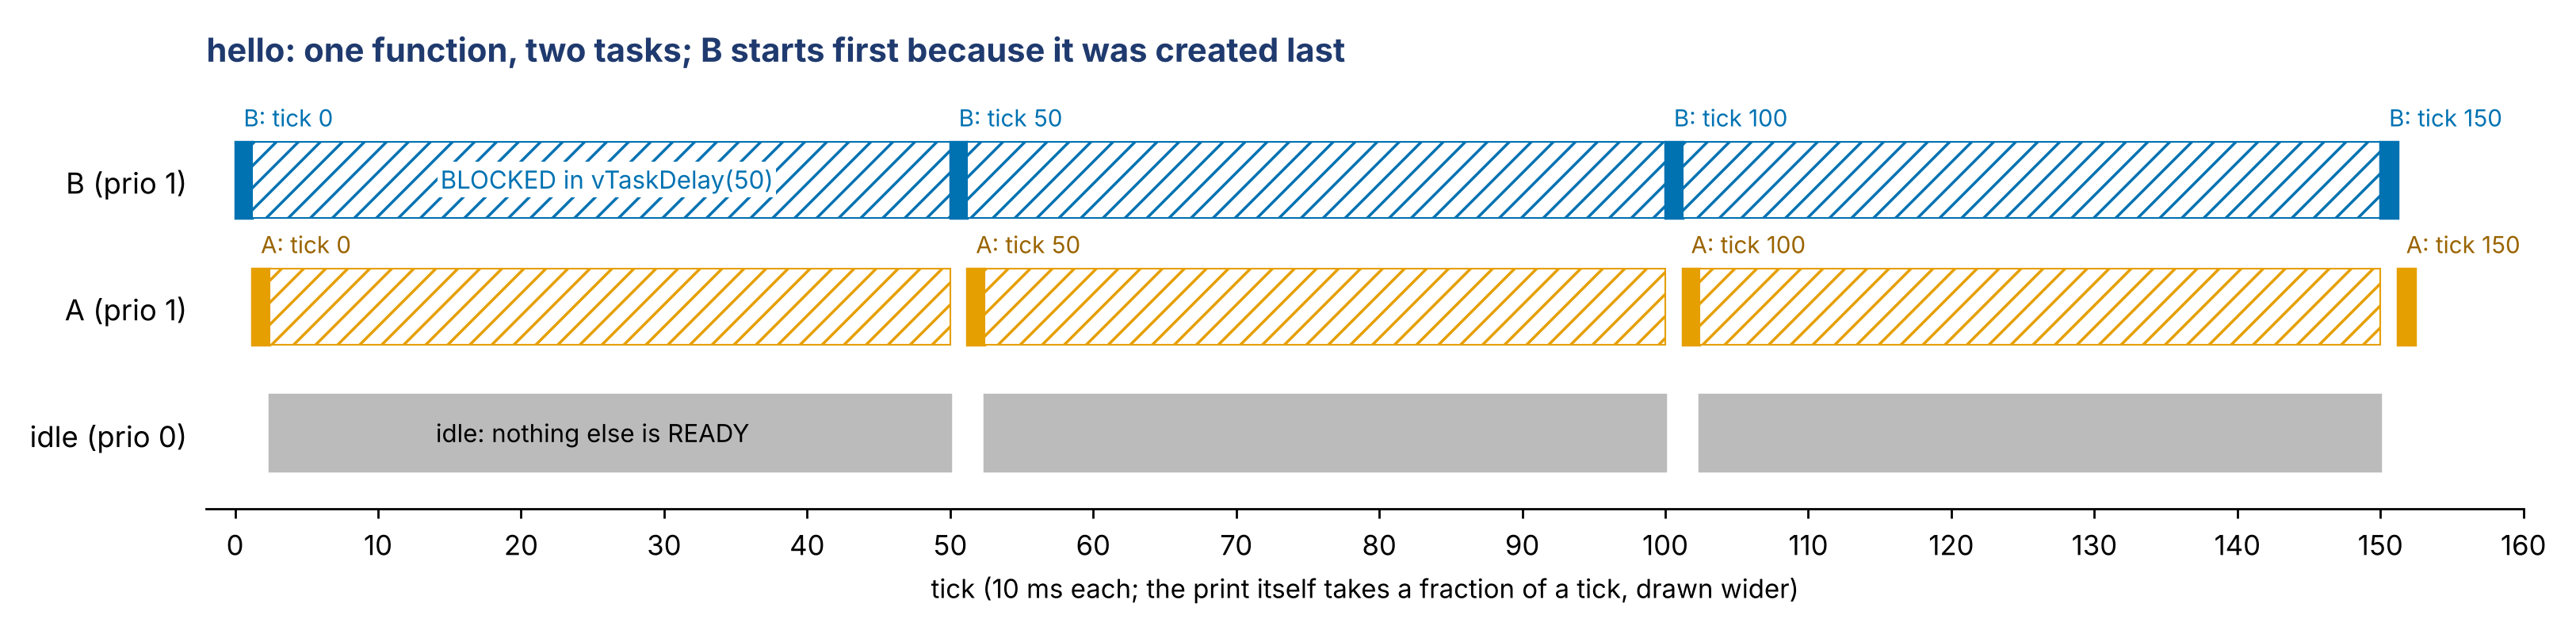
\includegraphics[width=1\textwidth]{contents/images/week-07/hello_timeline.png}
    \caption{The \texttt{hello} run. Every 50 ticks B prints, then A; each one blocks for 50 ticks in \texttt{vTaskDelay}, and the idle task fills the gaps.}
\end{figure}

\subsection{The periodic-task template}
A periodic task must do its job every $T$ ticks. You know the two ways from week 5, \texttt{task\_delay( T )} and \texttt{task\_delay\_until( \&last\_wake, T )}; FreeRTOS has the same pair:
\begin{itemize}
    \item \textbf{\texttt{vTaskDelay( T )}} is \textbf{relative}: sleep $T$ ticks from now, after the work; the period is $T$ + the work time, so the wake-ups \textbf{drift}. Like \texttt{task\_delay} in week 5.
    \item \textbf{\texttt{vTaskDelayUntil( \&last, T )}} is \textbf{absolute}: sleep until tick \texttt{last + T}, then \texttt{last += T}. The work time does not count: the period is exactly $T$ if the work is shorter than $T$, no drift. Like \texttt{task\_delay\_until} in week 5. Set \texttt{last = xTaskGetTickCount()} once, before the loop; its type \texttt{TickType\_t} is the kernel's tick type (32 bits here). \texttt{vTaskDelayUntil} is a macro in \texttt{FreeRTOS/Source/include/task.h} that calls \texttt{xTaskDelayUntil} in \texttt{tasks.c}.
\end{itemize}

\subsection{Try it: write \texttt{periodic}}
Both tasks have priority 1. \texttt{T = 10} ticks, \texttt{ROUNDS = 10}, the table \texttt{work\_ticks[]} (1, 3, 0, 2, 3, 1, 2, 0, 3, 1) and \texttt{busy\_work( n )} are prepared: \texttt{busy\_work} keeps the CPU for $n$ ticks, looping until \texttt{xTaskGetTickCount()} has moved by $n$, without blocking. In \texttt{apps/periodic.c}, replace the whole function \texttt{vTaskP1}, then the whole function \texttt{vTaskP2}, with:
\begin{lstlisting}[language=C, showstringspaces=false, basicstyle=\ttfamily\scriptsize]
static void vTaskP1( void * pvParameters )
{
    ( void ) pvParameters;

    for( int i = 0; i < ROUNDS; i++ )
    {
        console_print( "P1 #%d: woke at tick %lu\n", i,
                       ( unsigned long ) xTaskGetTickCount() );
        busy_work( work_ticks[ i ] ); /* 0 to 3 ticks */
        vTaskDelay( T );               /* T ticks from NOW */
    }
    vTaskSuspend( NULL );              /* done: park it */
}

static void vTaskP2( void * pvParameters )
{
    ( void ) pvParameters;
    TickType_t last = xTaskGetTickCount();   /* first wake */

    for( int i = 0; i < ROUNDS; i++ )
    {
        console_print( "P2 #%d: woke at tick %lu\n", i,
                       ( unsigned long ) xTaskGetTickCount() );
        busy_work( work_ticks[ i ] );
        vTaskDelayUntil( &last, T ); /* until last + T */
    }
    vTaskSuspend( NULL );
}
\end{lstlisting}
The two tasks do the same work; only the delay differs. \texttt{( void ) pvParameters;} tells the compiler that the unused parameter is unused on purpose. After 10 rounds each task parks itself, because a task function must not return. Run \texttt{make APP=periodic run}, and stop QEMU with \texttt{Ctrl-C} when the output stops. What you see (in two columns, to fit):
{\verbatimscriptsize
\begin{verbatim}
periodic: T = 10 ticks, P1 uses vTaskDelay, P2 uses vTaskDelayUntil
P2 #0: woke at tick 0                     P2 #5: woke at tick 50
P1 #0: woke at tick 1                     P2 #6: woke at tick 60
P2 #1: woke at tick 10                    P1 #5: woke at tick 61
P1 #1: woke at tick 12                    P2 #7: woke at tick 70
P2 #2: woke at tick 20                    P1 #6: woke at tick 72
P1 #2: woke at tick 25                    P2 #8: woke at tick 80
P2 #3: woke at tick 30                    P1 #7: woke at tick 84
P1 #3: woke at tick 35                    P2 #9: woke at tick 90
P2 #4: woke at tick 40                    P1 #8: woke at tick 94
P1 #4: woke at tick 47                    P1 #9: woke at tick 107
\end{verbatim}}
P2 wakes at 0, 10, 20, \dots, 90: exactly every $T$. P1 wakes at 1, 12, 25, 35, 47, 61, \dots: after 10 rounds it is 17 ticks late. P2 starts first, for the reason seen in \texttt{hello}: it was created last.

\begin{figure}[H]
    \centering
    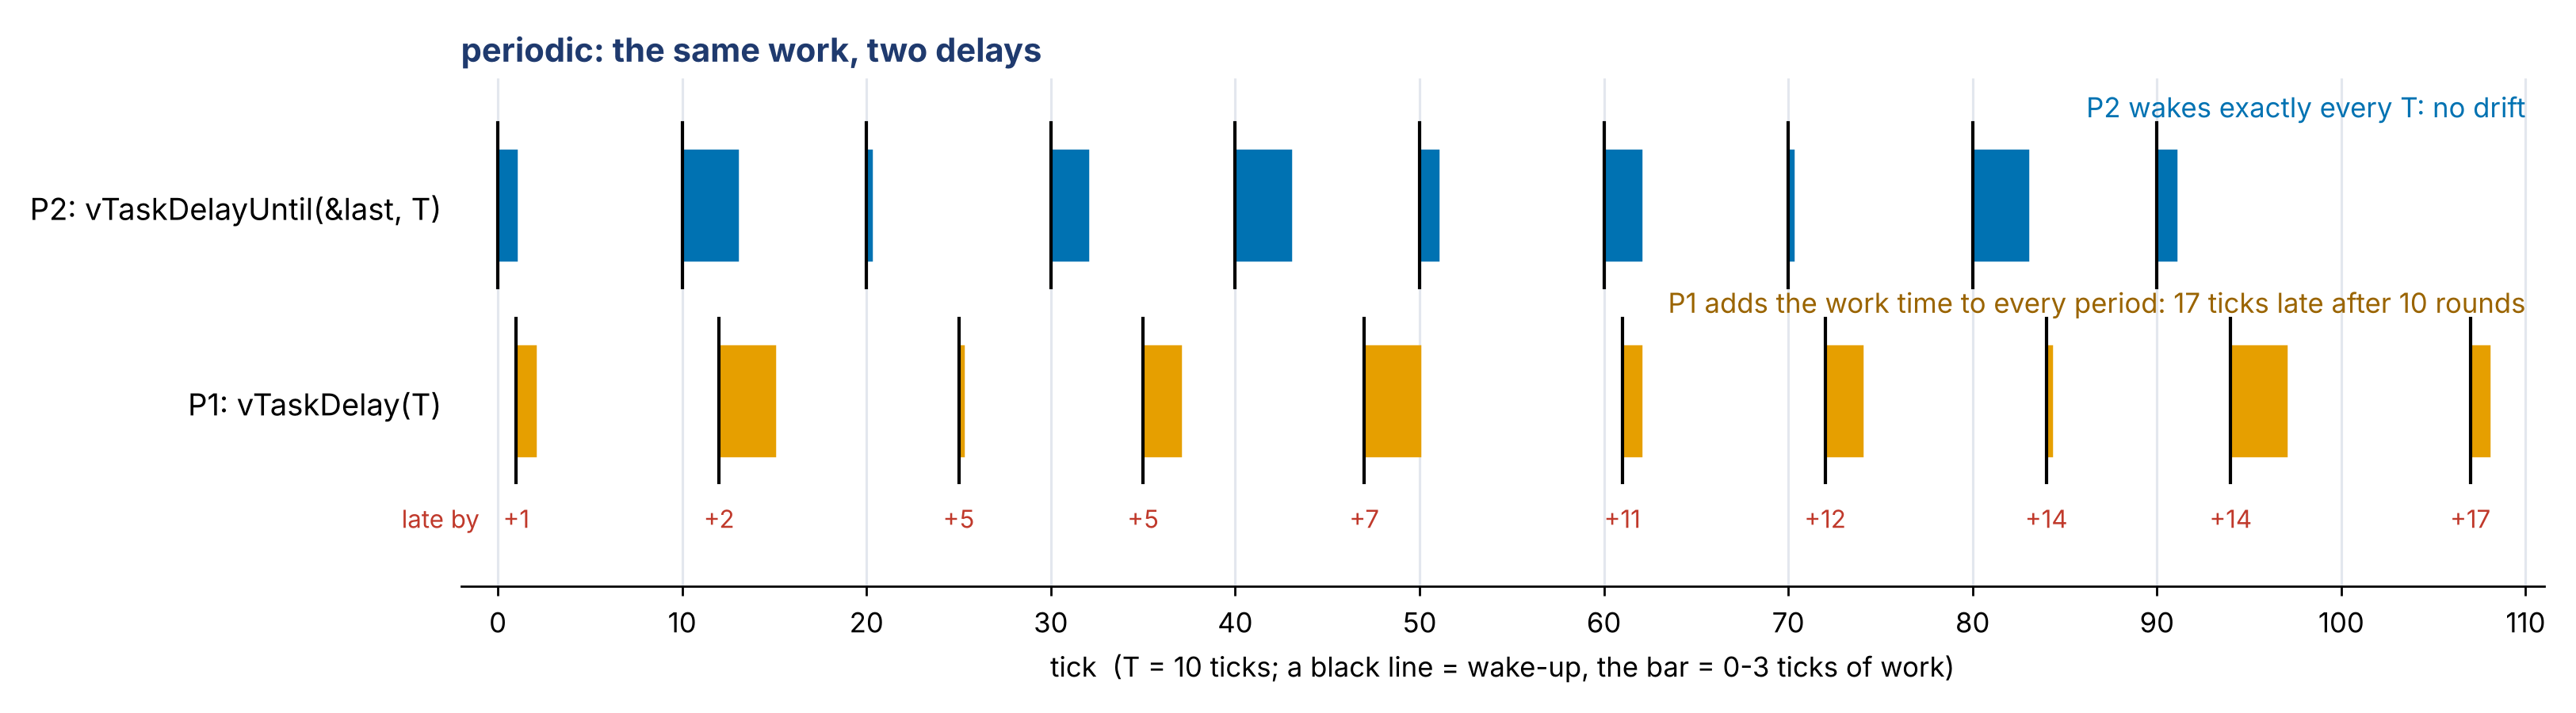
\includegraphics[width=1\textwidth]{contents/images/week-07/periodic_drift.png}
    \caption{The periodic run. Each black line is a wake-up, each bar the work of that round. P2 (\texttt{vTaskDelayUntil}) wakes on every multiple of $T$; P1 (\texttt{vTaskDelay}) adds its work time, and the time it waits for the CPU, to every period, so its lateness grows round after round.}
\end{figure}

\subsection{Observations from the periodic run}
The slide asks three questions: why P1 drifts by the work time of each round, why P1 \#0 wakes at tick 1 and not 0, and why there are 14 ticks between P1 \#4 (47) and P1 \#5 (61) when $T$ + work is 13.
\begin{itemize}
    \item \textbf{The drift}: \texttt{vTaskDelay( T )} counts $T$ ticks from the moment it is called, that is, after the work. So the next wake is at (this wake + work + $T$). Round 1: P1 woke at 12, worked 3 ticks until 15, slept 10 $\to$ woke at 25. The work time is added to every period.
    \item \textbf{P2 does not drift}: \texttt{vTaskDelayUntil} counts from \texttt{last}, the planned wake tick, not from the call. The work happens inside the period: round 1 woke at 10, worked until 13, slept until 20.
    \item \textbf{P1 \#0 at tick 1}: both tasks are READY at tick 0, with the same priority. P2 runs first and does 1 tick of work; at tick 1 the time slice gives the CPU to P1.
    \item \textbf{14 ticks instead of 13}: P1 worked from 47 to 50 (3 ticks), but at tick 50 P2 woke up and, with time slicing, took the CPU for its 1 tick of work. P1 could call \texttt{vTaskDelay} only at tick 51, so it woke at 61. Waiting for the CPU adds to the drift too.
    \item The template for a periodic task is therefore P2's: \texttt{last = xTaskGetTickCount()} once, then a loop of work and \texttt{vTaskDelayUntil( \&last, T )}.
\end{itemize}

\subsection{Priorities and preemption}
FreeRTOS, as configured here, uses \textbf{preemptive fixed-priority} scheduling: you choose each task's priority when you create it, and the kernel never changes it.
\begin{itemize}
    \item At every moment the running task is a READY task of the highest priority (new idea 1). If a more urgent task becomes READY, at a tick or because another task woke it, it takes the CPU at once: the running task is preempted and stays READY.
    \item Tasks of the same priority take turns, one tick each (time slicing).
    \item A task of lower priority runs only while every more urgent task is blocked. If a more urgent task never blocks, the lower ones never run: they \textbf{starve}, as in the exercises of week 5.
    \item There is no aging here: it is your job, when you write a task, to make it \textbf{block} (for example with \texttt{vTaskDelay}) when it has nothing to do.
\end{itemize}
\begin{figure}[H]
    \centering
    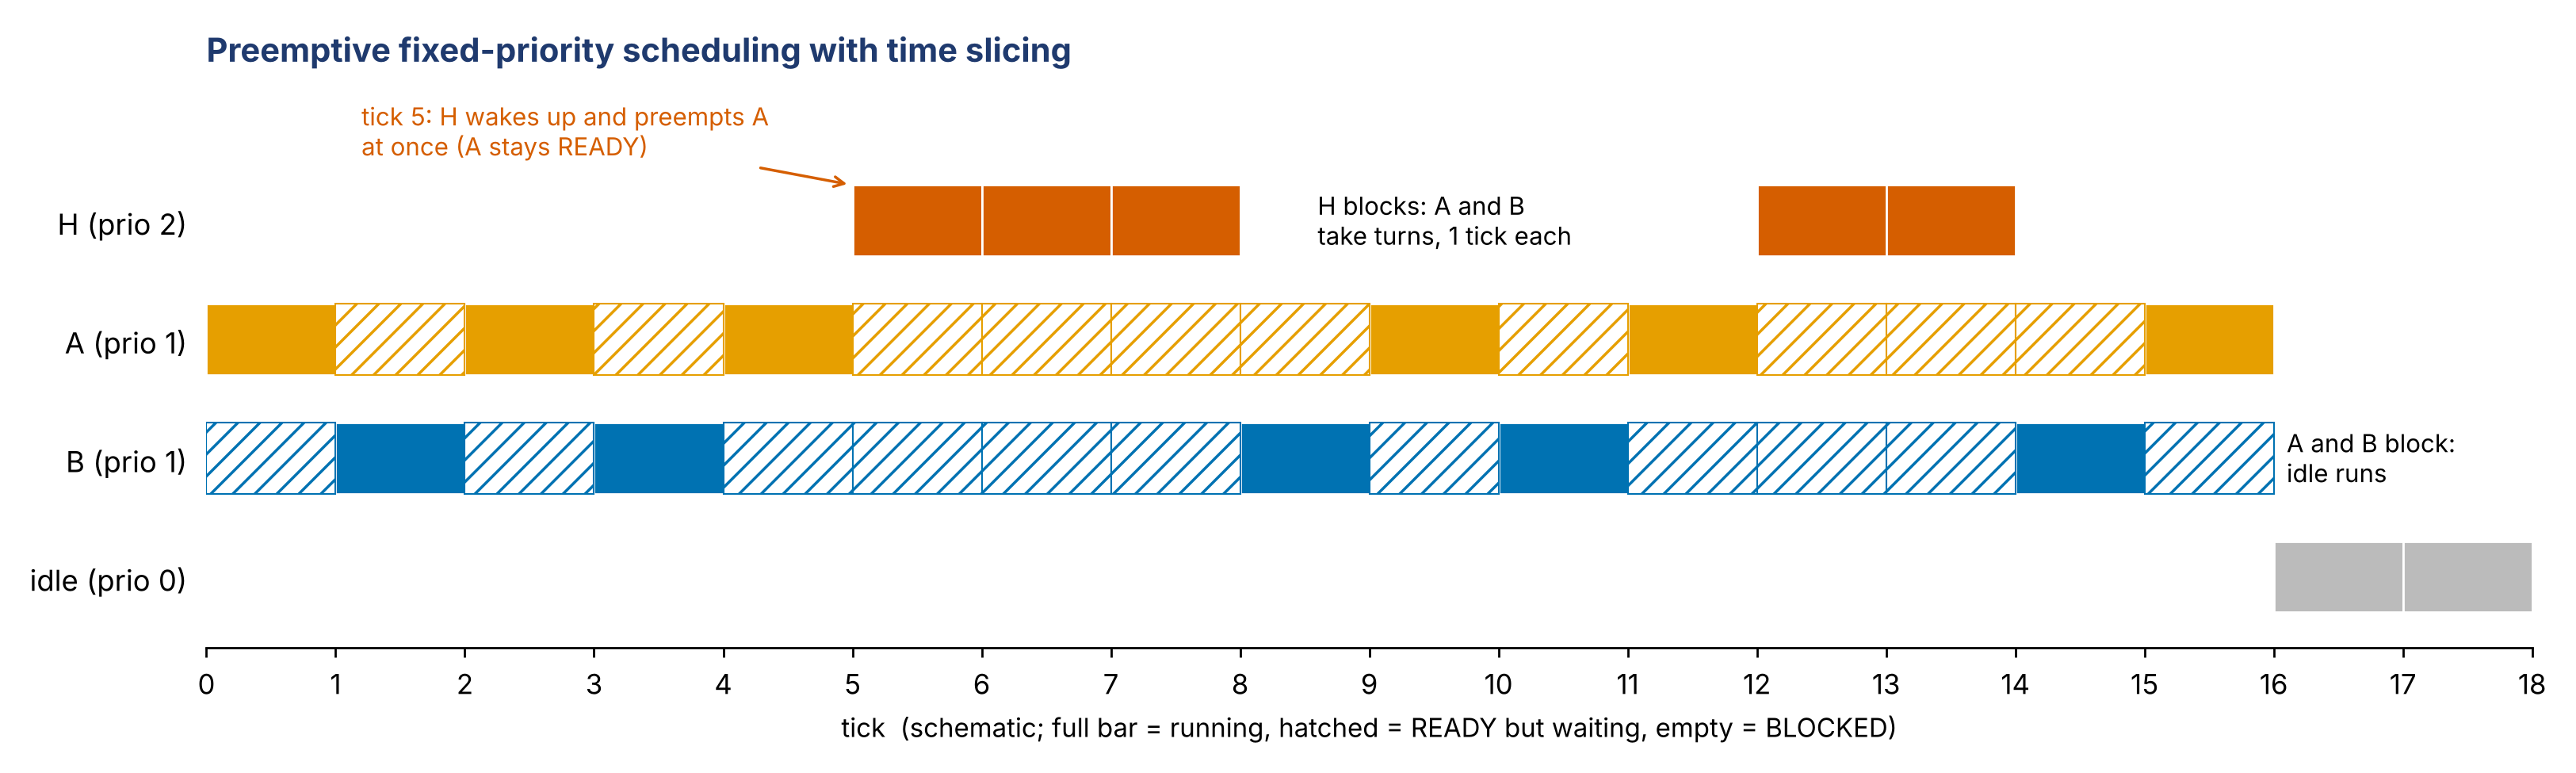
\includegraphics[width=1\textwidth]{contents/images/week-07/preemption.png}
    \caption{The rules at work (schematic). A and B, same priority, take turns every tick; when H becomes READY it takes the CPU at once, and the preempted task stays READY; when H blocks, A and B take turns again; the idle task runs only when everybody else is blocked.}
\end{figure}

\subsection{Try it: write \texttt{starve}, then the fix}
\texttt{WORK\_STEPS} (10\,000\,000 loop steps, a few ticks of busy work) is prepared. \texttt{main()} creates High with priority 2 and Low with priority 1. In \texttt{apps/starve.c}, replace the whole function \texttt{vTaskHigh}, then the whole function \texttt{vTaskLow}, with:
\begin{lstlisting}[language=C, showstringspaces=false, basicstyle=\ttfamily\scriptsize]
static void vTaskHigh( void * pvParameters )
{
    ( void ) pvParameters;
    unsigned long round = 0;

    for( ;; )
    {
        for( volatile unsigned long i = 0; i < WORK_STEPS; i++ )
        {
        }                         /* busy work, no blocking */
        console_print( "High: round %lu (tick %lu)\n", round++,
                       ( unsigned long ) xTaskGetTickCount() );
#ifdef DEMO_FIXED
        vTaskDelay( 1 );          /* the fix: block 1 tick */
#endif
    }
}

static void vTaskLow( void * pvParameters )
{
    ( void ) pvParameters;

    for( ;; )
    {
        console_print( "Low ran (tick %lu)\n",
                       ( unsigned long ) xTaskGetTickCount() );
        vTaskDelay( pdMS_TO_TICKS( 100 ) ); /* 10 ticks */
    }
}
\end{lstlisting}
\texttt{volatile} stops the compiler from removing the empty loop: without it, the compiler could see that the loop computes nothing and drop it. The fix is written already, but it is compiled only with \texttt{DEMO=fixed}, which defines \texttt{DEMO\_FIXED}. Run \texttt{make APP=starve run}, look, stop with \texttt{Ctrl-C}; then run \texttt{make APP=starve DEMO=fixed run}. Your tick numbers may differ a little: the busy loop counts steps, so its length depends on the speed of your computer.
{\verbatimscriptsize
\begin{verbatim}
starve: High (priority 2) never blocks         starve: ... except for vTaskDelay(1) ...
High: round 0 (tick 2)                         High: round 0 (tick 2)
High: round 1 (tick 5)                         Low ran (tick 2)
High: round 2 (tick 8)                         High: round 1 (tick 6)
High: round 3 (tick 11)                        High: round 2 (tick 10)
High: round 4 (tick 14)                        High: round 3 (tick 14)
High: round 5 (tick 17)                        Low ran (tick 14)
... (no "Low ran", ever)                       High: round 4 (tick 18)
                                               High: round 5 (tick 21)
                                               High: round 6 (tick 24)
                                               Low ran (tick 24)
                                               ...
\end{verbatim}}
Left: Low is READY from tick 0, but High is always READY too, and more urgent: Low \textbf{starves}. Right (banner cut to fit): Low runs again.
\begin{figure}[H]
    \centering
    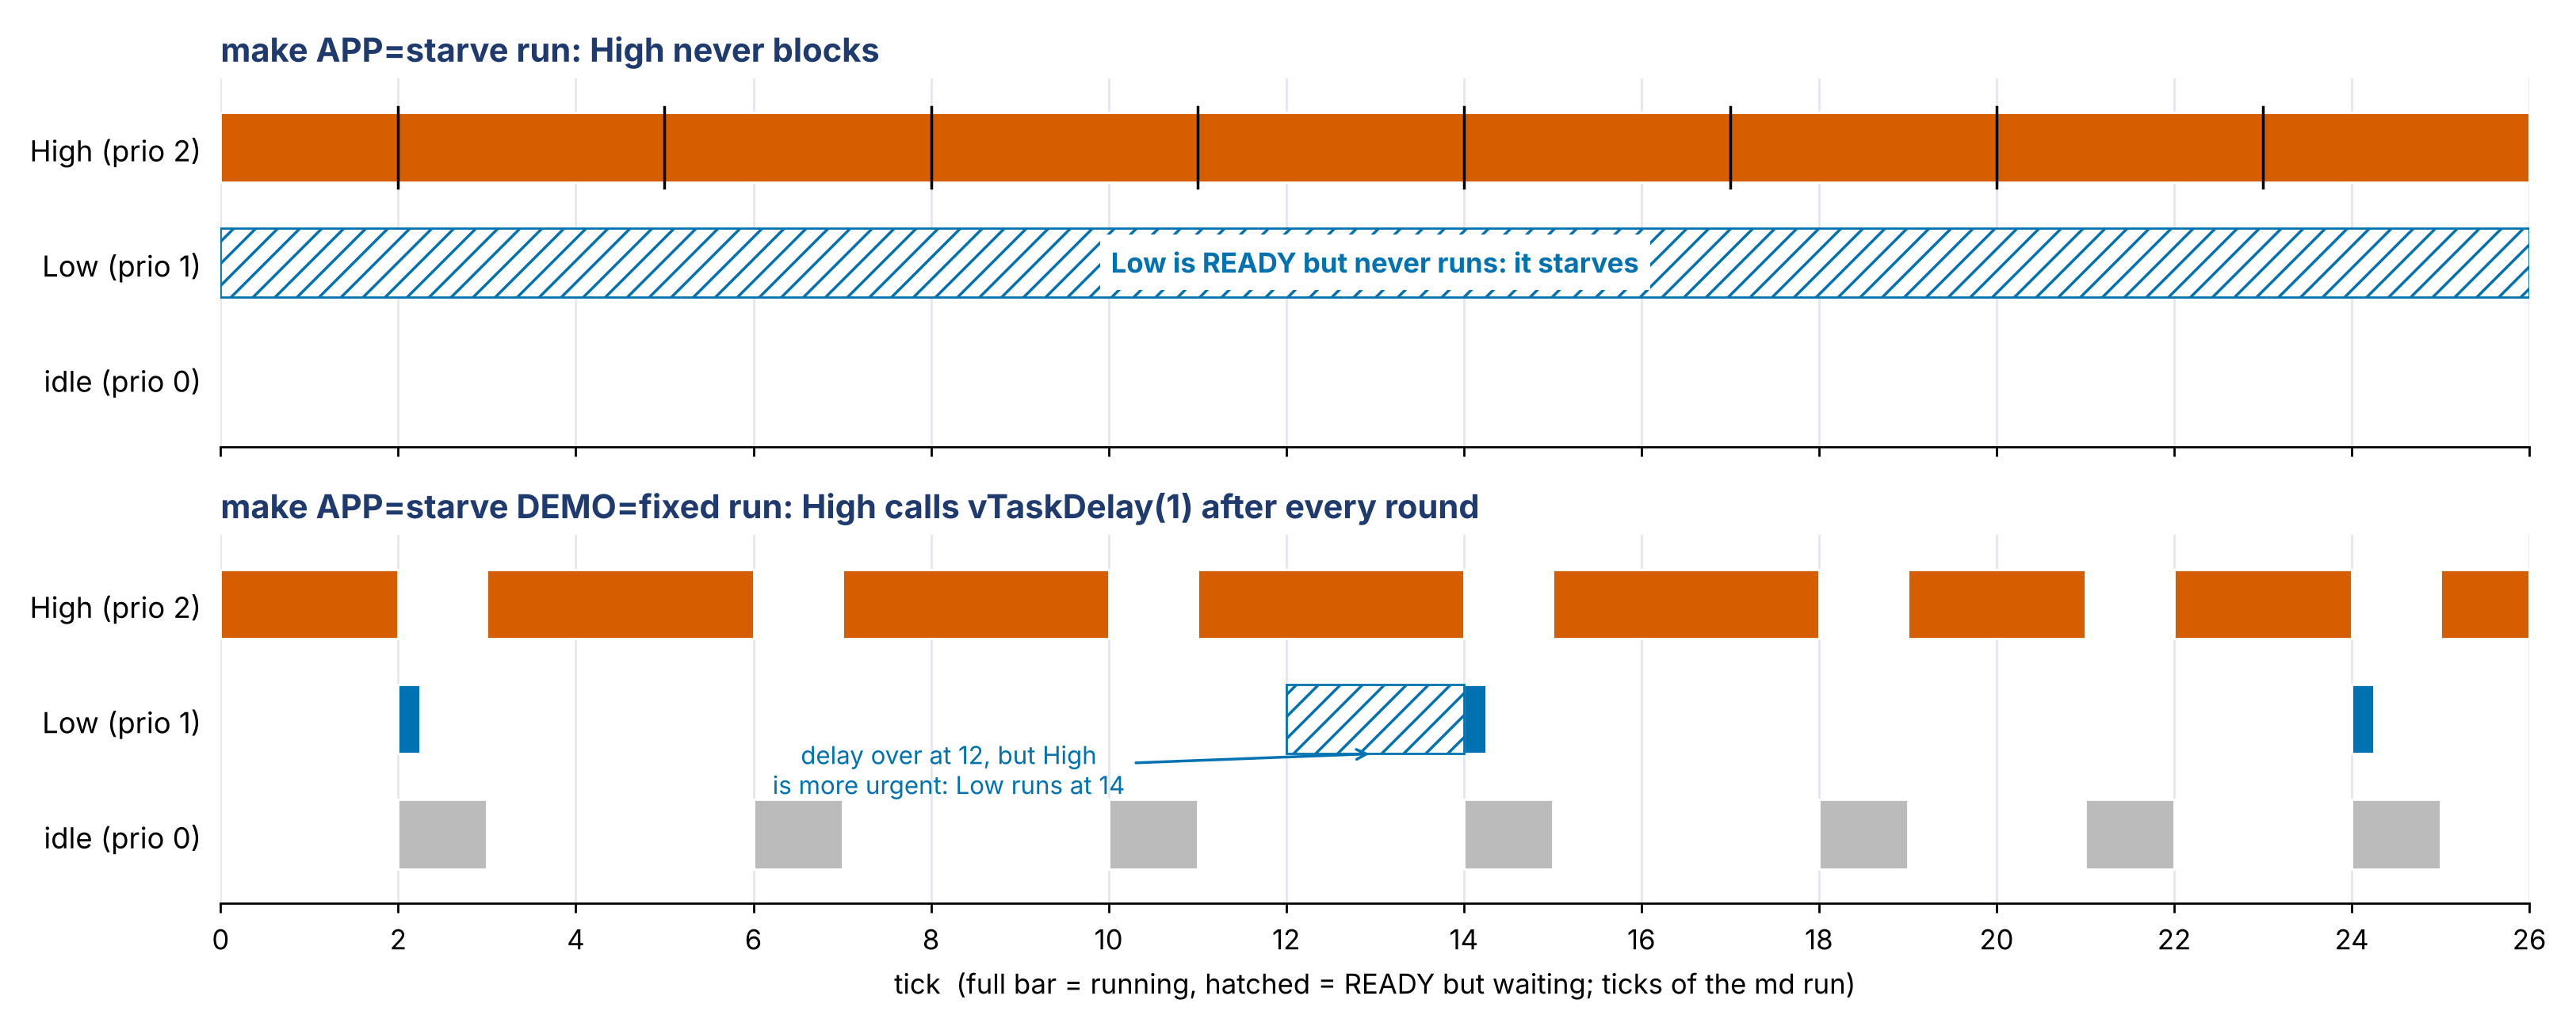
\includegraphics[width=1\textwidth]{contents/images/week-07/starve_timeline.png}
    \caption{The two \texttt{starve} runs on a timeline. Top: High never blocks, Low never runs. Bottom: High blocks one tick after every round; Low runs at ticks 2, 14 and 24, and the idle task fills the other gaps.}
\end{figure}

\subsection{Observations from the starvation run}
The slide asks three questions: why a delay of one tick is enough, why Low does not run after every round of High, and why Low, which printed at tick 2 and asked to sleep 10 ticks, prints again at 14 and not 12.
\begin{itemize}
    \item \textbf{One tick is plenty}: when High calls \texttt{vTaskDelay( 1 )}, it leaves the ready list until the next tick. The most urgent READY task is now Low, so Low runs at once. Low needs only a few microseconds: it prints one line and blocks itself for 10 ticks.
    \item \textbf{Low runs only every 10 ticks}: after printing, Low is in the delayed list until its 100\,ms are over. In the other gaps of High, nobody but the idle task is READY, so the idle task fills them.
    \item \textbf{14, not 12}: Low printed at tick 2 and asked to sleep 10 ticks, so its delay ends at tick 12, while High is in the middle of a round. Low becomes READY, but High is more urgent, so Low waits until High's next \texttt{vTaskDelay( 1 )}, at tick 14. A lower-priority task only gets the time the more urgent tasks leave free.
    \item \textbf{The lesson}: a task with a high priority must \textbf{block} when it has nothing urgent to do; a delay, even a short one, gives the CPU to the tasks below it.
\end{itemize}

\subsection{Look inside with gdb: \texttt{pxCurrentTCB} (optional)}
This optional session shows the scheduler's data while \texttt{hello} runs: who is current, which ready list holds which tasks, and the delayed list. Unlike the scratch OS, this port has \textbf{no MPU} and every task is privileged, so gdb can read every kernel variable at every stop, not only in the handlers.

\paragraph{Setting up.} In \texttt{freertos-labs/week-07/solution/} (or in your base, once \texttt{hello.c} is written) run \texttt{make APP=hello debug}: QEMU starts frozen and waits for gdb on port 1234. In a second terminal, in the same folder, run \texttt{arm-none-eabi-gdb build/hello.elf} (on Linux: \texttt{gdb-multiarch}).

\begin{figure}[H]
    \centering
    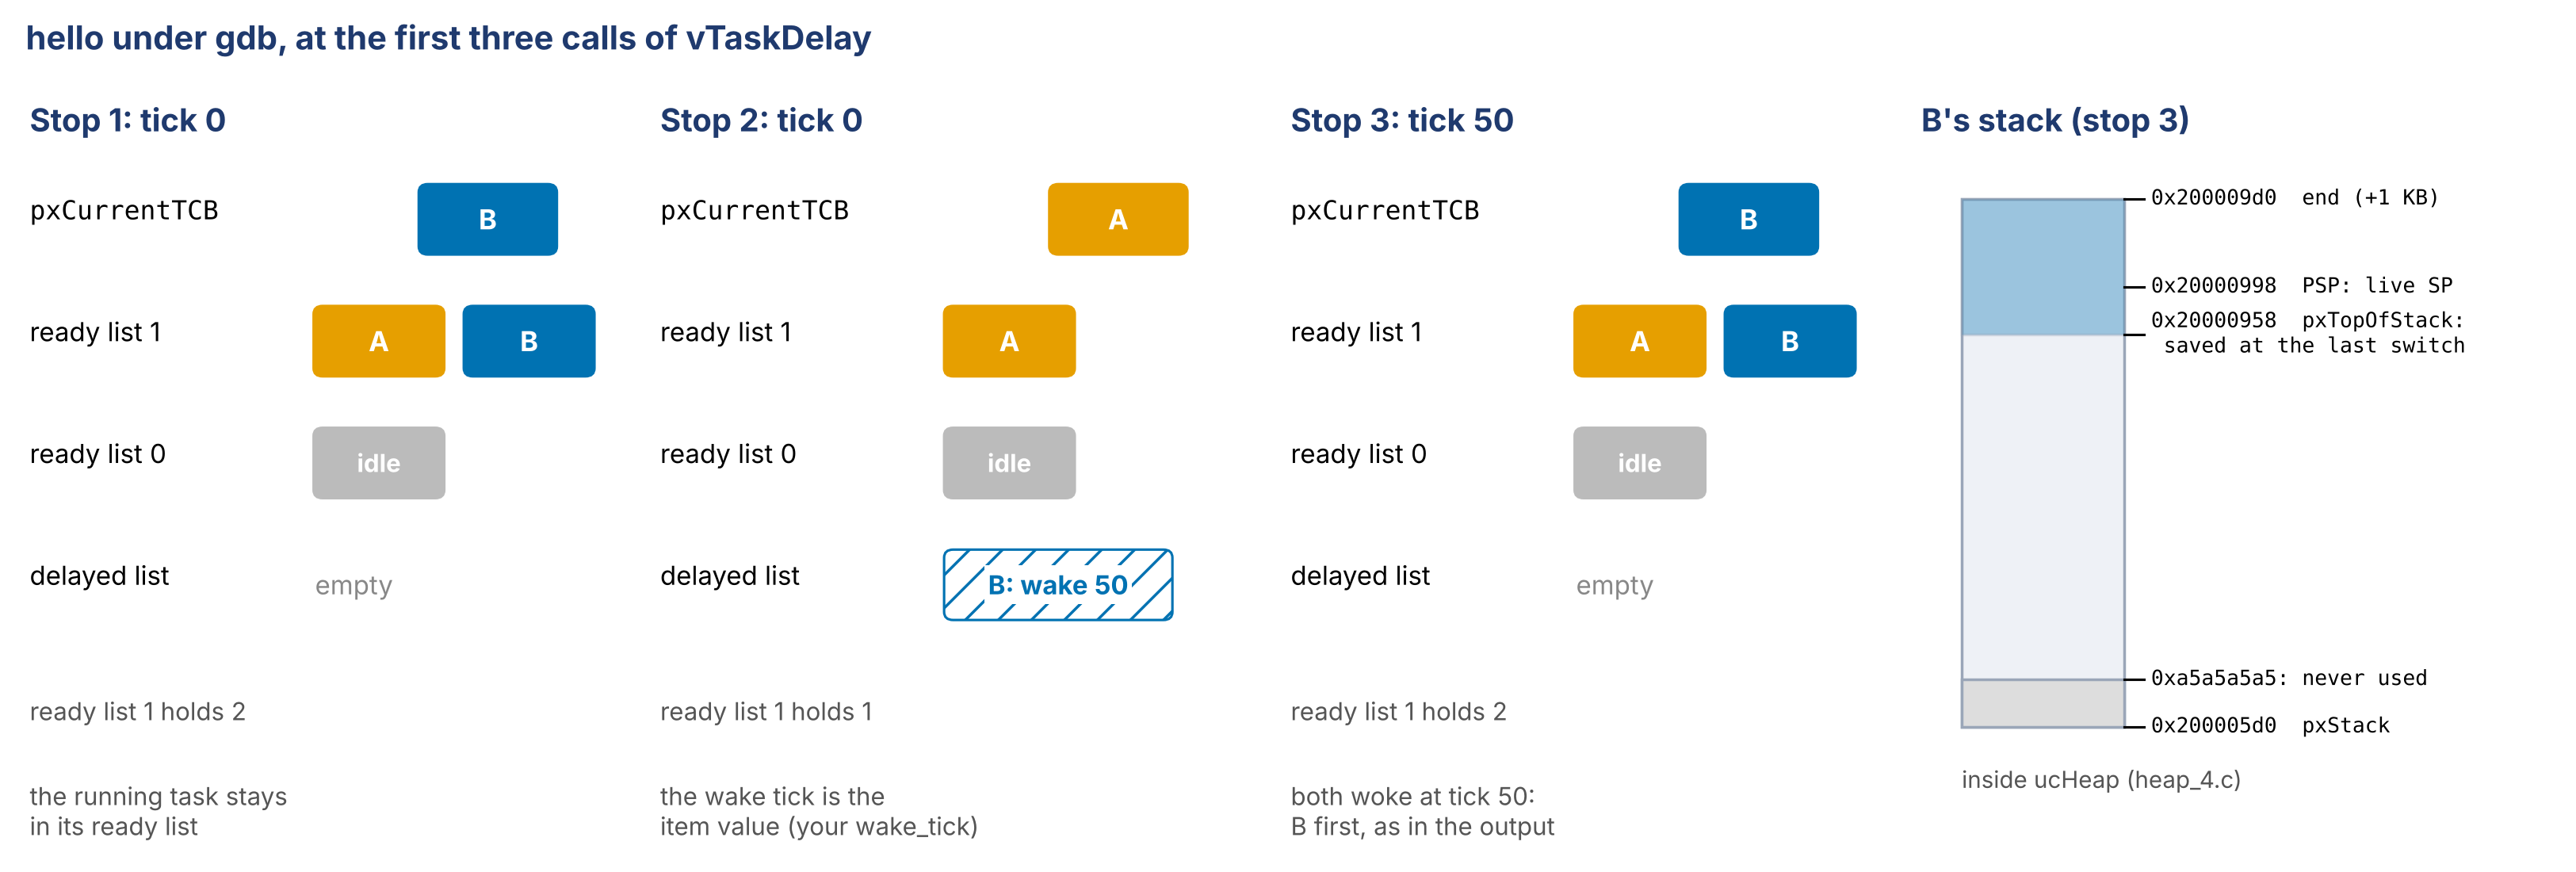
\includegraphics[width=1\textwidth]{contents/images/week-07/freertos_lists_gdb.png}
    \caption{What gdb shows at the three stops: the current task, the ready lists, the delayed list, and B's stack inside the heap.}
\end{figure}

\paragraph{Stop 1: the first \texttt{vTaskDelay}.} The source lines that gdb prints at each stop are left out:
{\verbatimscriptsize
\begin{verbatim}
(gdb) target remote :1234
(gdb) break vTaskDelay
(gdb) continue
(gdb) p xTickCount
(gdb) p pxCurrentTCB->pcTaskName
(gdb) p pxCurrentTCB->uxPriority
(gdb) p pxReadyTasksLists[1].uxNumberOfItems
(gdb) p pxReadyTasksLists[0].uxNumberOfItems
(gdb) p uxTopReadyPriority

Breakpoint 1 at 0x818: file ../../FreeRTOS/Source/tasks.c.
Breakpoint 1, vTaskDelay (xTicksToDelay=50) at ../../FreeRTOS/Source/tasks.c
$1 = 0
$2 = "B\000\000\000\000\000\000\000\000"
$3 = 1
$4 = 2
$5 = 1
$6 = 1
\end{verbatim}}
The first to call \texttt{vTaskDelay} is \textbf{B}, at tick 0, with 50 ticks: the ``B prints first'' of \texttt{hello}, from inside. Ready list 1 holds \textbf{2} tasks, A and B: the \textbf{running task stays in its ready list}; list 0 holds the idle task; \texttt{uxTopReadyPriority} is 1.

\paragraph{Stop 2: the next call.}
{\verbatimscriptsize
\begin{verbatim}
(gdb) continue
(gdb) p xTickCount
(gdb) p pxCurrentTCB->pcTaskName
(gdb) p pxReadyTasksLists[1].uxNumberOfItems
(gdb) p pxDelayedTaskList->uxNumberOfItems
(gdb) p pxDelayedTaskList->xListEnd.pxNext->xItemValue

Breakpoint 1, vTaskDelay (xTicksToDelay=50) at ../../FreeRTOS/Source/tasks.c
$7 = 0
$8 = "A\000\000\000\000\000\000\000\000"
$9 = 1
$10 = 1
$11 = 50
\end{verbatim}}
Still tick 0, now \textbf{A} is current: B moved from ready list 1 to the delayed list. \texttt{xListEnd} is the end marker of every FreeRTOS list, and its \texttt{pxNext} is the first item: its value, \textbf{50}, is B's wake tick, where your \texttt{wake\_tick} went.

\paragraph{Stop 3: tick 50.}
{\verbatimscriptsize
\begin{verbatim}
(gdb) continue
(gdb) p xTickCount
(gdb) p pxCurrentTCB->pcTaskName
(gdb) p pxCurrentTCB->pxStack
(gdb) p pxCurrentTCB->pxTopOfStack
(gdb) p/x $psp
(gdb) x/2wx pxCurrentTCB->pxStack
(gdb) p pxDelayedTaskList->uxNumberOfItems

Breakpoint 1, vTaskDelay (xTicksToDelay=50) at ../../FreeRTOS/Source/tasks.c
$12 = 50
$13 = "B\000\000\000\000\000\000\000\000"
$14 = (StackType_t *) 0x200005d0 <ucHeap+1144>
$15 = (volatile StackType_t *) 0x20000958 <ucHeap+2048>
$16 = 0x20000998
0x200005d0 <ucHeap+1144>:  0xa5a5a5a5  0xa5a5a5a5
$17 = 0
\end{verbatim}}
Tick 50: \textbf{B} again, then A. B's stack (\texttt{pxStack = 0x200005d0}, 256 words, up to \texttt{0x200009d0}) is inside \texttt{ucHeap}, the 64\,KB array of \texttt{heap\_4.c}: it came from the \textbf{heap}. \texttt{pxTopOfStack} (\texttt{0x20000958}) is \textbf{not} the live SP: it was saved at B's last switch out; while B runs, the live SP is PSP (\texttt{0x20000998}). The lowest words still hold \texttt{0xa5a5a5a5}: B never used that deep. The delayed list is empty: both tasks woke at tick 50.
The run is deterministic, so you should see the same values; only the addresses may differ slightly with another compiler version. Quit gdb with \texttt{quit} (answer \texttt{y}), and QEMU with \texttt{Ctrl-C} in its terminal.

\section{Unit 3: summary}
\begin{itemize}
    \item FreeRTOS runs on the \textbf{same board and QEMU}. The kernel is given and never edited; you write tasks in \texttt{apps/}, with the board support in \texttt{bsp/} and the settings in \texttt{FreeRTOSConfig.h}.
    \item \textbf{Project layout and configuration}: \texttt{apps/}, \texttt{bsp/}, the kernel compiled from \texttt{FreeRTOS/Source} and never edited (extend it with hooks); \texttt{FreeRTOSConfig.h} (10\,ms tick, preemption, time slicing, 5 priorities, 64\,KB heap, checks).
    \item \textbf{Same mechanisms as your kernel}: \texttt{TCB\_t} with \texttt{pxTopOfStack} first, \texttt{pxPortInitialiseStack} builds the fake frame (with \texttt{r0 = pvParameters}), PendSV saves/chooses/restores (\texttt{xPortPendSVHandler}), SysTick counts and asks (\texttt{xTaskIncrementTick}), the first task starts with an SVC and an exception return, and an idle task runs when nobody else can. But every task is privileged, with no MPU.
    \item \textbf{New ideas}: one ready list per priority (the highest non-empty list runs, round robin inside it, the tick is the time slice); critical sections and the scheduler's decision with \textbf{BASEPRI}, which leaves the most urgent interrupts unmasked, and a nesting counter.
    \item \textbf{The task function}: \texttt{void vTask( void * pvParameters )}, set-up then \texttt{for( ;; )}, never returns; park a finished task with \texttt{vTaskSuspend( NULL )}.
    \item \texttt{xTaskCreate( function, name, stack in words, parameter, priority, handle )}: TCB and stack from the heap, at any time. \texttt{vTaskStartScheduler()}: creates the idle task, starts the first task, never returns.
    \item \textbf{Priorities and preemption}: higher $=$ more urgent; the highest READY task runs, equal ones take turns, a task that never blocks starves the ones below. The idle task: priority 0, created for you, runs when nothing else is READY.
    \item \texttt{vTaskDelay( T )} vs \texttt{vTaskDelayUntil( \&last, T )}: relative, drifts by the work time; absolute, no drift. The periodic-task template: \texttt{last = xTaskGetTickCount();} then \texttt{for( ;; ) \{ work; vTaskDelayUntil( \&last, T ); \}}.
    \item \texttt{console\_print( fmt, ... )}: formats the whole line, then sends it inside a critical section.
\end{itemize}

\section{Week 7: where to find the code}
\paragraph{Scratch OS.} \texttt{scratch-os/week-07/} holds \texttt{base/} and \texttt{solution/}, each with its own \texttt{Makefile}. The base is the week 5 kernel with the shared region, the two-phase program, the demo builds and three empty lock functions. The files that changed this week, compared with week 5 (paths relative to \texttt{scratch-os/week-07/solution/}):
\begin{itemize}
    \item \texttt{lib/spinlock.s} and \texttt{lib/spinlock.h}: the spinlock, the part you write;
    \item \texttt{src/shared.h} and \texttt{src/shared.c}: the \texttt{SHARED} marker and the shared variables;
    \item \texttt{scripts/mps2\_m3.ld}: the \texttt{.shared} section;
    \item \texttt{kernel/mpu.c}: region 2 in \texttt{mpu\_init};
    \item \texttt{src/tasks.h}, \texttt{src/task\_a.c} and \texttt{src/task\_b.c}: the two-phase program, \texttt{plus\_one}, the \texttt{LOCK}/\texttt{UNLOCK} and \texttt{PRINT\_BEGIN}/\texttt{PRINT\_END} macros;
    \item \texttt{Makefile}: the \texttt{race}, \texttt{counter}, \texttt{cpsid} and \texttt{spin} demos.
\end{itemize}

\paragraph{FreeRTOS.} \texttt{freertos-labs/week-07/} holds \texttt{base/} and \texttt{solution/}; the kernel is in \texttt{freertos-labs/FreeRTOS/Source/}. The base has everything except the bodies of the task functions in \texttt{apps/hello.c}, \texttt{apps/periodic.c} and \texttt{apps/starve.c}. In the solution (paths relative to \texttt{freertos-labs/week-07/solution/}):
\begin{itemize}
    \item \texttt{Makefile} and \texttt{FreeRTOSConfig.h}: the build and the kernel settings;
    \item \texttt{bsp/startup.c}, \texttt{bsp/mps2\_m3.ld}, \texttt{bsp/uart.c}, \texttt{bsp/syscalls.c}, \texttt{bsp/console.c} and \texttt{bsp/hooks.c}: the board support;
    \item \texttt{apps/hello.c}, \texttt{apps/periodic.c} and \texttt{apps/starve.c}: the three programs.
\end{itemize}
Every file in both solution folders is commented line by line. If these notes and the code ever disagree, the code is the reference.

\section{A prova di coglione}
Fino alla settimana scorsa i task dello scratch-OS erano \emph{indipendenti}: ognuno nella sua partizione, senza niente in comune, e anche la teoria dello scheduling assumeva task indipendenti. Questa settimana rompe questa regola: due task che condividono qualcosa (una variabile, ma anche solo la UART) si danneggiano a vicenda, a meno che non si mettano d'accordo su chi passa per primo. Il percorso è diviso in tre unità.

\begin{itemize}
    \item \textbf{Unità 1: le idee (solo teoria).} Due demo mostrano il problema: righe di testo mescolate e un contatore che perde aggiornamenti. Poi le parole per descriverlo (risorsa condivisa, race condition, interleaving, sezione critica), i tre requisiti di ogni soluzione e gli strumenti: mascherare gli interrupt, lo spinlock costruito su un'istruzione atomica, il semaforo e il mutex. Gli esercizi sugli interleaving e sulle tracce dei semafori sono di tipo d'esame.
    \item \textbf{Unità 2: uno spinlock nello scratch-OS.} Si scrive un solo file, \texttt{lib/spinlock.s}, in assembly: prima un lock che aspetta girando a vuoto (\emph{busy waiting}), poi uno che cede la CPU mentre aspetta (\emph{spin-then-yield}). Il trace dello scheduler mostra quanto costa ciascuno. È l'ultima implementazione di kernel del corso.
    \item \textbf{Unità 3: FreeRTOS.} Un kernel vero, usato nell'industria, sulla stessa scheda e nello stesso QEMU. Si scopre che è costruito sugli stessi meccanismi dello scratch-OS (TCB, frame finto, PendSV, SysTick, idle), con due idee nuove: una lista READY per ogni priorità e le sezioni critiche con BASEPRI. Poi si scrivono i primi tre programmi: \texttt{hello}, \texttt{periodic} e \texttt{starve}.
\end{itemize}

In breve: prima \emph{perché} i task condivisi vanno sincronizzati, poi \emph{come} si costruisce davvero un lock a basso livello, infine \emph{dove} si va da qui in avanti: un kernel reale, che non si modifica più, ma si usa.

\subsection{Unità 1}

\paragraph*{L'idea.} Su una CPU sola i task si alternano, e il tick può togliere la CPU a un task \textbf{tra due istruzioni qualsiasi}. Se due task lavorano sullo stesso dato e uno viene interrotto a metà di un'operazione, l'altro può vedere o scrivere un valore ``a metà''. Bisogna individuare il pezzo di codice pericoloso (la \textbf{sezione critica}) e fare in modo che un solo task alla volta ci entri.

\subsubsection*{1. Due demo, un solo problema}
\paragraph*{\texttt{DEMO=race}: righe mescolate.} A e B stampano 3000 righe di 100 lettere ciascuno sulla stessa UART. Quasi tutte le righe sono giuste, ma alcune (13 su 6000 in una run, un numero diverso a ogni run) sono spezzate, e il taglio cade \textbf{sempre dopo circa 64 lettere}. Il motivo:
\begin{itemize}
    \item \texttt{printf} formatta in un buffer di \textbf{64 byte}: una riga da 101 byte (100 lettere + \texttt{\textbackslash n}) esce in \textbf{due} chiamate a \texttt{sys\_write}, 64 byte e poi 37;
    \item ogni \texttt{sys\_write} è atomica (una system call arriva sempre in fondo), ma il tick può cadere \textbf{tra} le due chiamate: allora B stampa i suoi 64 byte in mezzo alla riga di A;
    \item \textbf{la chiamata è atomica, la riga no.} La risorsa condivisa qui è la UART, ed è nascosta in una funzione di libreria: le dipendenze non si vedono sempre nel codice dell'applicazione.
\end{itemize}

\paragraph*{\texttt{DEMO=counter}: aggiornamenti persi.} A e B incrementano 1\,000\,000 di volte ciascuno lo stesso \texttt{shared\_counter}. Ci si aspetta 2\,000\,000, si ottiene meno (1\,314\,814, 1\,099\,261, \dots), mai lo stesso valore due volte, e \textbf{nessun errore}: il programma ``funziona'' e il risultato è semplicemente sbagliato. Il motivo è che \texttt{x = x + 1} non è un passo solo, ma tre istruzioni:
\begin{center}
\texttt{ldr r0, [r1]} (load) $\quad\to\quad$ \texttt{adds r0, \#1} (add, nel registro) $\quad\to\quad$ \texttt{str r0, [r1]} (store)
\end{center}
Il registro è \textbf{privato} (lo switch lo salva sullo stack del task), la variabile in memoria è \textbf{condivisa}. Se uno switch cade tra il load e lo store di A e B intanto aggiorna il contatore, quando A scrive cancella il lavoro di B: è il \textbf{lost update}.

\begin{figure}[H]
    \centering
    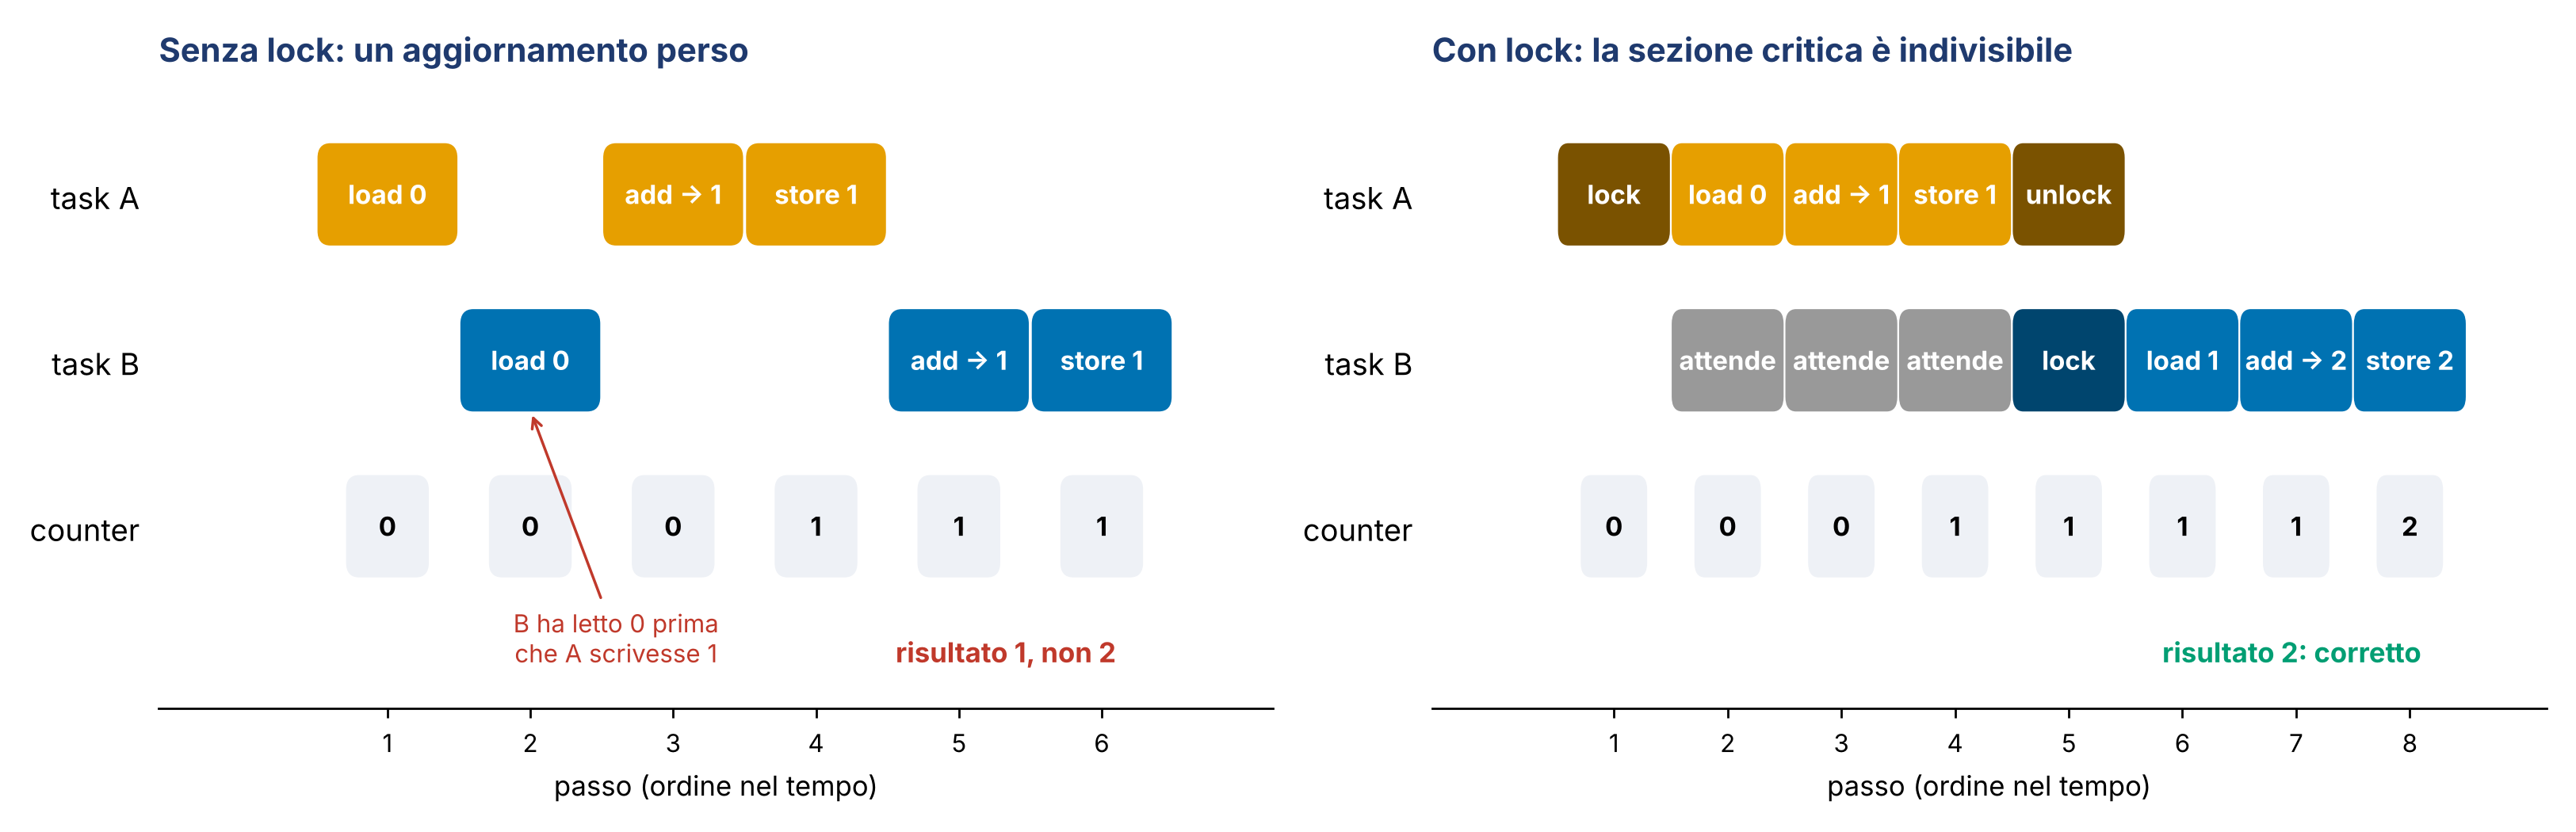
\includegraphics[width=1\textwidth]{contents/images/week-07/it_lost_update.png}
    \caption{A sinistra: A e B caricano entrambi 0 prima che uno dei due abbia scritto, quindi tutti e due scrivono 1 e un incremento va perso. A destra: con un lock attorno a load-add-store, B aspetta alla porta, legge l'1 scritto da A e il risultato è 2.}
\end{figure}

\paragraph*{Perché la demo ha bisogno di \texttt{plus\_one}.} Con il semplice \texttt{x = x + 1} sotto QEMU non si perdeva \emph{nessun} aggiornamento. QEMU traduce blocchi di istruzioni (un blocco finisce a un salto) e controlla gli interrupt \textbf{solo tra un blocco e l'altro}: load, add e store stanno nello stesso blocco, quindi il tick non cade mai in mezzo. Un Cortex-M3 vero, invece, può servire un interrupt dopo \emph{qualunque} istruzione: lì il bug c'è, solo che è raro (magari una volta a settimana, in un prodotto già venduto). \texttt{plus\_one} aggiunge una piccola pausa che separa load e store in blocchi diversi, così il bug compare subito. \textbf{Lezione}: un test che passa non dimostra che la race non c'è; lo si dimostra ragionando su tutti gli ordini possibili.

\subsubsection*{2. Le parole giuste}
\begin{center}
\small
\begin{tabular}{P{0.22} P{0.7}}
    \hline
    \textbf{termine} & \textbf{significato} \\
    \hline
    risorsa condivisa & qualunque cosa usata da più task: una variabile, un buffer, un dispositivo come la UART \\
    race condition & bug in cui il risultato dipende dall'\textbf{ordine} in cui capitano i passi dei task \\
    interleaving & uno dei possibili ordini di tutti i passi dei task; con la preemption sono possibili tutti \\
    sezione critica & il pezzo di codice \textbf{più piccolo} che usa la risorsa e non deve girare mentre un altro task è nella sua sezione critica sulla stessa risorsa (nel counter: load-add-store; nella race: un'intera \texttt{printf}) \\
    atomico & eseguito come un unico passo, che nessuno può tagliare in due \\
    \hline
\end{tabular}
\end{center}
Ogni task ripete: \textbf{entry section} (chiede il permesso di entrare), \textbf{sezione critica}, \textbf{exit section} (``ho finito, entri pure un altro''), \textbf{remainder section} (il resto del lavoro, senza dati condivisi). Entry ed exit sono il \textbf{protocollo} da progettare. Attenzione: non serve vietare gli switch. Uno switch dentro la sezione critica non fa danni, purché l'altro task non \emph{entri} nella sua: serve un modo per fermarlo \textbf{alla porta}.

\subsubsection*{3. I requisiti di una soluzione corretta}
\begin{itemize}
    \item \textbf{Mutua esclusione}: al massimo un task alla volta è nella sua sezione critica.
    \item \textbf{Progresso}: se la sezione è libera e qualcuno vuole entrare, qualcuno entra; un task che sta nel remainder non può impedirlo. Una porta sempre chiusa è sicura ma inutile.
    \item \textbf{Attesa limitata}: chi ha chiesto di entrare aspetta al massimo un numero limitato di ingressi altrui, cioè niente starvation.
    \item \textbf{Nessuna ipotesi sulla velocità}: deve funzionare con qualunque interleaving, quanto e numero di interrupt. ``Funziona perché il tick lì non arriva mai'' non è una soluzione (vedi \texttt{plus\_one}).
\end{itemize}

\subsubsection*{4. Esercizi sugli interleaving (tipo d'esame)}
\paragraph*{Metodo.}
\begin{enumerate}
    \item Scrivi ogni operazione come tre passi su un registro privato: A fa a1 (load), a2 (calcolo), a3 (store); B fa b1, b2, b3. I passi di ogni task restano nel loro ordine.
    \item Le due esecuzioni \textbf{sequenziali} (tutto A poi tutto B, e viceversa) danno i valori \textbf{corretti}.
    \item Un aggiornamento si perde quando \textbf{entrambi caricano prima che uno dei due scriva}: tutti e due partono dal valore iniziale, e vince chi scrive \textbf{per ultimo}.
    \item Conta solo l'ordine di \textbf{load e store}: il calcolo avviene nel registro privato, e la sua posizione non cambia niente.
    \item Gli interleaving di 3 + 3 passi sono $\binom{6}{3} = 20$, ma i risultati diversi sono pochi.
\end{enumerate}
\begin{figure}[H]
    \centering
    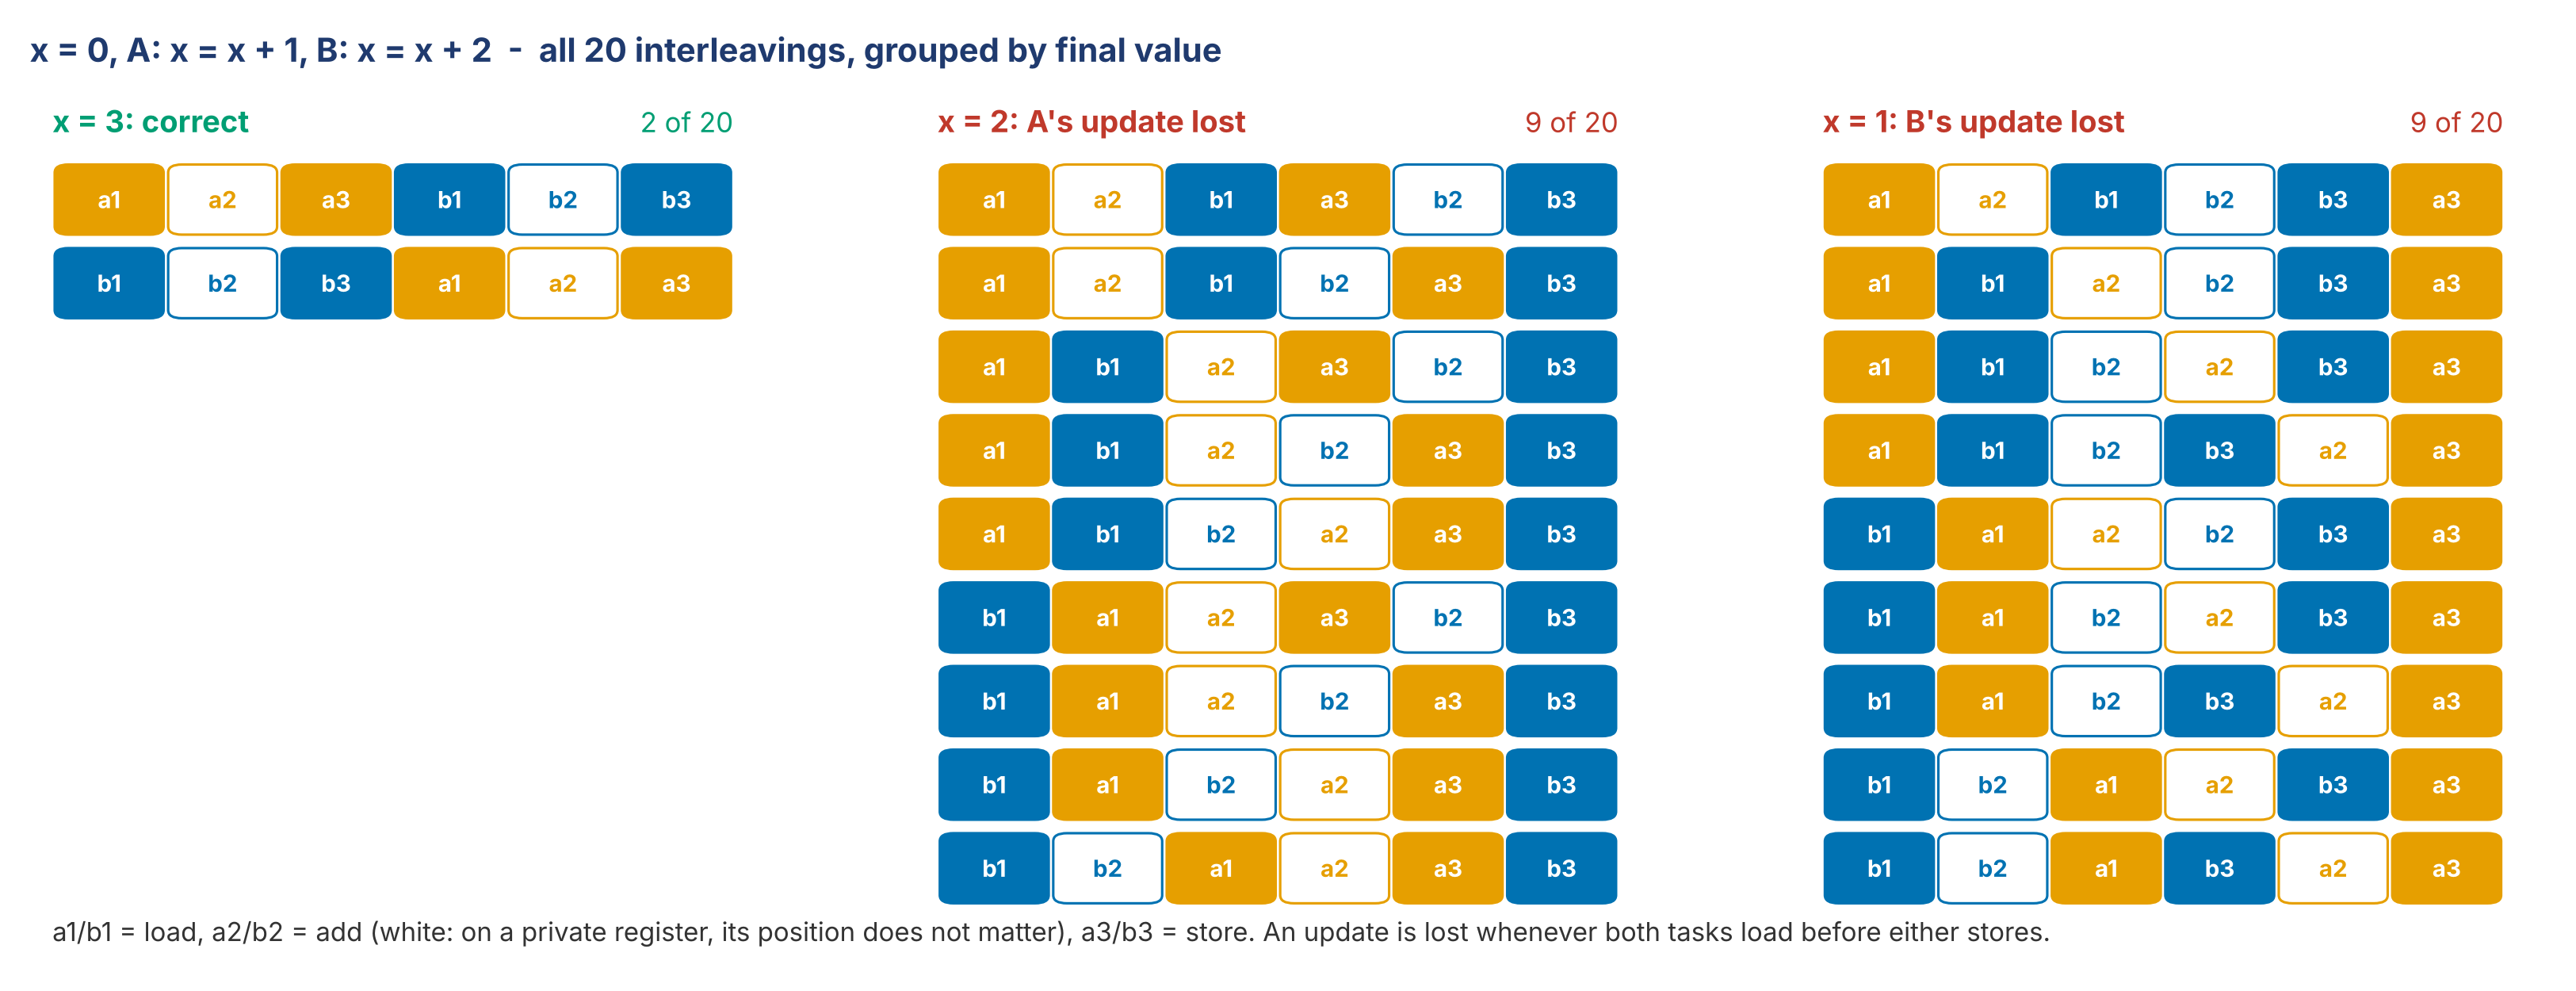
\includegraphics[width=1\textwidth]{contents/images/week-07/interleavings_results.png}
    \caption{\texttt{x = 0}, A fa \texttt{x + 1}, B fa \texttt{x + 2}: tutti i 20 interleaving, raggruppati per risultato. Solo i due ordini sequenziali danno 3; negli altri 18 entrambi caricano 0 prima di scrivere, e vince l'ultimo store. Le celle bianche (le somme) si possono spostare senza cambiare nulla.}
\end{figure}

\paragraph*{Esempi svolti.}
\begin{itemize}
    \item \texttt{x = 0}, A fa \texttt{x + 1}, B fa \texttt{x + 2}: risultati possibili \textbf{1, 2, 3}; solo 3 è corretto (1: vince A con $0+1$; 2: vince B con $0+2$).
    \item \texttt{x = 1}, A fa \texttt{x * 2}, B fa \texttt{x + 3}: A poi B dà $(1 \cdot 2) + 3 = 5$; B poi A dà $(1 + 3) \cdot 2 = 8$; se entrambi caricano 1 prima di scrivere, si ottiene 2 (A scrive per ultimo) o 4 (B per ultimo). Valori possibili \textbf{2, 4, 5, 8}; corretti 5 e 8 (il programma non dice chi va prima). Se load-calcolo-store non si può tagliare, restano solo 5 e 8.
    \item \texttt{x = 0}, A e B fanno \texttt{x = x + 1} \textbf{due volte} ciascuno: massimo \textbf{4} (nessuna sovrapposizione), minimo \textbf{2}. \textbf{1 è impossibile}, e all'esame va \emph{spiegato}, non solo detto: ogni store scrive almeno 1. L'ultimo store della run appartiene al \emph{secondo} incremento di qualche task, il cui load viene dopo il primo store dello stesso task, che ha scritto almeno 1; quindi quel load legge almeno 1 e lo store scrive almeno 2. Una risposta come ``perché B sovrascrive'' all'esame non basta.
\end{itemize}

\subsubsection*{5. Gli strumenti, dal più semplice}
\paragraph*{Mascherare gli interrupt.} Su una CPU sola un task perde la CPU solo per un interrupt (tick, poi PendSV) o per una sua chiamata (yield, delay, exit). Se si mascherano gli interrupt, nessuno entra. Il kernel lo fa già in \texttt{uart\_write}: \texttt{irq\_save()} (\texttt{mrs r0, primask}, poi \texttt{cpsid i}) e \texttt{irq\_restore( saved )}, che rimette il \emph{vecchio} valore e quindi permette sezioni annidate. Ha però quattro limiti:
\begin{itemize}
    \item \textbf{solo codice privilegiato}: in un task unprivileged \texttt{cpsid i} viene \textbf{ignorata}, senza fault e senza effetto. Con \texttt{DEMO=cpsid} le righe si mescolano ancora (12 rotte in una run). È voluto: un task che può mascherare può fermare il tick e tenersi la CPU per sempre;
    \item \textbf{latenza}: finché è mascherato il sistema non risponde a niente, quindi va fatto solo per poche istruzioni;
    \item \textbf{un solo core}: su un multi-core maschera solo il proprio core;
    \item quindi va bene \textbf{dentro il kernel}, o in un sistema ``piatto'' tutto privilegiato.
\end{itemize}

\paragraph*{Un flag semplice non funziona.} \texttt{while ( busy == 1 ) \{\}} e poi \texttt{busy = 1}: il \emph{test} e il \emph{set} sono due istruzioni. A legge 0, switch, B legge 0, scrive 1 ed entra, switch, A scrive 1 ed entra anche lui. È di nuovo un lost update, stavolta sul flag. Serve che test e set siano \textbf{un unico passo atomico}, e da solo il software non ci riesce: serve l'hardware.

\paragraph*{L'aiuto dell'hardware.} Il classico è il \textbf{test-and-set}: in un passo solo legge il vecchio valore e scrive 1 (su x86, ad esempio \texttt{xchg}). Se restituisce 0, il lock era libero e ora è tuo; se restituisce 1, era già preso. Il Cortex-M3 (RISC) non ha un'istruzione simile, e divide il lavoro in due:
\begin{itemize}
    \item \texttt{ldrex r1, [r0]}: un load normale, che però attiva l'\textbf{exclusive monitor} sull'indirizzo (stato \emph{Exclusive});
    \item \texttt{strex r2, r1, [r0]}: scrive \emph{solo se} il monitor è ancora Exclusive. \texttt{r2 = 0} vuol dire scritto, \texttt{r2 = 1} vuol dire fallito e niente scritto. In ogni caso il monitor torna \emph{Open};
    \item \textbf{ogni eccezione} (tick, PendSV, system call, UART), in ingresso o in uscita, rimette il monitor a Open. Su una CPU sola un altro task può girare solo dopo un'eccezione, quindi uno \texttt{strex} interrotto dopo il suo \texttt{ldrex} \textbf{fallisce} e il task riprova;
    \item la coppia \textbf{non} è ``ininterrompibile'': o in mezzo non è successo niente, oppure la scrittura non avviene e lo sai.
\end{itemize}

\paragraph*{La barriera \texttt{dmb}.} Le CPU (e i compilatori) possono riordinare gli accessi in memoria. \texttt{dmb} è un punto di controllo: tutti gli accessi prima di lei finiscono prima di qualunque accesso dopo di lei. Regola: \textbf{\texttt{dmb} dopo aver preso il lock} e \textbf{\texttt{dmb} prima di rilasciarlo}. Sul Cortex-M3 costa quasi niente; su core più complessi è ciò che rende il lock corretto.

\paragraph*{Spinlock.} \texttt{ldrex} + \texttt{strex} + \texttt{dmb}, circa 10 istruzioni: chi trova il lock preso \textbf{gira a vuoto} (busy waiting) e riprova. Funziona in codice unprivileged. Su due core ha senso (chi tiene il lock gira sull'altro core); su \textbf{una CPU} è spreco puro, perché chi tiene il lock non può girare mentre tu giri. Da qui lo \textbf{spin-then-yield}: se il lock è preso, chiama \texttt{task\_yield} e riprova al turno successivo.

\paragraph*{Semaforo.} Un contatore intero più una lista di task BLOCKED, con due operazioni atomiche: \textbf{wait} e \textbf{signal} (P e V per Dijkstra, \textbf{take} e \textbf{give} in FreeRTOS).
\begin{itemize}
    \item \texttt{wait}: se \texttt{count > 0} lo decrementa e si prosegue; altrimenti il task diventa BLOCKED e va nella lista. Niente spin: la CPU passa agli altri.
    \item \texttt{signal}: se qualcuno aspetta, ne sveglia uno (BLOCKED $\to$ READY) e \textbf{il count non cambia}, perché il permesso passa direttamente a lui; altrimenti \texttt{count++}.
    \item Richiede tre cose: memoria condivisa per il contatore, test e aggiornamento atomici, e uno scheduler capace di bloccare e risvegliare i task. Per questo lo scratch-OS non lo implementa.
\end{itemize}
\begin{center}
\small
\begin{tabular}{P{0.12} P{0.2} P{0.3} P{0.3}}
    \hline
    \textbf{valore iniziale} & \textbf{tipo} & \textbf{significato} & \textbf{esempio} \\
    \hline
    $N > 1$ & counting & $N$ risorse identiche libere & 2 canali radio per 4 task \\
    1 & binario (mutua esclusione) & un task alla volta & \texttt{wait} = entry, \texttt{signal} = exit \\
    0 & signalling & ``B aspetta finché A dice via'' & l'handler della UART fa \texttt{signal}, B fa \texttt{wait} \\
    \hline
\end{tabular}
\end{center}
Un \texttt{signal} che arriva prima del \texttt{wait} \textbf{non si perde}: il contatore se lo ricorda. Un handler di interrupt può fare \texttt{signal}, perché \texttt{signal} non blocca mai. Un semaforo di mutua esclusione inizializzato a 0 per errore blocca tutti per sempre: nessuno entra e nessuno fa signal, quindi il \emph{progresso} è violato.

\paragraph*{Mutex.} Il ``fratello maggiore'' dello spinlock: chi aspetta si blocca invece di girare, e il mutex ha un \textbf{proprietario}. Solo il task che l'ha preso può rilasciarlo; un unlock da parte di un altro task è un errore che il kernel rileva.
\begin{center}
\small
\begin{tabular}{P{0.28} P{0.32} P{0.32}}
    \hline
    & \textbf{semaforo binario} & \textbf{mutex} \\
    \hline
    proprietario & no & sì \\
    chi può rilasciarlo & qualunque task, anche un handler & solo chi lo tiene \\
    uso tipico & mutua esclusione o segnalazione & solo mutua esclusione \\
    rilascio dal task sbagliato & permesso: bug nascosto & rilevato come errore \\
    \hline
\end{tabular}
\end{center}
\textbf{Regola pratica}: mutex per \textbf{proteggere dati}, semaforo per \textbf{contare o segnalare}.

\begin{center}
\small
\begin{tabular}{P{0.17} P{0.27} c P{0.3}}
    \hline
    \textbf{primitiva} & \textbf{come aspetta un task} & \textbf{owner} & \textbf{quando usarla} \\
    \hline
    mascherare & nessuno aspetta: niente switch & -- & poche istruzioni nel kernel, una CPU \\
    spinlock & gira (o gira e poi cede) & no & sezioni brevi, meglio con più core \\
    semaforo & BLOCKED fino a un \texttt{signal} & no & contare, mutua esclusione, segnalare \\
    mutex & di solito BLOCKED & sì & mutua esclusione \\
    \hline
\end{tabular}
\end{center}
Tutte danno una entry e una exit section; cambia \textbf{come passa il tempo chi aspetta}. Spinlock, semaforo e mutex poggiano sullo stesso test-and-set atomico; semaforo e mutex in più hanno bisogno dello scheduler.

\subsubsection*{6. Tracce dei semafori (tipo d'esame)}
A ogni operazione scrivi \textbf{count}, \textbf{lista} e \textbf{chi è dentro}, applicando le due regole del punto 5. Esempio: semaforo a 1; A wait, B wait, C wait, A signal, B signal.
\begin{center}
\small
\begin{tabular}{l c l l}
    \hline
    \textbf{passo} & \textbf{count} & \textbf{lista} & \textbf{dentro} \\
    \hline
    A \texttt{wait} & 0 & -- & A \\
    B \texttt{wait} & 0 & B & A \\
    C \texttt{wait} & 0 & B, C & A \\
    A \texttt{signal} & 0 & C & B (READY con il permesso di A) \\
    B \texttt{signal} & 0 & -- & C (READY con il permesso di B) \\
    \hline
\end{tabular}
\end{center}
Il count resta 0 fino alla fine, perché a ogni \texttt{signal} c'è qualcuno in attesa. Torna a salire solo quando un \texttt{signal} non trova nessuno.

\subsubsection*{7. Mai contare sull'ordine}
Chi entra per primo, e chi viene svegliato dopo un \texttt{signal} (B o C?), lo decide lo \textbf{scheduler}, non l'ordine in cui i task hanno chiamato \texttt{wait}. Le tabelle degli esercizi fanno un'ipotesi, ma un'applicazione che funziona solo perché ``dopo questo signal tocca a B'' si rompe il giorno in cui un aggiornamento del sistema operativo cambia lo scheduler. \textbf{L'analogia del bagno}: un solo bagno in un bar, tante persone in coda. Quando la porta si apre, decide il proprietario chi entra; lui promette solo che se il bagno è libero e vuoi entrare puoi andare (\emph{progresso}), e che non aspetterai per sempre (\emph{attesa limitata}). Nient'altro.

\subsection{Unità 2}
\paragraph*{L'obiettivo.} Sistemare le due race dello scratch-OS con uno spinlock vero. Il punto di partenza è il kernel della settimana 5 (round robin, \texttt{task\_yield}, trace), con un programma in due fasi: prima il contatore condiviso, poi 3000 righe di lettere per task. È già tutto pronto attorno al lock: la regione condivisa, l'MPU, le chiamate nei task. Mancano solo le tre funzioni in \texttt{lib/spinlock.s}, che nella base sono un semplice \texttt{bx lr}. Si scrivono in \textbf{assembly}, perché servono \texttt{ldrex} e \texttt{strex}. (Percorsi relativi a \texttt{scratch-os/week-07/solution/}.)

\subsubsection*{1. Memoria condivisa tra task isolati}
Dalla settimana 4 ogni task vede solo la sua partizione. Per condividere un dato serve un blocco di RAM aperto a tutti e due:
\begin{itemize}
    \item nel linker script (\texttt{scripts/mps2\_m3.ld}) c'è una sezione \texttt{.shared}, \texttt{ALIGN(1024)}, \texttt{(NOLOAD)}, lunga sempre esattamente 1\,KB: si trova a \texttt{0x20003000}, subito dopo le tre partizioni da 4\,KB;
    \item \textbf{MPU region 2}, impostata una volta sola in \texttt{mpu\_init} (\texttt{kernel/mpu.c}): \texttt{RBAR} $=$ \texttt{0x20003012} (indirizzo $|$ VALID $|$ 2), \texttt{RASR} $=$ \texttt{0x13060013} (XN, lettura-scrittura per tutti, 1\,KB, abilitata). Uno switch riscrive solo la region 1, quindi la region 2 \textbf{non cambia mai};
    \item una variabile ci finisce con il marcatore \texttt{SHARED} (\texttt{\_\_attribute\_\_(( section( ".shared" ) ))}), ad esempio \texttt{volatile uint32\_t shared\_counter SHARED;} in \texttt{src/shared.c}.
\end{itemize}
Tre domande della slide:
\begin{itemize}
    \item \emph{Perché una variabile condivisa non può avere un valore iniziale?} \texttt{NOLOAD} significa che in FLASH non c'è nessuna copia, quindi nessuno la inizializza: parte da 0, e un \texttt{= 5} si perde in silenzio. Per i lock va benissimo: \textbf{0 = libero}.
    \item \emph{Perché 1\,KB e allineato a 1\,KB?} Regole dell'MPU (settimana 4): una regione ha una dimensione potenza di due ed è allineata alla sua dimensione.
    \item \emph{Perché \texttt{printf( "...\%u", shared\_counter )} funziona, se \texttt{sys\_write} accetta solo buffer nella partizione del task?} \texttt{printf} \textbf{copia}: formatta nel suo buffer sullo stack del task, e il contatore le arriva \textbf{per valore}, in un registro.
\end{itemize}

\subsubsection*{2. \texttt{LOCK} e \texttt{UNLOCK}: un programma, tre comportamenti}
I task chiamano sempre \texttt{LOCK( \&counter\_lock )} e \texttt{UNLOCK( \&counter\_lock )}; il Makefile decide che cosa diventano:
\begin{center}
\small
\begin{tabular}{P{0.4} P{0.27} P{0.23}}
    \hline
    \textbf{build} & \texttt{LOCK} & \texttt{UNLOCK} \\
    \hline
    \texttt{DEMO=race}, \texttt{counter}, \texttt{cpsid} & niente (\texttt{do \{\} while(0)}) & niente \\
    \texttt{DEMO=spin} & \texttt{spin\_lock\_busy} & \texttt{spin\_unlock} \\
    \texttt{make run} (default) & \texttt{spin\_lock} & \texttt{spin\_unlock} \\
    \hline
\end{tabular}
\end{center}
\begin{itemize}
    \item Si passa l'\textbf{indirizzo} del lock, perché la funzione deve modificare la parola nella regione condivisa, non una copia. Per l'AAPCS arriva in \texttt{r0}.
    \item \texttt{spinlock\_t} è un \texttt{volatile uint32\_t}, perché l'altro task lo cambia ``alle spalle'' del compilatore.
    \item Ci sono \textbf{due} lock, uno per risorsa: \texttt{counter\_lock} e \texttt{uart\_lock}. Chi stampa non impedisce all'altro di contare.
\end{itemize}

\subsubsection*{3. \texttt{spin\_lock\_busy} e \texttt{spin\_unlock}}
\begin{lstlisting}[basicstyle=\ttfamily\scriptsize]
spin_lock_busy:
spin_lock_busy_try:
    ldrex r1, [r0]               /* leggi il lock, il monitor diventa Exclusive */
    cmp r1, #0                   /* libero? */
    bne spin_lock_busy_try       /* preso: rileggi (busy waiting) */
    mov r1, #1                   /* 1 = preso */
    strex r2, r1, [r0]           /* prova a scrivere 1: r2 = 0 ok, 1 fallito */
    cmp r2, #0
    bne spin_lock_busy_try       /* fallito: qualcosa si e' messo in mezzo, riprova */
    dmb                          /* da qui iniziano gli accessi protetti */
    bx lr                        /* il lock e' tuo */

spin_unlock:
    dmb                          /* prima finisci gli accessi della sezione critica */
    mov r1, #0
    str r1, [r0]                 /* store normale: il lock e' libero */
    bx lr
\end{lstlisting}
\begin{itemize}
    \item \textbf{Attenzione al significato di \texttt{r2}}: 0 vuol dire scritto con successo, 1 vuol dire fallito. In aula il professore l'ha detto al contrario una volta.
    \item L'unlock è uno \textbf{store normale}: solo chi tiene il lock scrive su quella parola, e l'\texttt{strex} dell'altro scrive solo dopo aver letto 0, cosa impossibile finché il lock vale 1.
    \item Usano solo \texttt{r0}--\texttt{r2}, che una funzione chiamata può modificare: niente \texttt{push}/\texttt{pop}.
    \item Le direttive (\texttt{.global}, \texttt{.type}, \texttt{.thumb\_func}, \texttt{.size}) sono quelle degli stub della settimana 4. \texttt{spin\_lock\_busy\_try} è una seconda etichetta allo stesso indirizzo, che rende chiaro il significato del salto (``riprova'').
    \item Questo codice dipende dalla CPU: va riscritto per ogni porting del sistema operativo.
\end{itemize}

\begin{figure}[H]
    \centering
    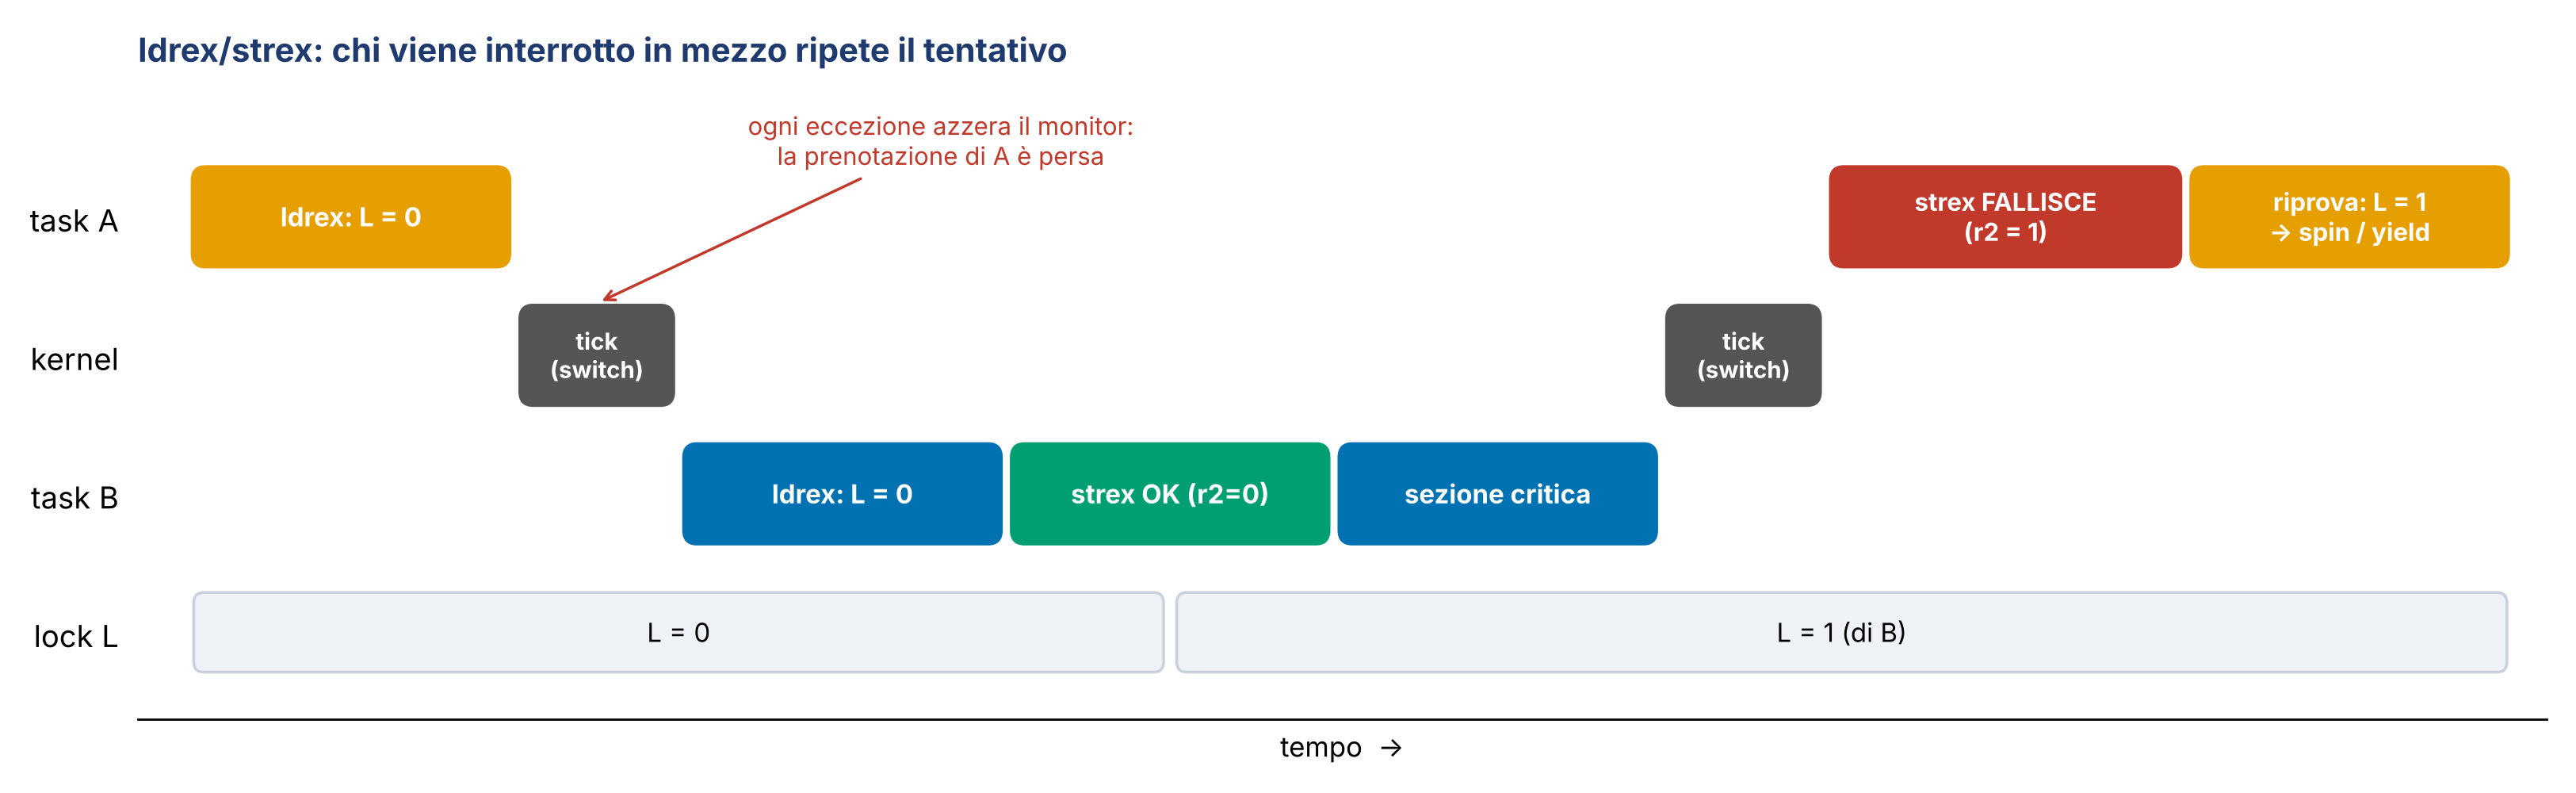
\includegraphics[width=1\textwidth]{contents/images/week-07/it_strex_fail.png}
    \caption{Perché il lock regge alla preemption. A legge il lock libero, ma il tick (un'eccezione) riporta il monitor a Open; B prende il lock; quando A torna, il suo \texttt{strex} fallisce (\texttt{r2 = 1}), A rilegge il lock, lo trova a 1 e aspetta. Per questo \texttt{PendSV\_Handler} non ha bisogno di \texttt{clrex}.}
\end{figure}

\subsubsection*{4. \texttt{DEMO=spin}: corretto, ma caro}
\begin{itemize}
    \item \texttt{counter=2000000} a ogni run, e tutte le 6000 righe sono intere.
    \item Il trace sembra il round robin della settimana 5, slot da 5 tick, ma \textbf{non può mostrare} quali slot hanno fatto lavoro utile: per il kernel un task che gira a vuoto è RUNNING come uno che conta.
    \item Nella fase del contatore chi tiene il lock lo tiene quasi tutto il giro (dentro c'è \texttt{plus\_one}), quindi il tick cade quasi sempre col lock preso, e l'altro task \textbf{spreca l'intero slot}: su una CPU sola, chi tiene il lock non può girare mentre tu giri.
    \item Costo: circa \textbf{259 tick} in media (da 210 a 280, a seconda di dove cade il tick), contro circa 112--115 della base senza lock, che però dà un risultato sbagliato.
\end{itemize}

\subsubsection*{5. Spin-then-yield: \texttt{spin\_lock}}
Se il lock è preso non serve riprovare subito: chi lo tiene è l'\emph{altro} task, che non può girare. Quindi si cede la CPU:
\begin{lstlisting}[basicstyle=\ttfamily\scriptsize]
spin_lock:
spin_lock_try:
    ldrex r1, [r0]
    cmp r1, #0
    bne spin_lock_wait           /* preso: cedi la CPU */
    mov r1, #1
    strex r2, r1, [r0]
    cmp r2, #0
    bne spin_lock_try            /* strex fallito: riprova SUBITO */
    dmb
    bx lr
spin_lock_wait:
    push {r0, lr}                /* salva indirizzo del lock e indirizzo di ritorno */
    bl task_yield                /* svc #6: intanto gira chi tiene il lock */
    pop {r0, lr}
    b spin_lock_try              /* forse ora e' libero */
\end{lstlisting}
\begin{itemize}
    \item \textbf{Perché salvare \texttt{lr}}: \texttt{bl} scrive in \texttt{lr} il proprio indirizzo di ritorno, cancellando quello verso il codice C del task.
    \item \textbf{Perché salvare \texttt{r0}}: una funzione chiamata può cambiare \texttt{r0}--\texttt{r3}, e \texttt{task\_yield} lo fa davvero (il kernel ci scrive il risultato 0). Ma \texttt{r0} contiene l'indirizzo del lock.
    \item \textbf{Perché due registri e non uno}: l'AAPCS vuole lo stack allineato a \textbf{8 byte} a ogni chiamata, quindi si fa \texttt{push} di un numero \textbf{pari} di registri. Anche senza \texttt{r0} da salvare, se ne spingerebbero comunque due.
    \item Il primo \texttt{bne} ora va a \texttt{spin\_lock\_wait}; il secondo, dopo uno \texttt{strex} fallito, torna ancora subito al \texttt{ldrex}.
    \item Un \texttt{ldrex} senza \texttt{strex} lascia il monitor Exclusive, ma è innocuo: la \texttt{svc} di \texttt{task\_yield} è un'eccezione e lo azzera.
\end{itemize}
\begin{figure}[H]
    \centering
    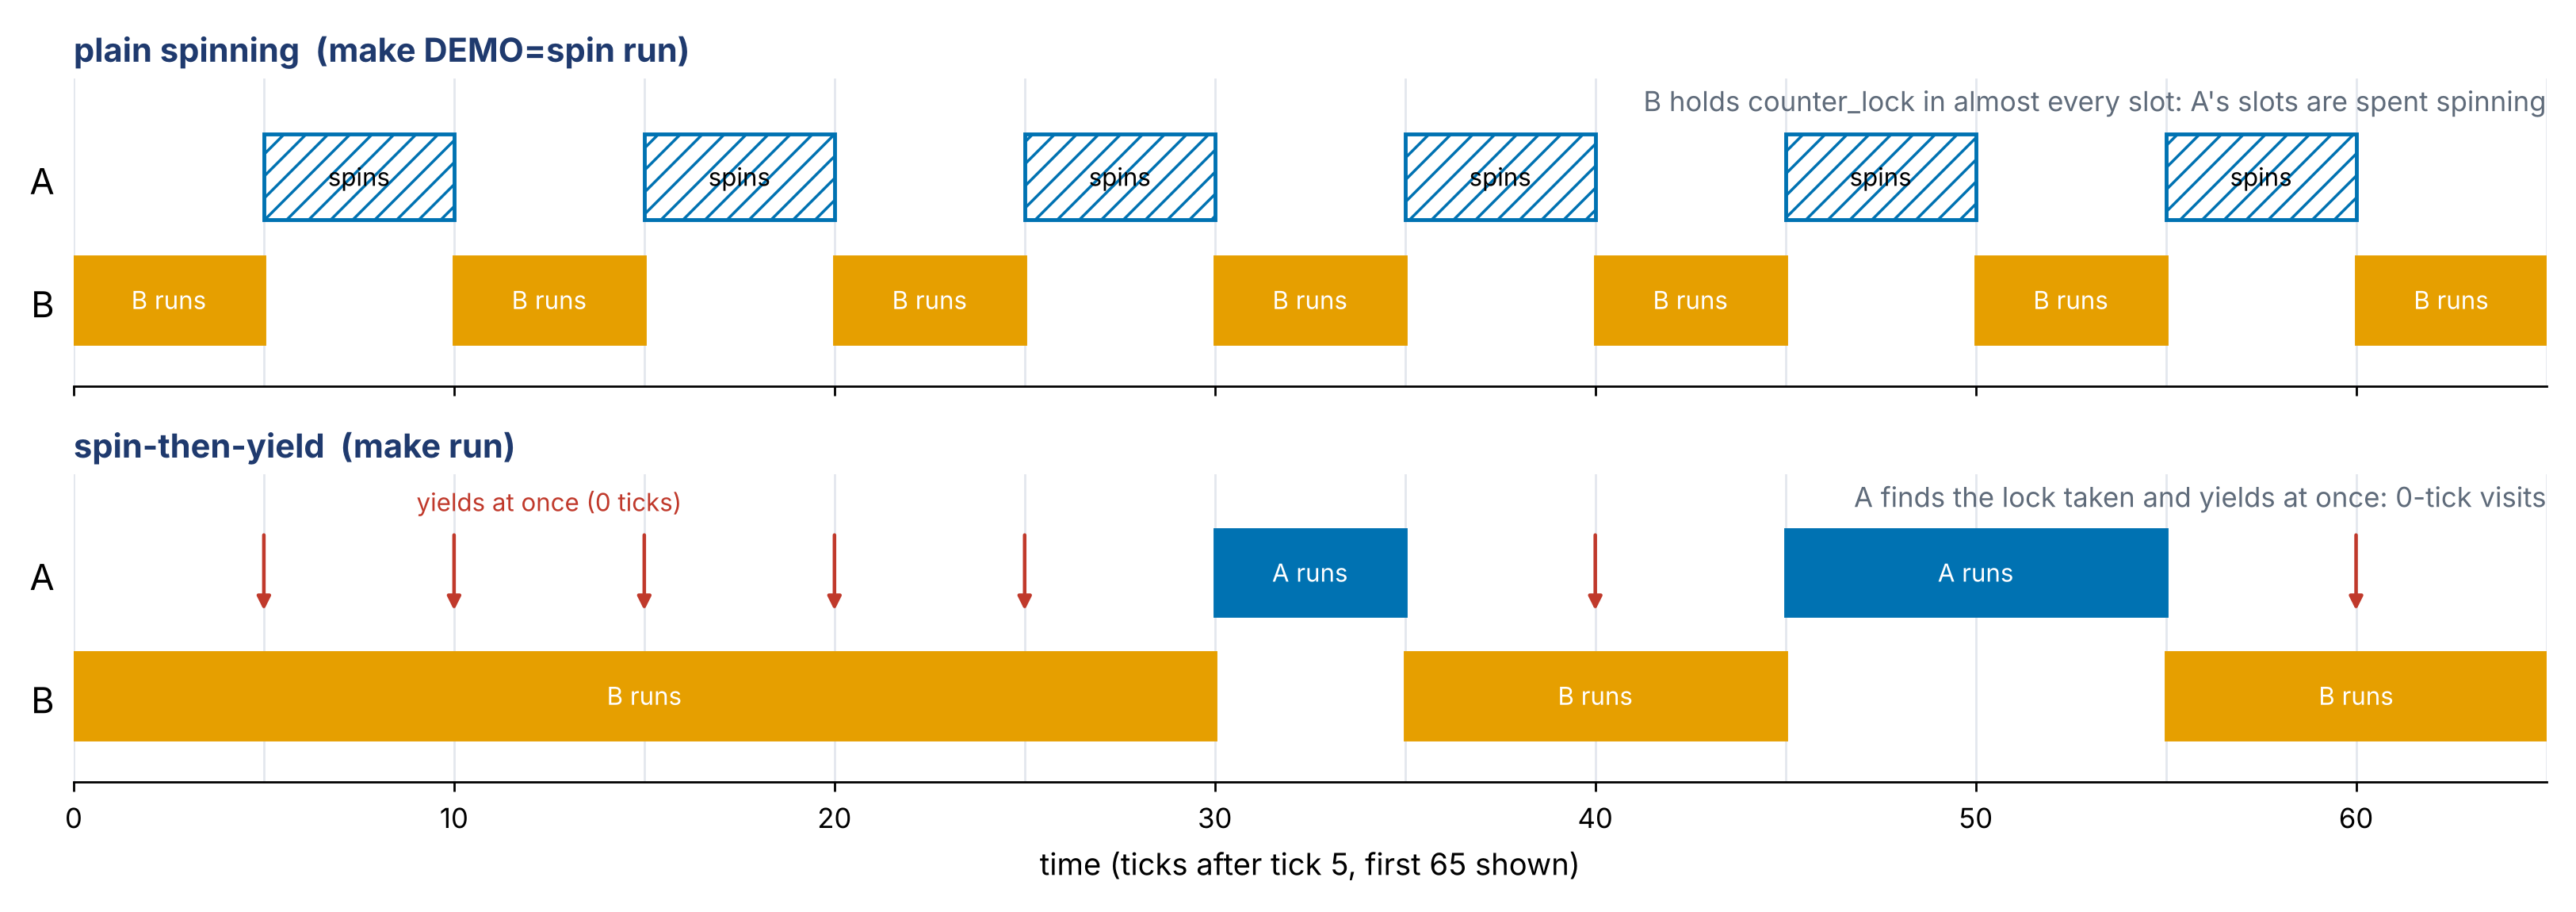
\includegraphics[width=1\textwidth]{contents/images/week-07/spin_vs_yield.png}
    \caption{Gli stessi 65 tick con i due lock. Con lo spin puro gli slot di chi aspetta sono tutti sprecati, ma il trace non lo mostra; con spin-then-yield le visite di chi aspetta durano 0 tick, e chi tiene il lock resta in CPU per molti slot di fila.}
\end{figure}
\begin{center}
\small
\begin{tabular}{P{0.3} P{0.22} P{0.13} P{0.25}}
    \hline
    \textbf{build} & \textbf{lock} & \textbf{risultato} & \textbf{ultimo tick (media)} \\
    \hline
    base, nulla scritto & nessuno & sbagliato & circa 112 \\
    \texttt{make DEMO=spin run} & \texttt{spin\_lock\_busy} & corretto & circa 259 \\
    \texttt{make run} & \texttt{spin\_lock} & corretto & circa 171 \\
    \hline
\end{tabular}
\end{center}
\emph{Perché spin-then-yield è comunque più lento di nessun lock?} Perché le 2\,000\,000 coppie lock/unlock costano (\texttt{ldrex}, \texttt{strex}, \texttt{dmb}), e ogni visita di chi aspetta costa una system call e due switch, anche se dura 0 tick. La base è più veloce solo perché fa meno lavoro, e sbaglia: \textbf{una risposta veloce ma sbagliata non è una risposta}. In più spin-then-yield è \textbf{prevedibile}: circa 171 a ogni run.

\subsubsection*{6. Che cosa garantisce lo spinlock, e che cosa no}
\begin{center}
\small
\begin{tabular}{P{0.45} P{0.45}}
    \hline
    \textbf{garantisce} & \textbf{non garantisce} \\
    \hline
    mutua esclusione: tra due \texttt{strex} c'è almeno un'eccezione, quindi il secondo fallisce & equità e attesa limitata: un task può trovare il lock preso a ogni turno \\
    funziona in codice unprivileged, senza system call per un lock libero & attesa gratuita: busy waiting brucia slot interi, lo yield costa una svc e due switch \\
    regge alla preemption: chi è interrotto tra \texttt{ldrex} e \texttt{strex} riprova & controllo del proprietario: \texttt{spin\_unlock} scrive 0 chiunque lo chiami \\
    progresso: se il lock è libero, qualcuno lo prende & uso negli handler: un handler che gira su un lock del task interrotto aspetta per sempre \\
    \hline
\end{tabular}
\end{center}
Regola: il lock si tiene \textbf{per poco}, e mai con un \texttt{task\_delay} dentro. Lo scratch-OS si ferma qui \textbf{per scelta}: un lock bloccante richiederebbe liste di attesa e nuove system call. È l'ultima implementazione di kernel del semestre: da ora in poi il kernel (FreeRTOS) si legge e si usa, ma non si modifica.

\subsection{Unità 3}
\paragraph*{L'idea.} FreeRTOS è un kernel vero, sulla stessa scheda (MPS2-AN385) e nello stesso QEMU. La sorpresa è che è costruito con gli stessi pezzi dello scratch-OS. Il kernel è in \texttt{freertos-labs/FreeRTOS/Source/}, è condiviso tra tutte le settimane e \textbf{non si modifica mai}: si scrivono solo i task in \texttt{apps/}, con il supporto della scheda in \texttt{bsp/} e le impostazioni in \texttt{FreeRTOSConfig.h}.

\subsubsection*{1. Il progetto}
\begin{itemize}
    \item \textbf{Scegliere il programma}: \texttt{make APP=hello run} (oppure \texttt{periodic}, \texttt{starve}). Non si cambia nessun file per compilare un altro programma.
    \item Il percorso del kernel nel \texttt{Makefile} è \textbf{relativo}, perché il percorso del corso contiene spazi. Una sola copia condivisa del kernel significa la stessa versione per ogni settimana, e nessuna modifica per sbaglio.
    \item \texttt{FreeRTOSConfig.h}: tick da \textbf{10\,ms}, preemption attiva, time slicing attivo, \textbf{5 priorità} (0--4), heap da \textbf{64\,KB}, stack minimo 256 word $=$ \textbf{1\,KB}, \texttt{configASSERT} e controllo dello stack overflow a ogni switch (le funzioni che stampano l'errore e fermano tutto sono in \texttt{bsp/hooks.c}).
    \item Il kernel non si estende modificandolo, ma con gli \textbf{hook}: funzioni esterne che il kernel chiama in punti precisi e che definisci tu (nomi che finiscono in \texttt{Hook}), abilitate in \texttt{FreeRTOSConfig.h}.
\end{itemize}

\subsubsection*{2. Gli stessi meccanismi, con altri nomi}
\begin{center}
\small
\begin{tabular}{P{0.4} P{0.5}}
    \hline
    \textbf{scratch-OS (settimana 5)} & \textbf{FreeRTOS (port \texttt{ARM\_CM3})} \\
    \hline
    \texttt{struct tcb}, \texttt{sp} come primo campo & \texttt{TCB\_t}, \texttt{pxTopOfStack} come primo campo \\
    campo \texttt{state} & \textbf{la lista} in cui si trova il task (ready, delayed, suspended) \\
    campo \texttt{wake\_tick} & il valore dell'elemento nella lista \emph{delayed}, ordinata \\
    array \texttt{tasks[]} & TCB e stack presi dall'\textbf{heap} (\texttt{xTaskCreate}) \\
    \texttt{task\_init\_stack} (frame finto) & \texttt{pxPortInitialiseStack} (\texttt{port.c}) \\
    PendSV in \texttt{pendsv.s} & \texttt{xPortPendSVHandler} \\
    SysTick $\to$ \texttt{task\_increment\_tick} & \texttt{xPortSysTickHandler} $\to$ \texttt{xTaskIncrementTick} \\
    \texttt{svc \#5}, \texttt{task\_start\_first} & \texttt{vPortSVCHandler} / \texttt{prvPortStartFirstTask} \\
    \texttt{task\_switch\_context} & \texttt{vTaskSwitchContext} \\
    \texttt{idle\_task} (con \texttt{wfi}) & \texttt{prvIdleTask} (gira a vuoto, libera i task cancellati) \\
    \hline
\end{tabular}
\end{center}
Dettagli da sapere:
\begin{itemize}
    \item \textbf{Frame finto}: come il nostro, più \texttt{r0 = pvParameters} (il primo argomento, per l'AAPCS) e \texttt{lr = prvTaskExitError}, che ferma tutto con un'asserzione se la funzione del task ritorna. Il nuovo stack viene riempito con \texttt{0xa5a5a5a5}, per controllare quanto ne è stato usato.
    \item \textbf{Context switch}: le stesse 13 istruzioni, con due aggiunte. Salva \texttt{lr} (EXC\_RETURN) e \texttt{r3} sullo stack MSP, e alza BASEPRI attorno alla chiamata in C.
    \item \textbf{Ogni tick}: se nessun delay scade, un solo confronto con \texttt{xNextTaskUnblockTime} e nessun task da scorrere. Il time slice è di 1 tick.
    \item \textbf{Primo task}: invece di saltare gli 8 zeri li estrae; MSP viene azzerato, perché non si torna mai in \texttt{main()}; nPRIV \textbf{non} viene impostato da nessuna parte: in questo port \textbf{tutti i task sono privilegiati} e non c'è MPU.
\end{itemize}

\subsubsection*{3. Nuova idea 1: una lista READY per priorità}
\texttt{pxReadyTasksLists[]} ha una lista per ogni priorità. \texttt{vTaskSwitchContext} parte dalla priorità più alta (\texttt{uxTopReadyPriority}), trova la prima lista non vuota e, al suo interno, fa round robin. Il task in esecuzione \textbf{resta} nella sua lista READY. Il task idle ha priorità 0 ed è sempre READY, quindi la ricerca non scende mai sotto lo 0.
\begin{itemize}
    \item \emph{A e B (priorità 1) e H (priorità 2) sono READY: chi gira?} H. Se H si blocca, A e B a turno, un tick ciascuno.
    \item Si chiama \textbf{preemptive fixed-priority}: le priorità le scegli tu e il kernel non le cambia mai. Gira sempre un task READY della priorità più alta; se ne diventa READY uno più urgente, prende la CPU \textbf{subito}. Non c'è \emph{aging}: un task che non si blocca mai affama tutti quelli sotto (\textbf{starvation}).
\end{itemize}
\begin{figure}[H]
    \centering
    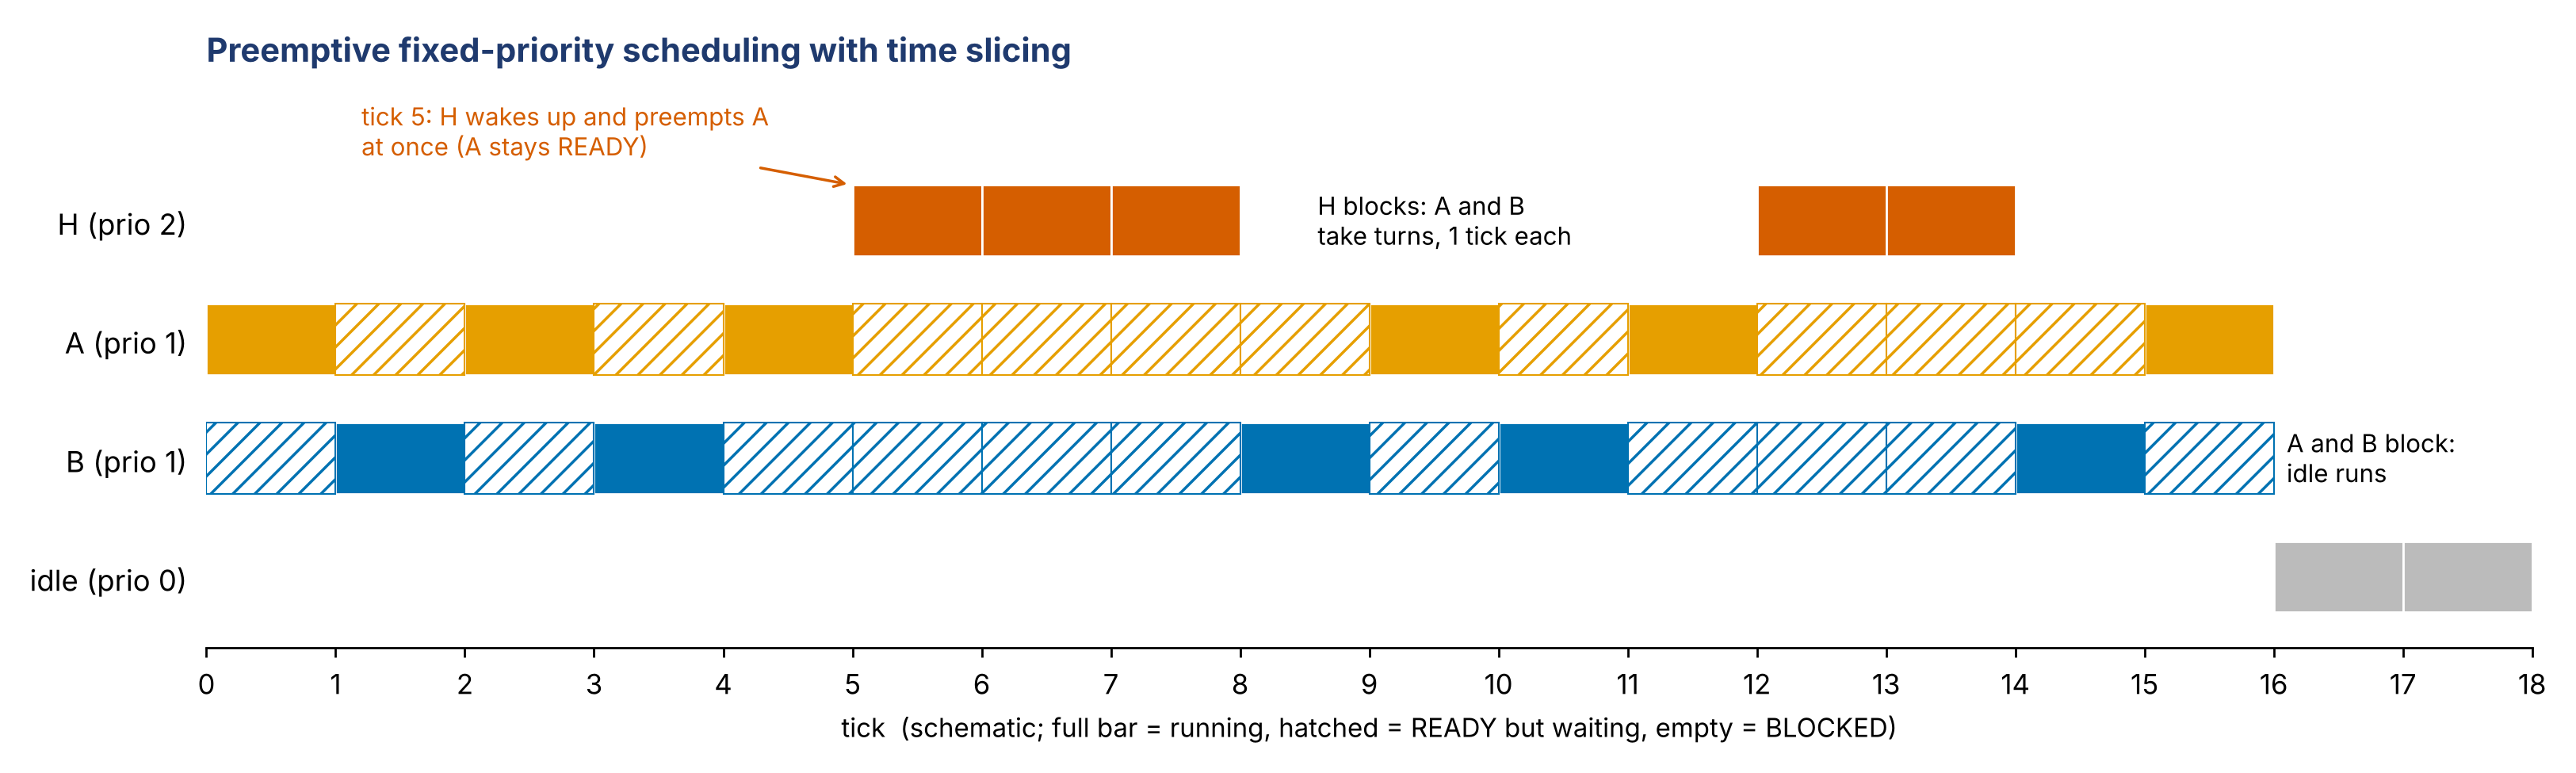
\includegraphics[width=1\textwidth]{contents/images/week-07/preemption.png}
    \caption{Le regole in azione (schema). A e B, stessa priorità, si alternano a ogni tick; H, appena diventa READY, prende subito la CPU e il task interrotto resta READY; quando H si blocca, A e B riprendono a turno; l'idle gira solo quando tutti gli altri sono bloccati.}
\end{figure}

\subsubsection*{4. Nuova idea 2: sezioni critiche con BASEPRI}
\texttt{taskENTER\_CRITICAL()} / \texttt{taskEXIT\_CRITICAL()} (attraverso \texttt{portENTER\_CRITICAL} in \texttt{portmacro.h}) non usano \texttt{cpsid i}: scrivono in \textbf{BASEPRI} il valore 191 (\texttt{configMAX\_SYSCALL\_INTERRUPT\_PRIORITY}, memorizzato come \texttt{0xA0}).
\begin{itemize}
    \item Sono mascherati solo gli interrupt \textbf{meno urgenti} di quella soglia, tra cui SysTick e PendSV (\texttt{0xE0}): dentro una sezione critica non può avvenire \textbf{nessuno switch}. Gli interrupt più urgenti continuano a essere serviti.
    \item Al posto del vecchio valore restituito da \texttt{irq\_save} c'è il contatore \texttt{uxCriticalNesting}: le sezioni si possono annidare, e solo l'ultima uscita smaschera.
    \item Funziona dentro un task (al contrario di \texttt{cpsid} nell'Unità 1) perché i task FreeRTOS sono \textbf{privilegiati}.
\end{itemize}
\paragraph*{\texttt{console\_print}.} È la \texttt{printf} per i task, nel BSP. È lo stesso problema dell'Unità 2, risolto in un altro modo: prima \textbf{formatta l'intera riga} con \texttt{vsnprintf} in un buffer sullo stack del task, \emph{fuori} dalla sezione critica (è lenta, e non tocca niente di condiviso); poi la \textbf{spedisce} tra \texttt{taskENTER\_CRITICAL} e \texttt{taskEXIT\_CRITICAL}. Si usa la macro del kernel e non \texttt{cpsid i} perché tiene il conto dell'annidamento giusto e rispetta le regole del kernel.

\subsubsection*{5. Scrivere un'applicazione FreeRTOS}
\begin{lstlisting}[language=C, showstringspaces=false, basicstyle=\ttfamily\scriptsize]
void vTask( void * pvParameters )             /* prototipo OBBLIGATORIO */
{
    ( void ) pvParameters;                    /* "non lo uso, lo so": niente warning */
    /* set-up, una volta sola */
    for( ;; )                                 /* non deve mai ritornare */
    {
        /* lavoro, poi BLOCCARSI, ad es. vTaskDelay(...) */
    }
}

int main( void )
{
    xTaskCreate( vTask, "A", configMINIMAL_STACK_SIZE, "A", 1, NULL );
    /*           funzione nome  stack in WORD         arg  prio handle */
    vTaskStartScheduler();                    /* crea idle, parte, NON ritorna */
    for( ;; );                                /* solo se l'heap non bastava */
}
\end{lstlisting}
\begin{itemize}
    \item Lo stack si misura in \textbf{word} da 4 byte, non in byte. La priorità va da 0 a 4, dove più alto vuol dire più urgente. Con l'handle \texttt{NULL} non serve un riferimento al task.
    \item \texttt{xTaskCreate} prende TCB e stack dall'heap, costruisce il frame finto e mette il task nella sua lista READY. Si può chiamare \textbf{in qualunque momento}, anche da un altro task.
    \item Un task che ha finito si \textbf{parcheggia} con \texttt{vTaskSuspend( NULL )} (\texttt{NULL} vuol dire ``me stesso''): esce dalle liste READY e non viene più schedulato.
    \item \texttt{pvParameters} è un \texttt{void *}: si può passare una stringa, una struct, un numero (con un cast). Così una funzione serve più task, ognuno con i suoi dati.
    \item \textbf{Convenzioni sui nomi}: \texttt{v} void, \texttt{x} \texttt{BaseType\_t}/struct, \texttt{ux} unsigned, \texttt{px} puntatore, \texttt{pc} \texttt{char *}, \texttt{prv} privata (\texttt{static}).
\end{itemize}

\subsubsection*{6. \texttt{hello}: una funzione, due task}
Un'unica funzione stampa il nome (da \texttt{pvParameters}) e \texttt{xTaskGetTickCount()}, poi \texttt{vTaskDelay( pdMS\_TO\_TICKS( 500 ) )}, cioè 50 tick. L'output è \texttt{B: tick 0}, \texttt{A: tick 0}, \texttt{B: tick 50}, \texttt{A: tick 50}, \dots
\begin{itemize}
    \item \emph{Perché B stampa per primo, se A è creato prima?} Prima che lo scheduler parta, \texttt{xTaskCreate} rende corrente il nuovo task se la sua priorità è \emph{uguale o maggiore}: parte quindi l'\textbf{ultimo creato} tra quelli di priorità massima. L'idle, a priorità 0, non lo sostituisce.
    \item Tra una stampa e l'altra entrambi sono bloccati, e gira l'idle.
\end{itemize}

\subsubsection*{7. \texttt{periodic}: \texttt{vTaskDelay} contro \texttt{vTaskDelayUntil}}
\begin{itemize}
    \item \textbf{\texttt{vTaskDelay( T )}} è \textbf{relativo}: dorme $T$ tick \emph{da quando viene chiamato}, cioè dopo il lavoro. Il prossimo risveglio è a (risveglio + lavoro + $T$), quindi il task \textbf{deriva}. È come \texttt{task\_delay} della settimana 5.
    \item \textbf{\texttt{vTaskDelayUntil( \&last, T )}} è \textbf{assoluto}: dorme fino a \texttt{last + T}, poi \texttt{last += T}. Il lavoro sta \emph{dentro} il periodo e non c'è deriva. È come \texttt{task\_delay\_until}. (È una macro di \texttt{task.h} che chiama \texttt{xTaskDelayUntil}.)
\end{itemize}
\paragraph*{Il template del task periodico} (da sapere a memoria):
\begin{lstlisting}[language=C, showstringspaces=false, basicstyle=\ttfamily\scriptsize]
TickType_t last = xTaskGetTickCount();      /* UNA volta, prima del ciclo */
for( ;; ) { lavoro(); vTaskDelayUntil( &last, T ); }
\end{lstlisting}

\begin{figure}[H]
    \centering
    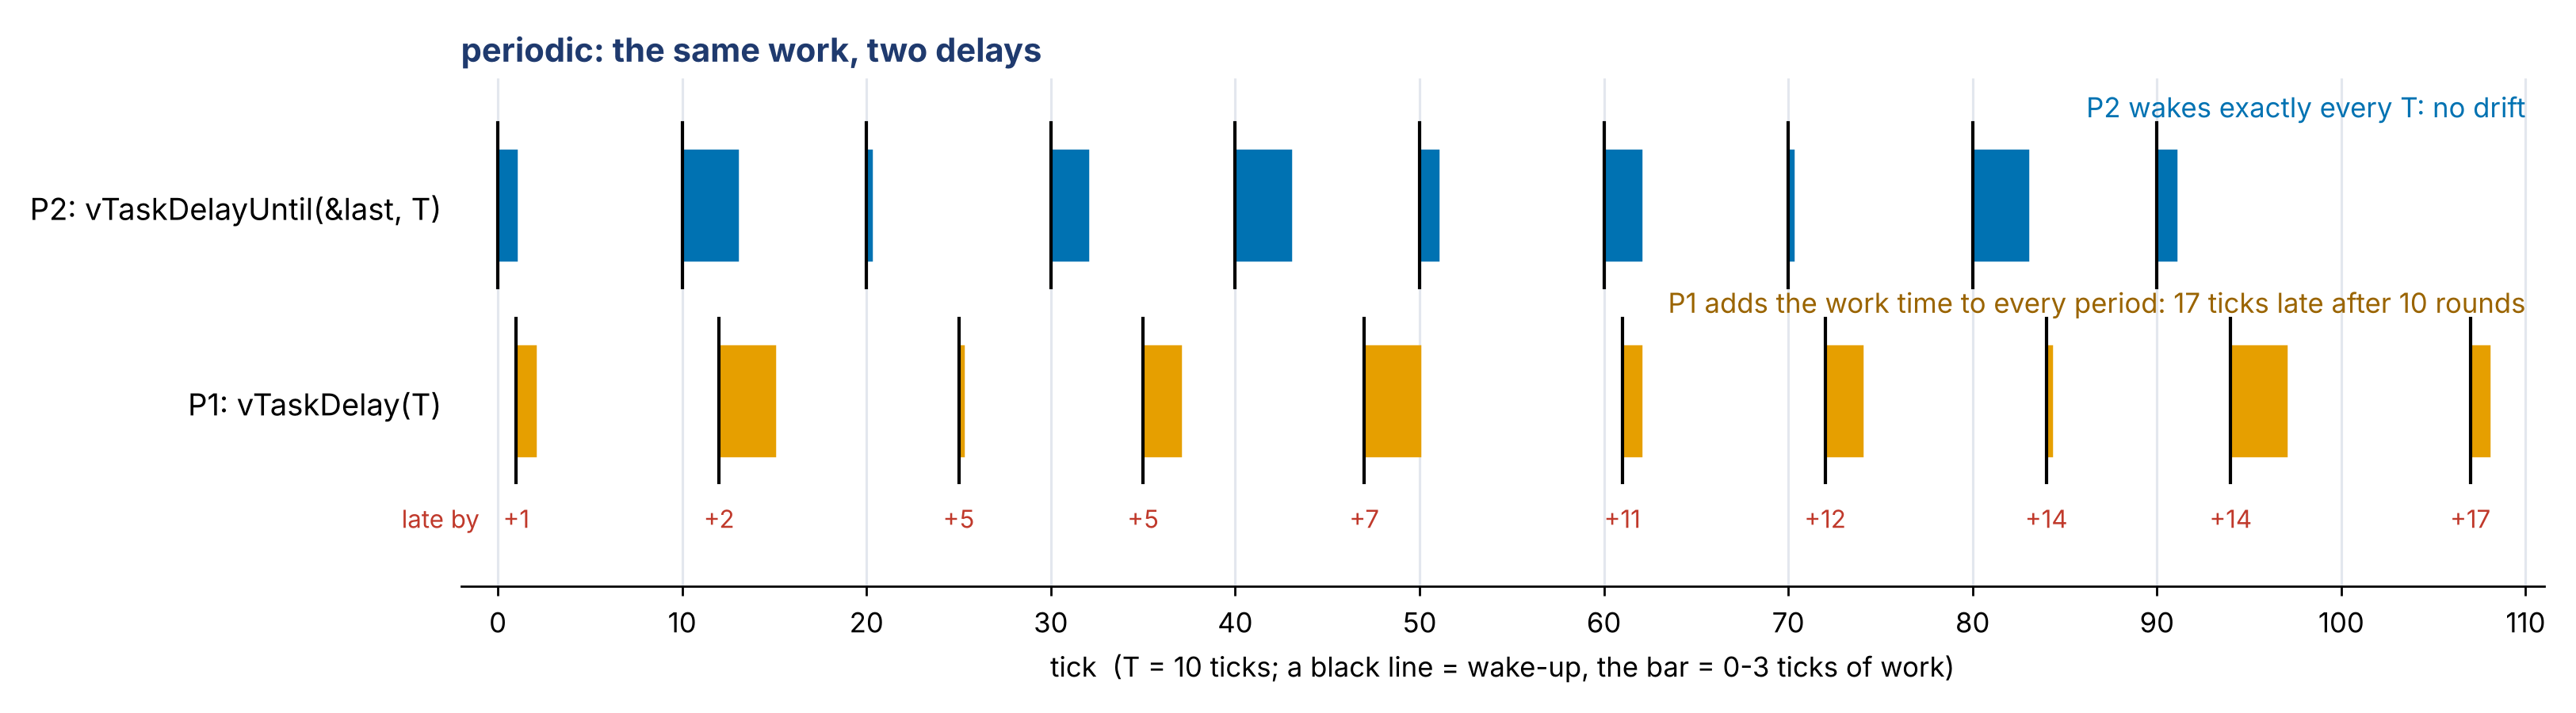
\includegraphics[width=1\textwidth]{contents/images/week-07/periodic_drift.png}
    \caption{La run di \texttt{periodic} con $T = 10$. P2 (\texttt{vTaskDelayUntil}) si sveglia a 0, 10, 20, \dots; P1 (\texttt{vTaskDelay}) a 1, 12, 25, 35, 47, 61, \dots, e dopo 10 giri è in ritardo di 17 tick.}
\end{figure}
Le tre domande della slide:
\begin{itemize}
    \item \emph{Perché P1 deriva?} Nel giro 1 si sveglia a 12, lavora 3 tick fino a 15 e dorme 10, quindi si sveglia a 25. Il lavoro si somma a ogni periodo.
    \item \emph{Perché P1 \#0 è al tick 1 e non 0?} Entrambi sono READY al tick 0 con la stessa priorità: parte P2 (creato per ultimo), che lavora 1 tick, e al tick 1 il time slice passa la CPU a P1.
    \item \emph{Perché 14 tick tra 47 e 61, se $T$ + lavoro fa 13?} P1 lavora da 47 a 50, ma al tick 50 si sveglia P2 che, per il time slicing, prende la CPU per il suo tick di lavoro. P1 chiama \texttt{vTaskDelay} solo al tick 51 e si risveglia a 61. Anche l'attesa della CPU si somma alla deriva.
\end{itemize}

\subsubsection*{8. \texttt{starve}: la starvation e la sua cura}
High (priorità 2) fa lavoro a vuoto (un ciclo \texttt{volatile}, così il compilatore non lo elimina) e stampa, senza mai bloccarsi; Low (priorità 1) stampa e dorme 100\,ms. Con \texttt{DEMO=fixed}, High chiama \texttt{vTaskDelay( 1 )} dopo ogni giro.

\begin{figure}[H]
    \centering
    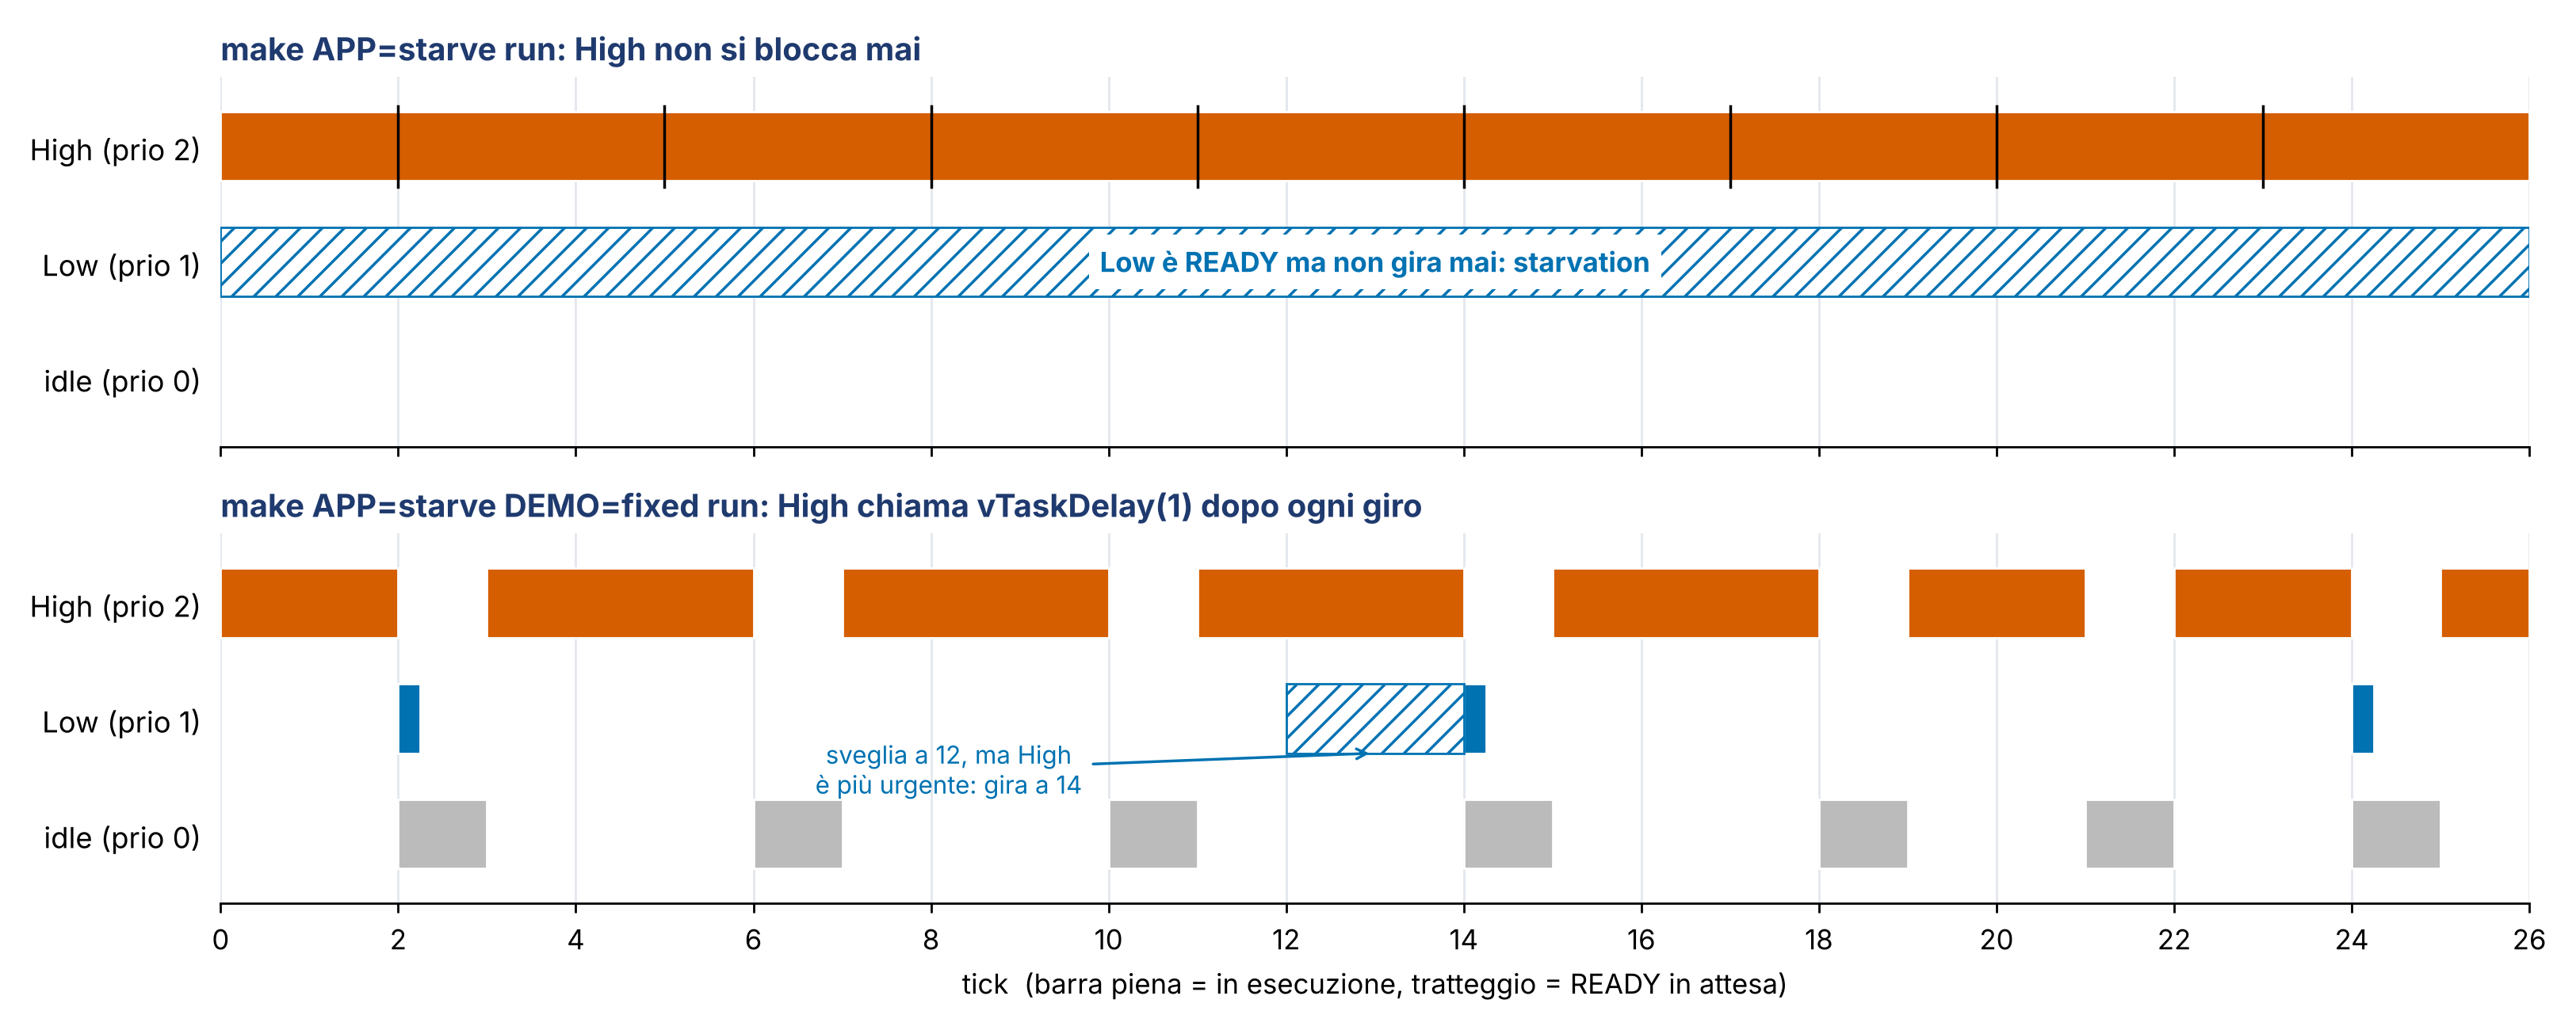
\includegraphics[width=1\textwidth]{contents/images/week-07/it_starve.png}
    \caption{Sopra: High è sempre READY e più urgente, quindi Low non gira mai (starvation). Sotto: con \texttt{vTaskDelay( 1 )} High esce dalla lista READY per un tick dopo ogni giro. Low gira ai tick 2, 14 e 24, e nei buchi restanti gira l'idle.}
\end{figure}
\begin{itemize}
    \item \emph{Perché basta un solo tick?} Quando High si blocca, il task READY più urgente è Low, che gira \textbf{subito}: stampa una riga (pochi microsecondi) e si blocca per 10 tick.
    \item \emph{Perché Low non gira dopo ogni giro di High?} Perché dopo aver stampato è nella lista delayed per 100\,ms; negli altri buchi è READY solo l'idle.
    \item \emph{Perché Low stampa a 14 e non a 12?} Il suo delay finisce a 12, mentre High è a metà di un giro. Low diventa READY ma High è più urgente, quindi Low aspetta il prossimo \texttt{vTaskDelay} di High, al tick 14. Un task meno urgente riceve solo il tempo che i più urgenti lasciano libero.
\end{itemize}
\textbf{La lezione}: un task ad alta priorità deve \textbf{bloccarsi} quando non ha niente di urgente da fare. Anche un delay brevissimo regala la CPU ai task sotto di lui.

\subsubsection*{9. Esame}
Per chi non fa il progetto, la \textbf{seconda parte} dell'esame consiste soprattutto nello scrivere un'\textbf{applicazione FreeRTOS completa}. Anche la prima parte può contenere piccoli esercizi su FreeRTOS (creare un task, cose semplici), oltre agli esercizi su interleaving, lost update e tracce dei semafori dell'Unità 1. Da sapere bene:
\begin{center}
\small
\begin{tabular}{P{0.38} P{0.52}}
    \hline
    \textbf{API / concetto} & \textbf{in una riga} \\
    \hline
    \texttt{void vTask( void *pvParameters )} & set-up, poi \texttt{for( ;; )}; non ritorna mai \\
    \texttt{xTaskCreate( f, nome, stack, arg, prio, handle )} & stack in word; TCB e stack dall'heap \\
    \texttt{vTaskStartScheduler()} & crea l'idle, avvia il primo task, non ritorna \\
    \texttt{vTaskSuspend( NULL )} & parcheggia il task corrente \\
    \texttt{vTaskDelay( T )} & relativo: deriva del tempo di lavoro \\
    \texttt{vTaskDelayUntil( \&last, T )} & assoluto: periodo esatto, niente deriva \\
    \texttt{xTaskGetTickCount()}, \texttt{pdMS\_TO\_TICKS( ms )} & tick correnti; millisecondi $\to$ tick (500\,ms $=$ 50) \\
    \texttt{console\_print( fmt, ... )} & formatta tutta la riga, poi la spedisce in sezione critica \\
    priorità & la più alta READY gira, le pari a turno ogni tick, chi non si blocca affama chi sta sotto \\
    \hline
\end{tabular}
\end{center}
